% Hypothesis
% \begin{itemize}
%     \item Separability is important
%     \begin{itemize}
%         \item Separation sets
%         \item All positive network
%     \end{itemize}
%     \item Controlling separability enhances the network
%     \begin{itemize}
%         \item Depth
%         \item Dead units
%         \item Zero init
%         \item Moons data shattering
%     \end{itemize}
%     \item Separability works in real world
%     \begin{itemize}
%         \item Toy Cifar
%         \item SimpNet
%         \item ULMfit
%         \item Fixup
%     \end{itemize}
% \end{itemize}

\section{Experiments and Results}\label{sec:experiments}
After presenting the separability constraints, we test our formulation in an example of a network according to our formulation (recall the introductory paragraph of section \ref{sec:separability}). Our network has a fixed depth $D=50$ and a fixed layer width of 4 units (i.e. $m_k=4$ for $k=1,\ldots,D$. To which we refuse to perform any architectural modifications. 
\\\\
Our intention is to benchmark our proposal to the most commonly used data manipulation technique: \emph{Batch Normalization} (BN for short). As a consequence, our results entail always a comparison between: (a) no data manipulation, (b) data manipulation via BN and (c) our technique. The only addition introduced during the training is \emph{Adam} \cite{adam}, when calculating gradients \cite{Goodfellow-et-al-2016}.  
\\\\
As a \emph{main} loss we chose to do a comparison between binary cross-entropy (a classic) in \cite{LeCun06atutorial}, and compare it to the case of \emph{no loss} ($\mathcal{L}\equiv 0$ in the introduction of section \ref{sec:separability}). We chose the no loss to explore the nature of the introduction of the separation constraints \emph{by themselves}.     
\\\\
As an initialization for all our experiments we chose two schemes: the Glorot scheme \cite{Glorot10Initialization} (by default on \texttt{Keras}) and a \emph{zero} initialization scheme (setting all parameters to zero), to verify our geometric intuition regarding the distribution of the upper and lower sets of units.   
\\\\
As a dataset, we choose a small version of the \moons dataset, sampling $100$ points ($85$ for training and $15$). Our experiments were done using \texttt{Keras}\cite{keras} and \texttt{TensorFlow}\cite{tensorflow}. We chose the hyperparameters $D$ and $m_k$ to showcase the functioning of our constraints formulation in a particularly \emph{deep} network (as a ratio of depth and layer-width). 
\\\\
We chose the \moons for its \emph{simplicity} in terms of point distribution (two classes parametrically created, see for example Figure \ref{fig:zerosInput3000} on top). Also, the separating functions $F$ created can be easily visualized in a surface map as showcased in Figure \ref{fig:zerosInput3000} (recall equation \ref{eq:network}). In this sense, it is easy to tell whether a classification is \emph{well done} (graphically) and we can relate it to accuracy values. The \moons dataset promotes intuition beyond scores or metrics.  

% Beginning of the experimental section.
\subsection{Effect of the separation on the internal representations}\label{subsec:internalRepresentation}

In terms of accuracy \ReLU reaches a trivial accuracy of $0.51$ while \ReLUBN reaches $0.60$, both architectures fail to solve the problem. When comparing the results presented in Figures \ref{fig:moonsReLU} and \ref{fig:moonsReLUBN}, we find that at the fourth layer \ReLU has collapsed the points of the dataset over a line (parts \ref{fig:moonsReLU41} and \ref{fig:moonsReLU42}), while \ReLUBN still manages to warp the dataset. However, both methods at layer 25th have \emph{collapsed} the dataset into a small number of points (see Figures \ref{fig:moonsReLUBN251}, \ref{fig:moonsReLUBN252} for \ReLUBN and Figures \ref{fig:moonsReLU251} and \ref{fig:moonsReLU252} for \ReLU) that is then \emph{pushed} to the point zero for \ReLU (as shown in the feature layer: \ref{fig:moonsReLUFeature1} and \ref{fig:moonsReLUFeature2}), while \ReLUBN collapses to few points (Figures \ref{fig:moonsReLUBNFeature1} and \ref{fig:moonsReLUBNFeature2}). 
\\\\
We suggest that this collapsing is due the fact that entire portions of the data set are being mapped to the intersection of the lower sets of all the units in a layer, incrementally. Moreover, the likelihood of this collapsing (and its effect on the whole dataset) increases with depth and decreases with width (i.e. bruteforcing non trivial activations via \emph{width-increase}). 
\\\\
In addition, since the gradient is only back-propagated through the points lying on the upper sets of units, geometric collapse also stops learning. Notice that the standarization and the affine transformation (dependent on $\gamma$ and $\beta$) from \ReLUBN are not able to prevent sending the dataset to the lowers of the units. Thus, training thin and deep neural networks is difficult with \ReLU or \ReLUBN.
\\\\
On the extent of our experimentation  \ReLU networks featuring separation constraints are able to solve the problem with higher degrees of accuracy than \ReLU and \ReLUBN (see the figures in Table \ref{tab:moons}). Moreover, Figures \ref{fig:moonsUnitwiseOutput}, \ref{fig:moonsLayerwiseOutput}) \ref{fig:moonsUnitwiseOutput} and \ref{fig:moonsPointwiseOutput}), show that the separation function behaves \emph{intuitively} in the sense of Hauser \& Asok \cite{hauserAsok}. 
\\\\ 
The internal representations not only are non-trivial (as in \ReLUBN) but also preserve geometrical structures like shape and connectivity, as shown in Figures \ref{fig:moonsLayerwise251}, \ref{fig:moonsUnitwise251}, \ref{fig:moonsPointwise251} or \ref{fig:moonsUnitpointwise252}. Indeed, Figures \ref{fig:moonsUnitwise42}, \ref{fig:moonsUnitpointwise42}, \ref{fig:moonsLayerwise42} and \ref{fig:moonsPointwise42} showcase how at the 4th layers a much a solution is already found. This proves that the gradient of the main loss is back-propagated to the input, unlike \ReLU and \ReLUBN (Figures \ref{fig:moonsReLU41}, \ref{fig:moonsReLU41}, \ref{fig:moonsReLUBN41}, \ref{fig:moonsReLUBN42}).
\\\\
The constraints enforce richer representations when used without main loss (cross-entropy), see Figure \ref{fig:init}. In the case of \SepLayer the dataset is mapped into a line (Figures \ref{fig:layerwiseInit501} and \ref{fig:layerwiseInit502}) , whereas the representation reached by \SepUnitPoint is more complex, yet preserves connectivity. Furthermore, both avoid mapping the entire dataset to few values as observed with \ReLU (Figures \ref{fig:reluBNInit501} and \ref{fig:reluBNInit502}) and \ReLUBN (Figures \ref{fig:reluInit501} and \ref{fig:reluInit502}). 
\\\\
% Differences among constraints
The only exception is \SepUnit that apparently solves the problem at layer 25th on Figures \ref{fig:moonsUnitwise251} and \ref{fig:moonsUnitwise252}, yet collapses the dataset in two points at the feature layer (Figures \ref{fig:moonsUnitwiseFeature1} and \ref{fig:moonsUnitwiseFeature1}). Our intuition is  is that, although \SepUnit prevents dead/affine units, it cannot prevent points from falling into the intersection lower set of the units of a layer, construeing a \emph{dead point}). The gradient at dead points will be zero, and can only be recovered by another non-dead point moving a unit so that the dead point, \emph{revives}, when being brought back into the upper set of any unit. The \SepPoint separation constraint was designed precisely to prevent the presence of dead points. However, \SepPoint allows affine and dead units (as shown in Figures \ref{fig:moonsPointwise251} and \ref{fig:moonsPointwise252}), so the the decision function reached becomes \emph{simple} (see Figure \ref{fig:moonsPointwiseOutput}). 
\\\\
Therefore, if we combine both \SepUnit and \SepPoint we should have best of both worlds. Figure \ref{fig:moonsUnitPointwise}, shows how \SepUnitPoint is able to separate both classes perfectly (recall the $0.93$ in accuracy from Table \ref{tab:moons}). Furthermore \SepUnitPoint, produces a feature layer that does not concentrate the dataset in two points like \SepUnit, or concentrates the dataset linearly like \SepPoint. In this sense, we argue that  \SepLayer separates classes in the \texttt{MOONS} quite well, although it is a relaxation of \SepUnitPoint. We think this is due to the fact it allows affine units, that are particularly good at forwarding internal representations, as we will detail in the next subsection.

\subsection{The Role of affine, dead and repeated units}\label{sec:roleofdead}

Despite the fact that we intended to avoid dead and affine neurons with our geometrical formulation (recall the predicate $R_1(u) \wedge R_2(u)$ defined on Equation \ref{eq:separabilityDefinition}) the different constraints differ in practice. While $R_1(u) \wedge R_2(u)$ is valid within \SepUnit and extends to layers, \SepLayer and \SepPoint  allow at least one unit to be affine (recall Equation \ref{eq:affineUnit}) while allowing at least another to be dead (recall Equation \ref{eq:deadNeuronVersion2}), invalidating $R_1(u) \wedge R_2(u)$, but holding $R_1(\layer) \wedge R_2(\layer)$. 
\\\\
In this sense, neither \emph{repeated} (producing the same upper set), affine nor dead units are \emph{harmful} for network performance, beyond burdening networks with additional non used or redundant parameters. They seem ubiquitous in the extent of our experimentation as Figures \ref{fig:moonsLayerwise}, \ref{fig:moonsPointwise} and \ref{fig:moonsUnitPointwise} testify (see the axis-aligned or diagonally expanding intermediate representations of the dataset). Further inquiry is needed to understand how dead, affine and repeated neurons coalesce in solving the problem. In addition, our experimentation suggests that the  the distribution of dead, affine and repeated units varies according to constraint type (in the extent of our experimentation). 
\\\\
Indeed, Figure \ref{fig:moonsLayerwise} for the \SepLayer constraint type showcases a feature layer (divisions \ref{fig:moonsLayerwiseFeature1} and \ref{fig:moonsLayerwiseFeature1}) with two dead units and two repeated. Meanwhile Figure \ref{fig:moonsUnitwise} at the 24th layer (divisions \ref{fig:moonsUnitwise251} and \ref{fig:moonsUnitwise252}), depicts repeated neurons (organized pairwise) with no affine nor dead units. 

\subsection{Relation between separation constraints and main loss}\label{subsec:sepvsxent}

The use of the separation constraints enables back-propagation, and thus cross-entropy minimization. Particularly, we wish to turn our attention to Figure \ref{fig:peaks}. According to it, the training phase begins minimizing the constraint loss until a certain level is reached (approximately $0.21$ circa epoch 750), allowing the main loss to be optimized up to 80 to 100\% accuracy (recall the results in Table \ref{tab:moons}). However, using an additional loss (i.e. from the separation constraints) induces more \emph{aggresive} transient states (e.g. instabilities) during training (approximately around epochs 400, 1500 and 1750). 
\\\\
We conjecture that these instabilities can be associated to a progressive drop on the separation loss (as shown in Figure \ref{fig:peaks}) that is then followed by a peak on the cross-entropy. We argue that this is due a favorable network configuration (i.e. hyperplane positioning) that is achieved gradually by the separation constraints, in such a way that back-propagation of the gradient from the cross-entropy works favorably for the classification. In the limited scope of our experimentation, each of these spikes is followed by an increase on the accuracy. However, anecdotal evidence suggests that if $\lambda$ is too high, it can hamper the classification training in favor of hyperplane configuration, \emph{overriding} the main cross-entropy.

\begin{figure*}
  \centering
  \parbox{\textwidth}{
    \parbox{.195\textwidth}{%
      \subcaptionbox{Input layer\label{fig:moonsReLUInput}}{\includegraphics[width=\hsize]{img/toy/relu/conv2d_1-0.pdf}}
    }
    % \hskip1em
    \parbox{.195\textwidth}{%
      \subcaptionbox{4th layer\label{fig:moonsReLU41}}{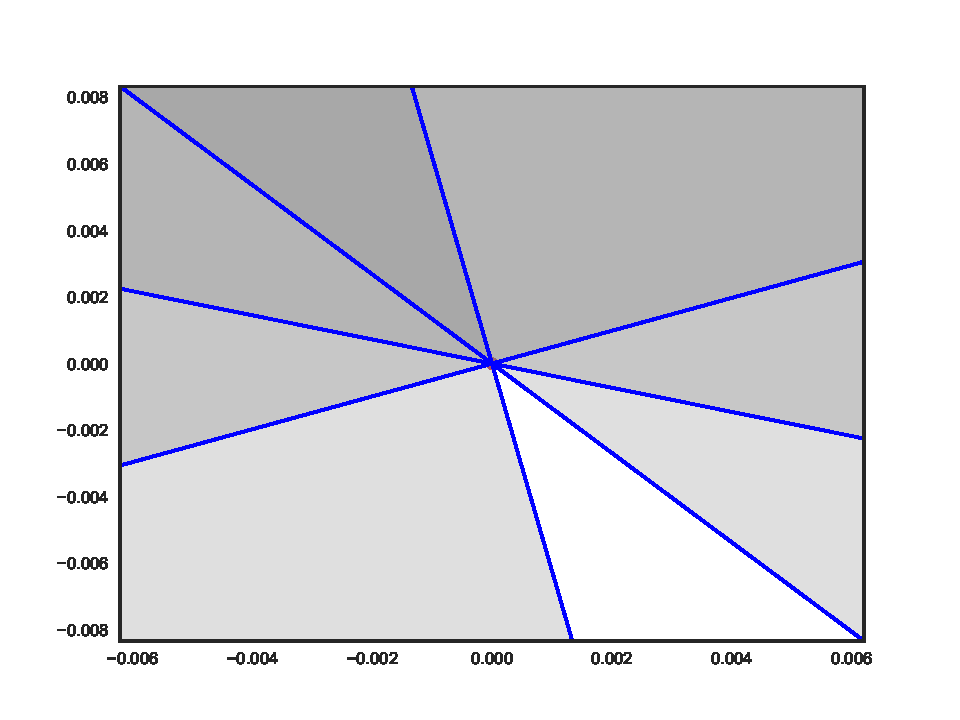
\includegraphics[width=\hsize]{img/toy/relu/conv2d_4-0.pdf}}
    %   \vskip1em
      \subcaptionbox{4th layer\label{fig:moonsReLU42}}{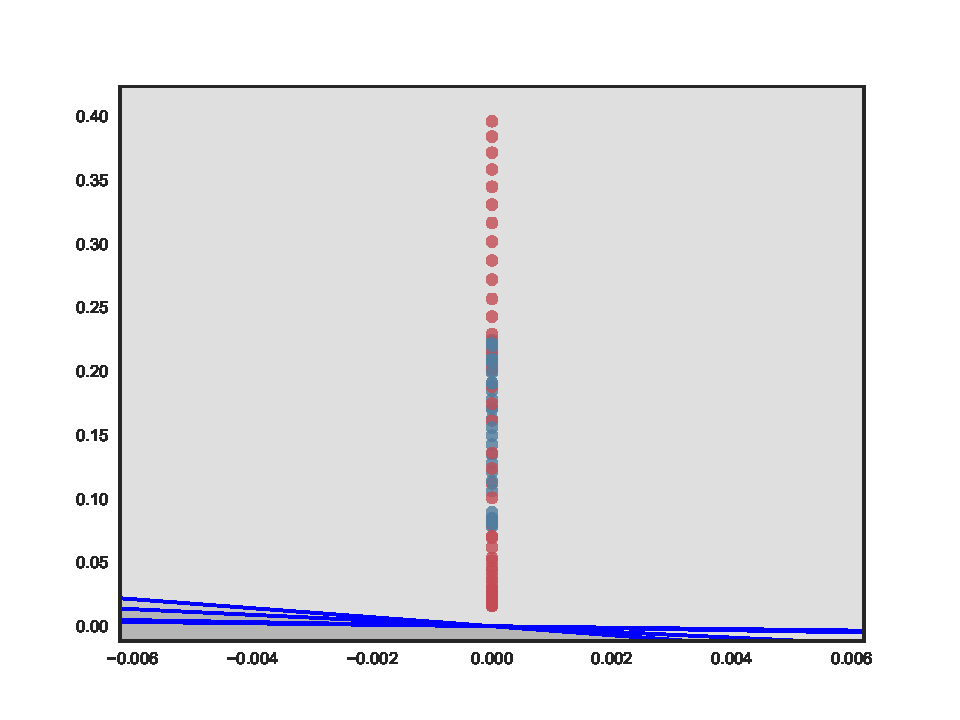
\includegraphics[width=\hsize]{img/toy/relu/conv2d_4-2.pdf}}
    }
    % \hskip1em
    \parbox{.195\textwidth}{%
      \subcaptionbox{25th layer\label{fig:moonsReLU251}}{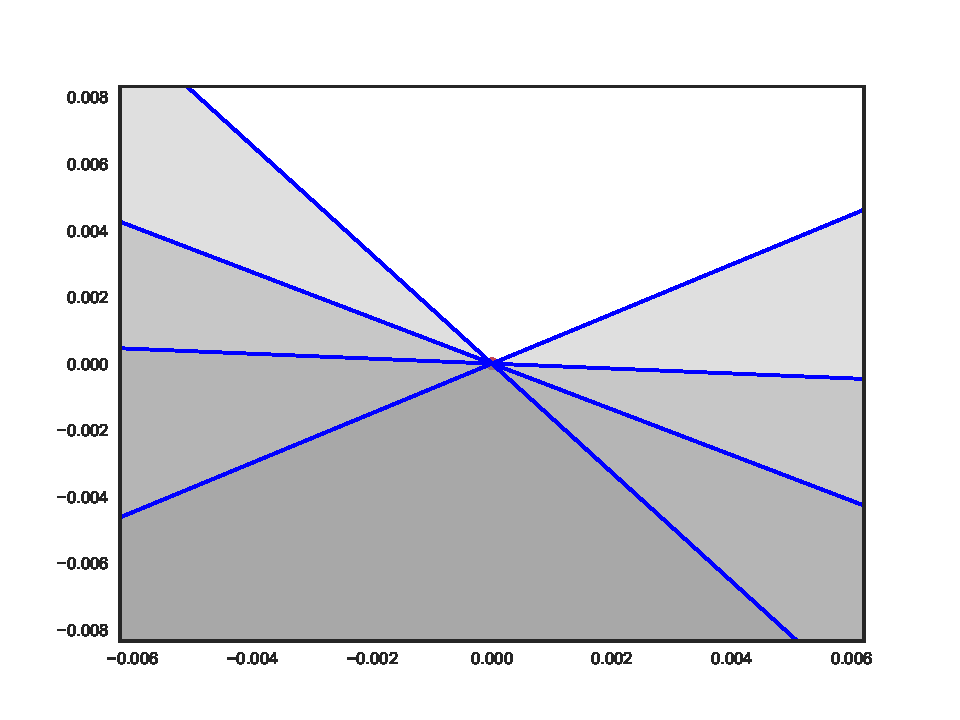
\includegraphics[width=\hsize]{img/toy/relu/conv2d_25-0.pdf}}
    %   \vskip1em
      \subcaptionbox{25th layer\label{fig:moonsReLU252}}{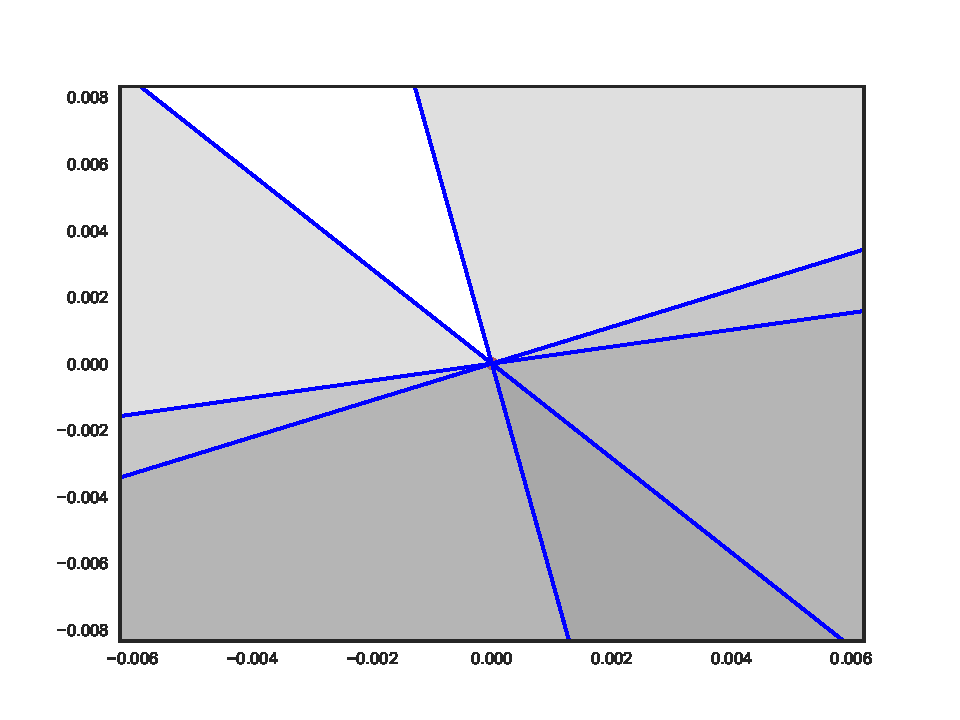
\includegraphics[width=\hsize]{img/toy/relu/conv2d_25-2.pdf}}
    }
    % \hskip1em
    \parbox{.195\textwidth}{%
      \subcaptionbox{Feature layer\label{fig:moonsReLUFeature1}}{\includegraphics[width=\hsize]{img/toy/relu/dense_1-0.pdf}}
    %   \vskip1em
      \subcaptionbox{Feature layer\label{fig:moonsReLUFeature2}}{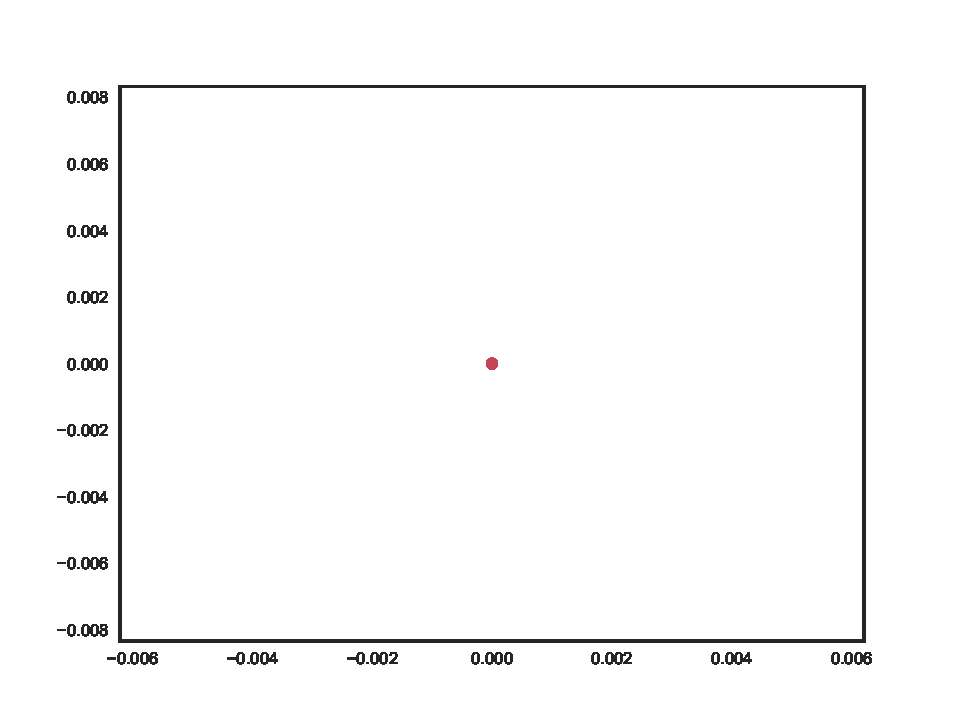
\includegraphics[width=\hsize]{img/toy/relu/dense_1-2.pdf}}
    }
    % \hskip1em
    \parbox{.195\textwidth}{%
      \subcaptionbox{Output\label{fig:moonsReLUOutput}}{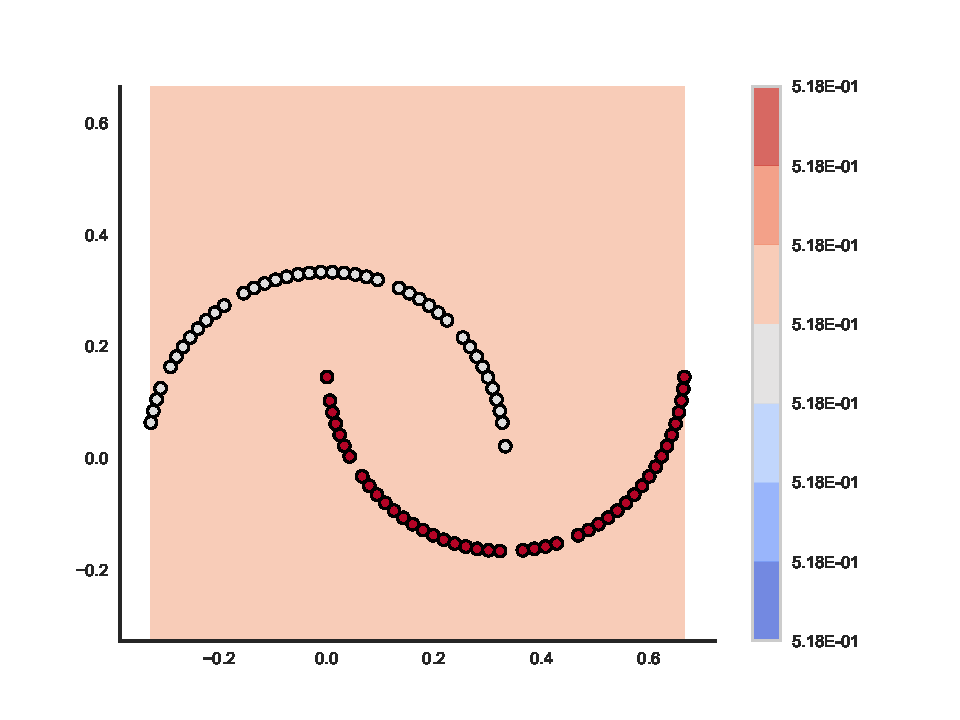
\includegraphics[width=\hsize]{img/toy/relu/output.pdf}}
    }
  }
  \caption{Data transformed across a 50x4 \ReLU classification network. Notice how the the dataset is progressively mapped to zero as it traverses the network. This renders the output layer unable to solve the problem.}
    \label{fig:moonsReLU}
\end{figure*}

\begin{figure*}
  \centering
  \parbox{\textwidth}{
    \parbox{.195\textwidth}{%
      \subcaptionbox{Input layer\label{fig:moonsReLUBNInput}}{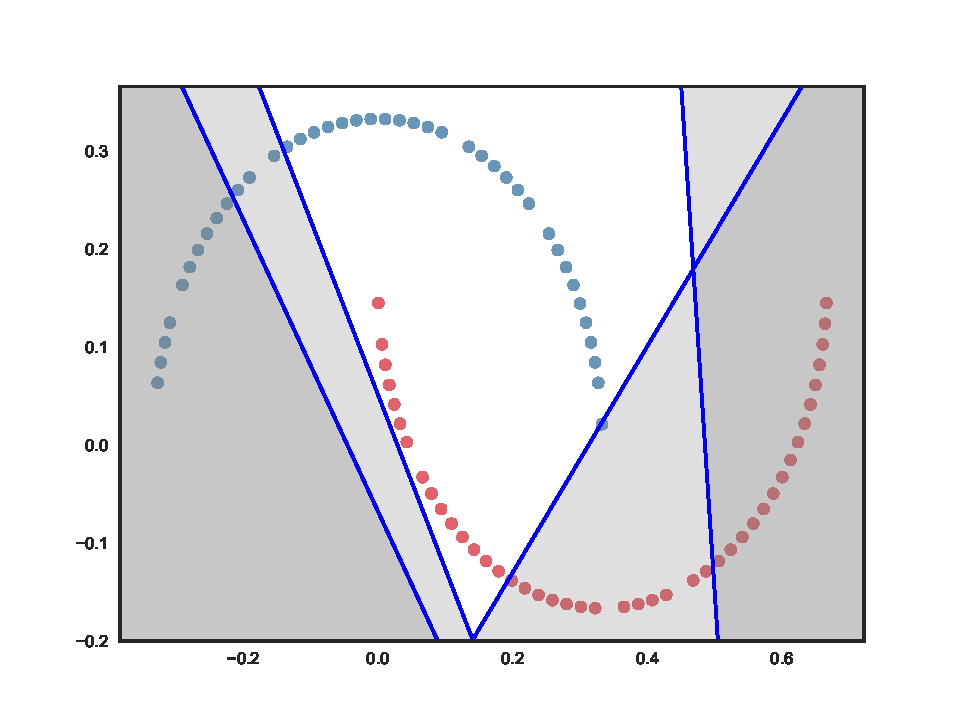
\includegraphics[width=\hsize]{img/toy/relu-bn/conv2d_1-0.pdf}}
    }
    % \hskip1em
    \parbox{.195\textwidth}{%
      \subcaptionbox{4th layer\label{fig:moonsReLUBN41}}{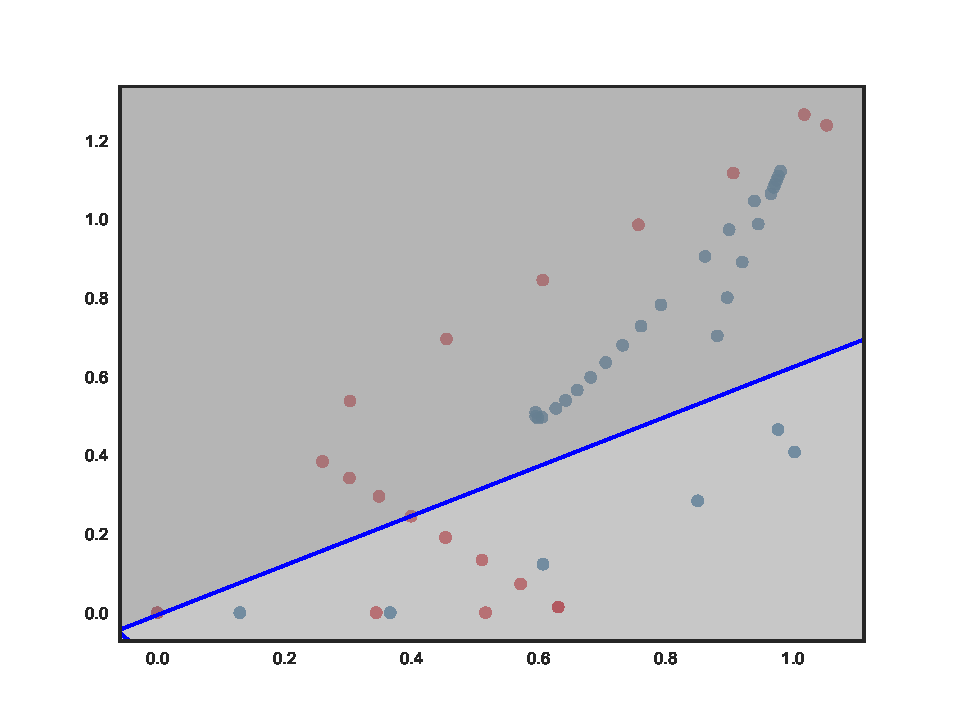
\includegraphics[width=\hsize]{img/toy/relu-bn/conv2d_4-0.pdf}}
    %   \vskip1em
      \subcaptionbox{4th layer\label{fig:moonsReLUBN42}}{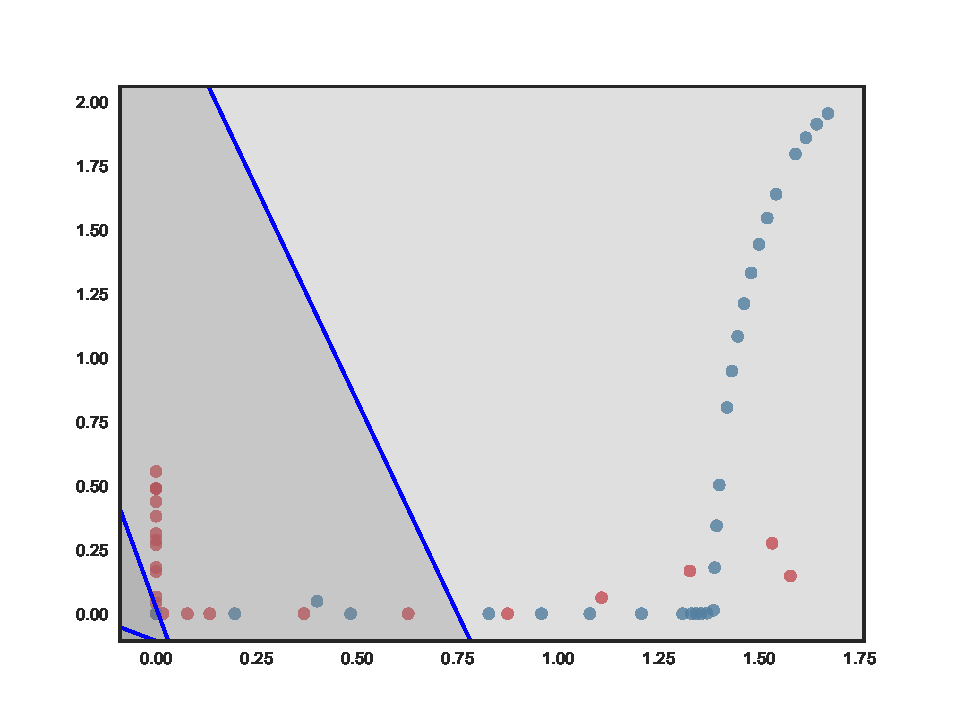
\includegraphics[width=\hsize]{img/toy/relu-bn/conv2d_4-2.pdf}}
    }
    % \hskip1em
    \parbox{.195\textwidth}{%
      \subcaptionbox{25th layer\label{fig:moonsReLUBN251}}{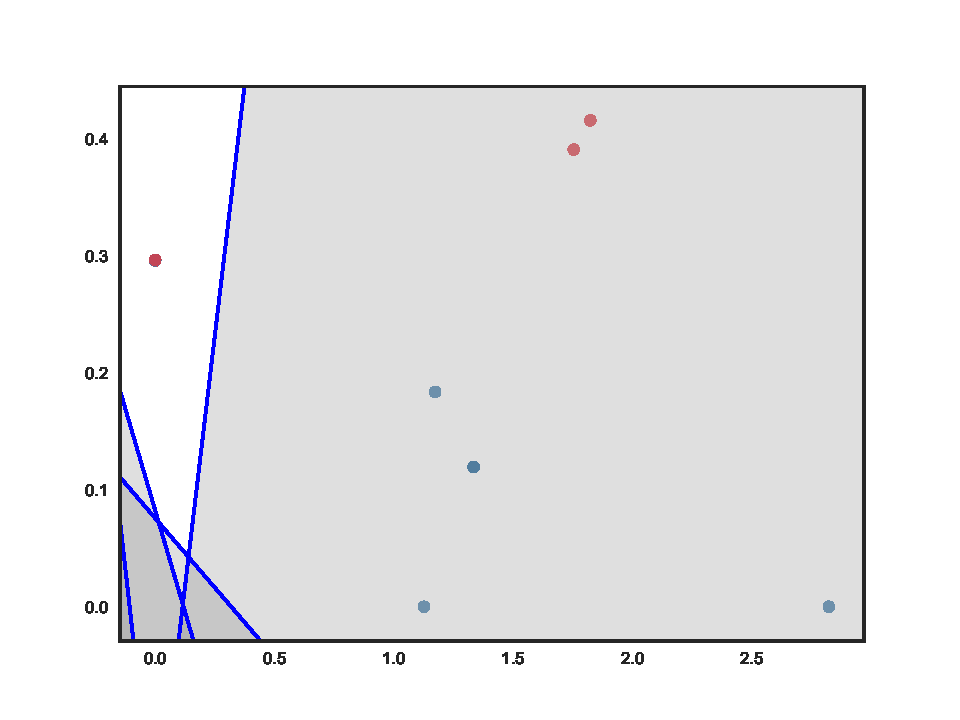
\includegraphics[width=\hsize]{img/toy/relu-bn/conv2d_25-0.pdf}}
    %   \vskip1em
      \subcaptionbox{25th layer\label{fig:moonsReLUBN252}}{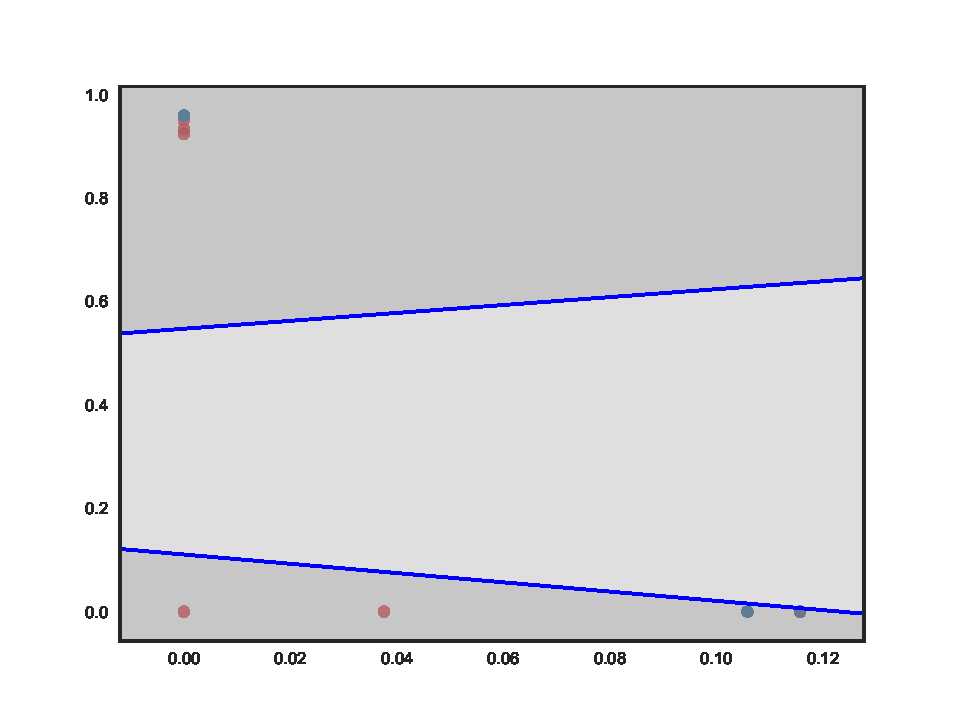
\includegraphics[width=\hsize]{img/toy/relu-bn/conv2d_25-2.pdf}} 
    }
    % \hskip1em
    \parbox{.195\textwidth}{%
      \subcaptionbox{Feature layer\label{fig:moonsReLUBNFeature1}}{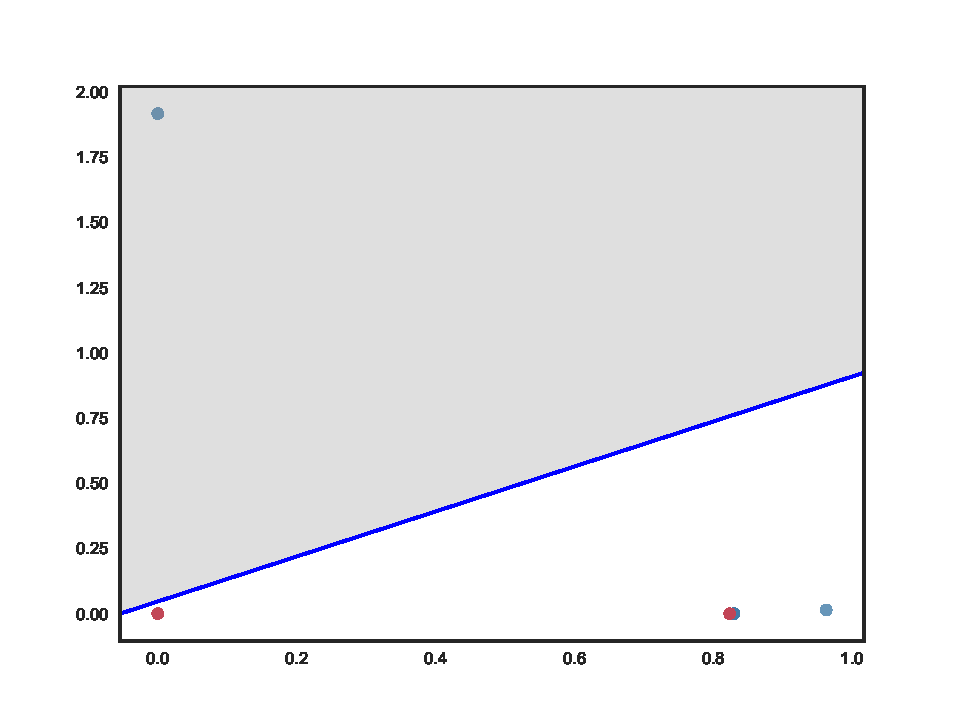
\includegraphics[width=\hsize]{img/toy/relu-bn/dense_1-0.pdf}}
    %   \vskip1em
      \subcaptionbox{Feature layer\label{fig:moonsReLUBNFeature2}}{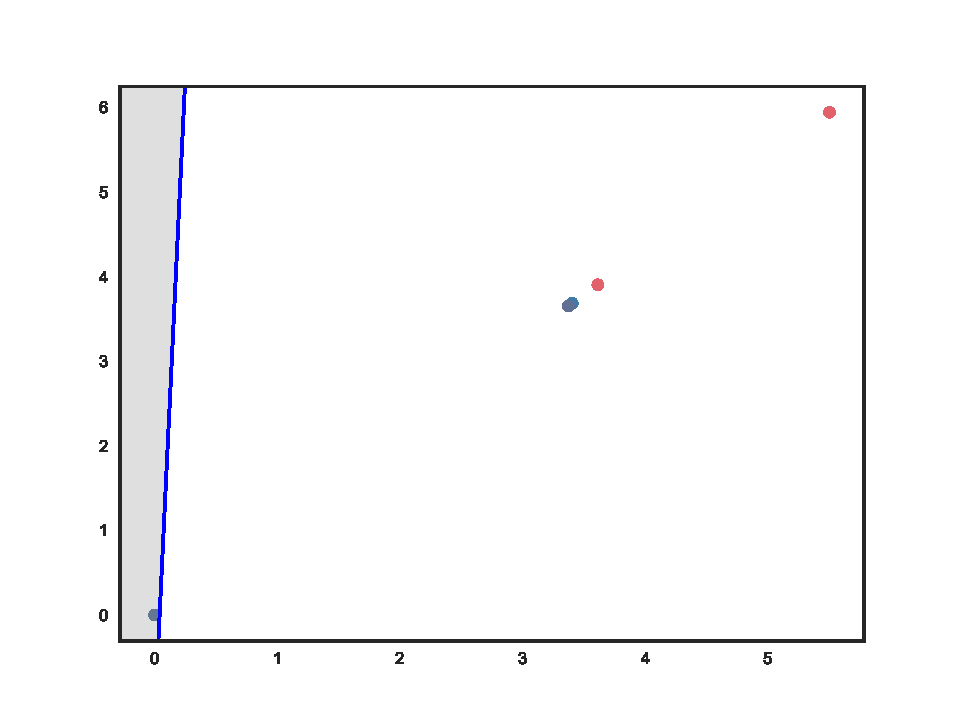
\includegraphics[width=\hsize]{img/toy/relu-bn/dense_1-2.pdf}} 
    }
    % \hskip1em
    \parbox{.195\textwidth}{%
      \subcaptionbox{Output\label{fig:moonsReLUBNOutput}}{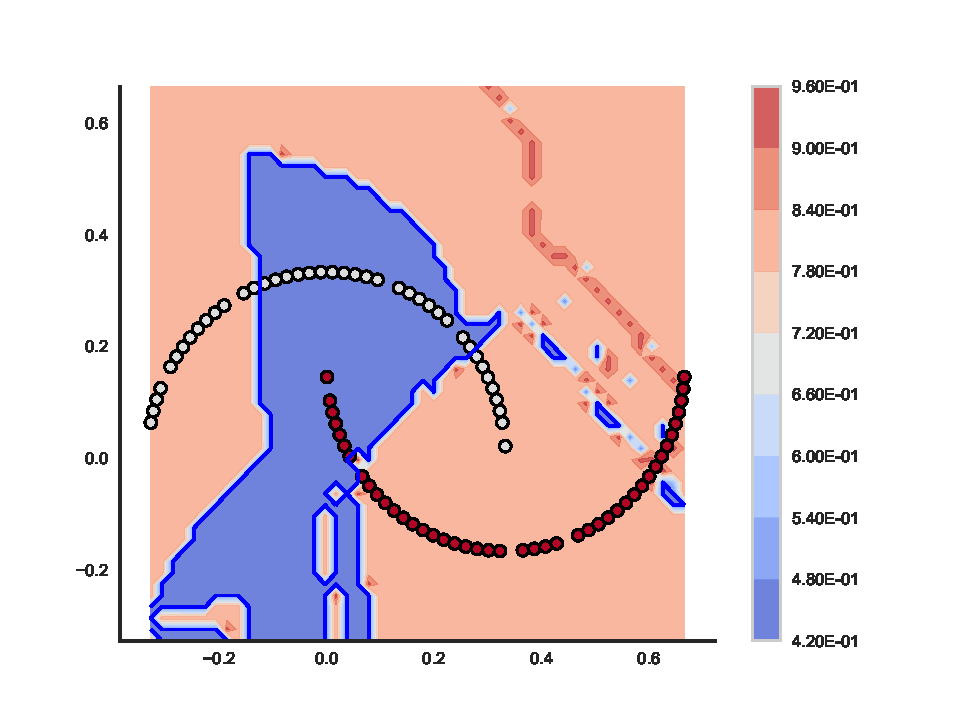
\includegraphics[width=\hsize]{img/toy/relu-bn/output.pdf}}
    }
  }
  \caption{Data transformed across a 50x4 \ReLUBN network. The dataset is collapsed in few points at the feature layer. As the gradient cannot be backpropagated across the truncation after the affine transform of $\gamma$ and $\beta$ despite the standarization, failing in the same manner than \ReLU only that with non-zero activations. This results in \emph{topological mixing} of the datasets. Therefore, the representational capability of the network is hindered to such extent that the resulting output, although non-trivial, is totally arbitrary.}
    \label{fig:moonsReLUBN}
\end{figure*}


\begin{figure*}
  \centering
     % Unitwise
  \parbox{\textwidth}{
    \parbox{.195\textwidth}{%
      \subcaptionbox{Input layer\label{fig:moonsUnitwiseInput}}{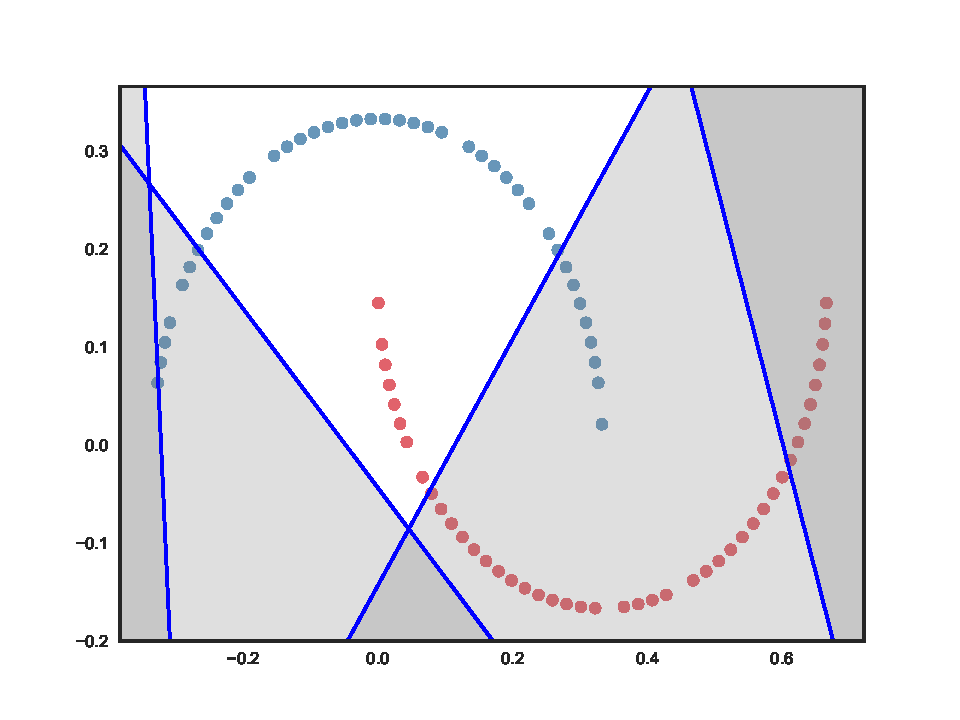
\includegraphics[width=\hsize]{img/toy/unitwise/conv2d_1-0.pdf}}
    }
    % \hskip1em
    \parbox{.195\textwidth}{%
      \subcaptionbox{4th layer\label{fig:moonsUnitwise41}}{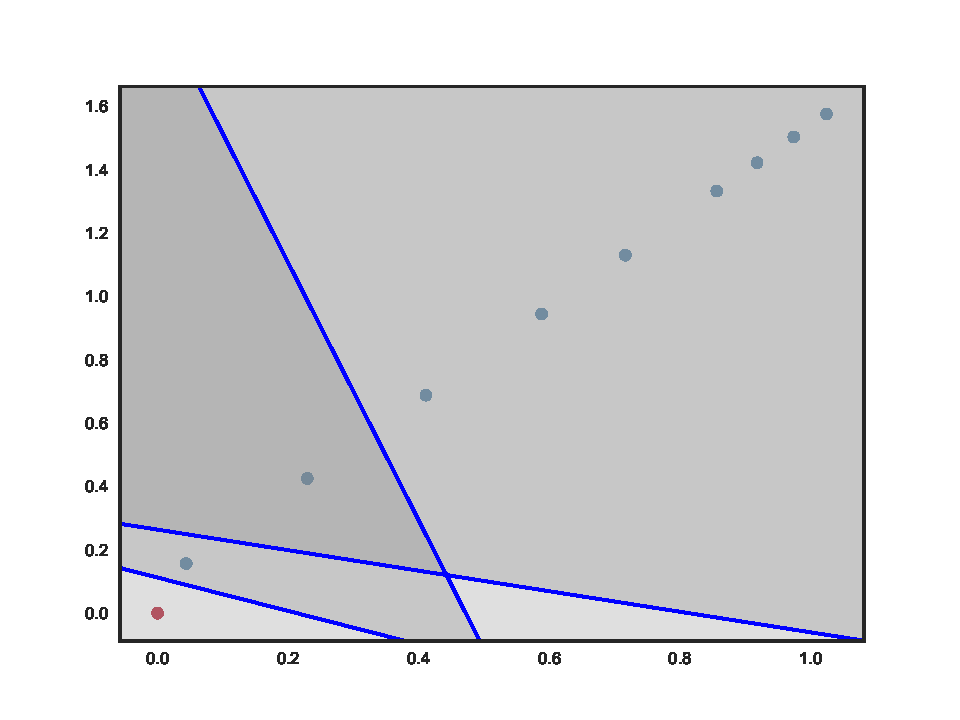
\includegraphics[width=\hsize]{img/toy/unitwise/conv2d_4-0.pdf}}
    %   \vskip1em
      \subcaptionbox{4th layer\label{fig:moonsUnitwise42}}{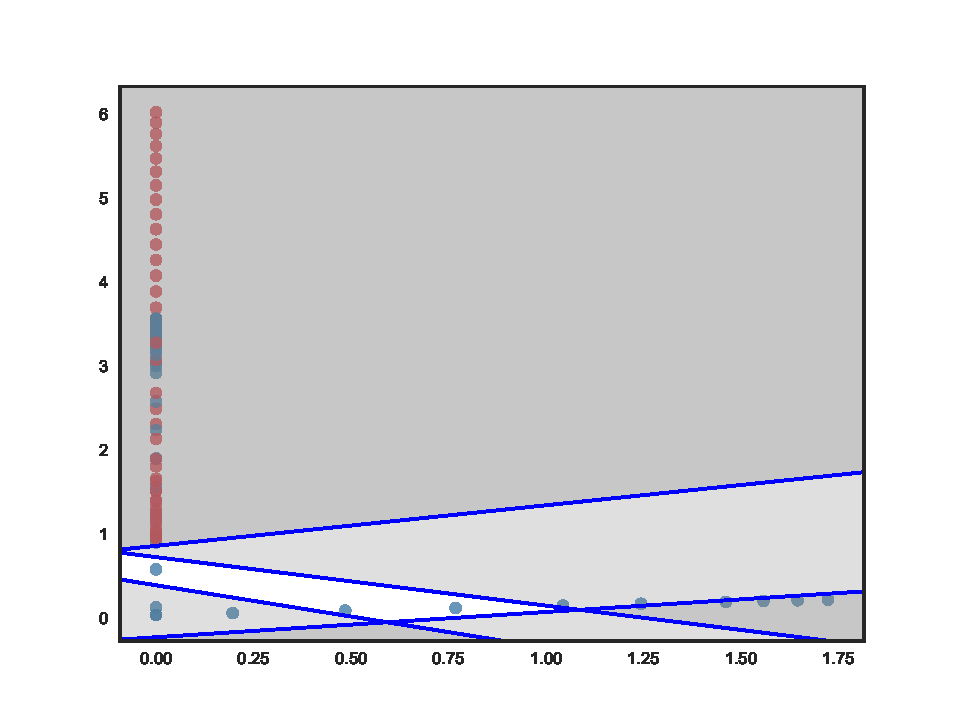
\includegraphics[width=\hsize]{img/toy/unitwise/conv2d_4-2.pdf}}
    }
    % \hskip1em
    \parbox{.195\textwidth}{%
      \subcaptionbox{25th layer\label{fig:moonsUnitwise251}}{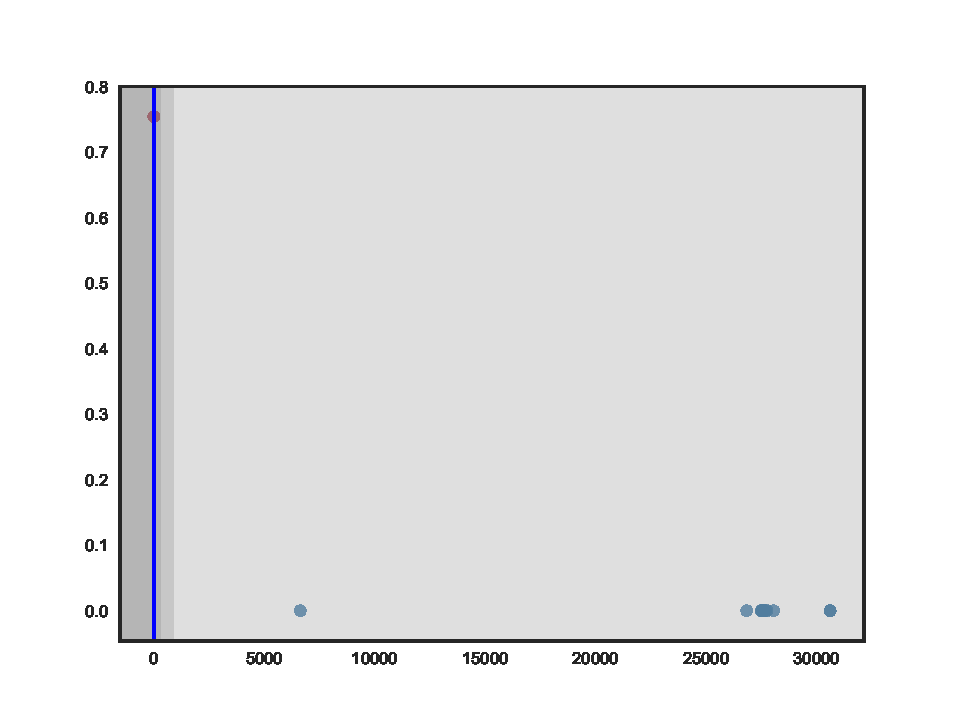
\includegraphics[width=\hsize]{img/toy/unitwise/conv2d_25-0.pdf}}
    %   \vskip1em
      \subcaptionbox{25th layer\label{fig:moonsUnitwise252}}{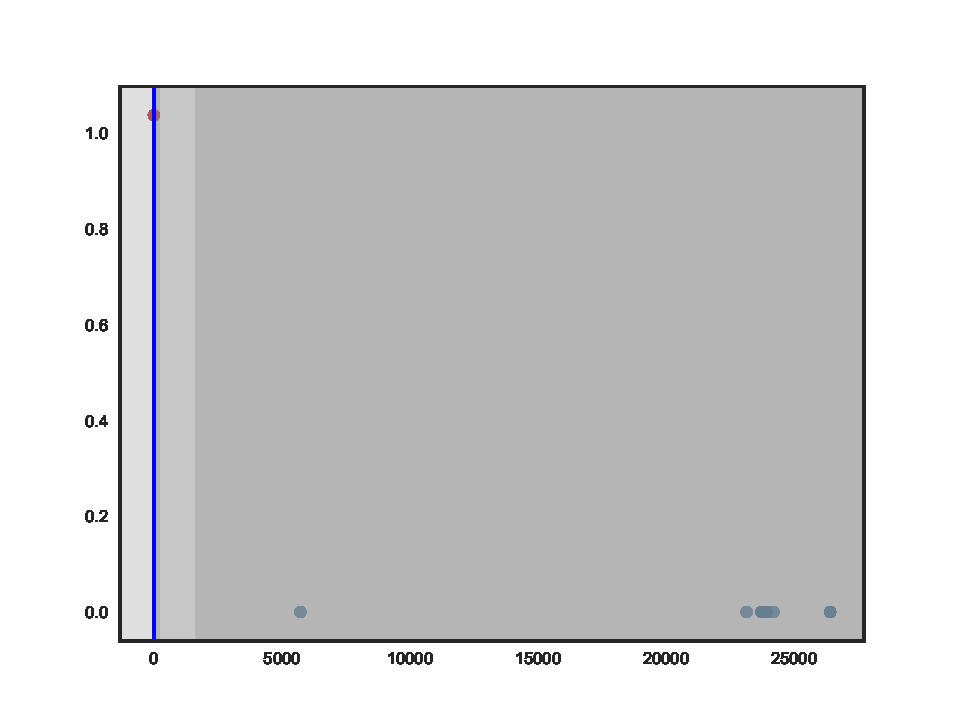
\includegraphics[width=\hsize]{img/toy/unitwise/conv2d_25-2.pdf}}
    }
    % \hskip1em
    \parbox{.195\textwidth}{%
      \subcaptionbox{Feature layer\label{fig:moonsUnitwiseFeature1}}{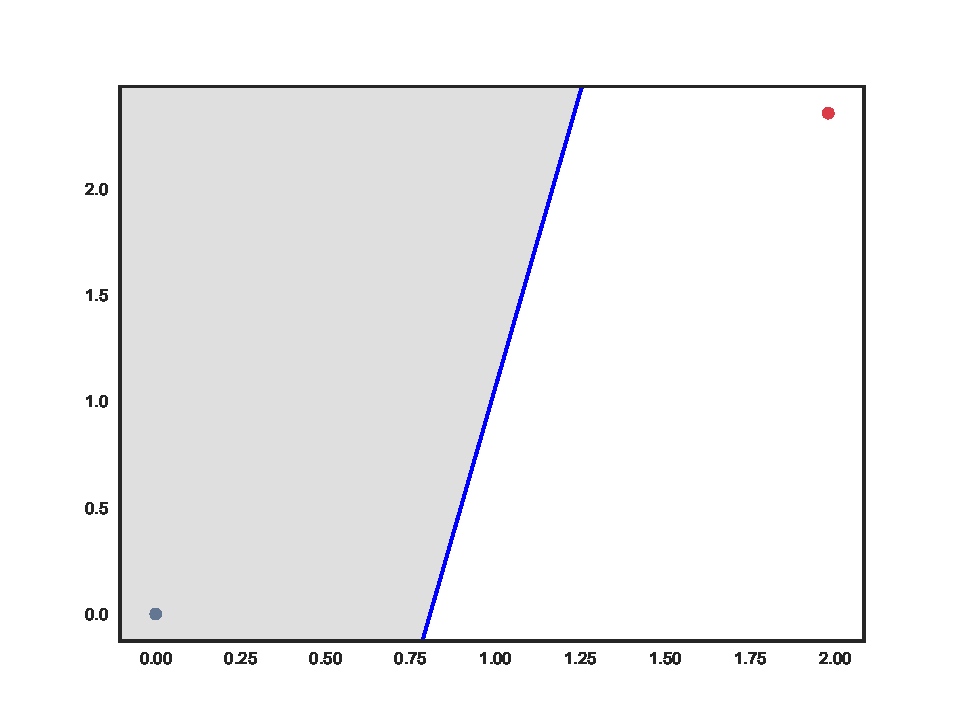
\includegraphics[width=\hsize]{img/toy/unitwise/dense_1-0.pdf}}
    %   \vskip1em
      \subcaptionbox{Feature layer\label{fig:moonsUnitwiseFeature2}}{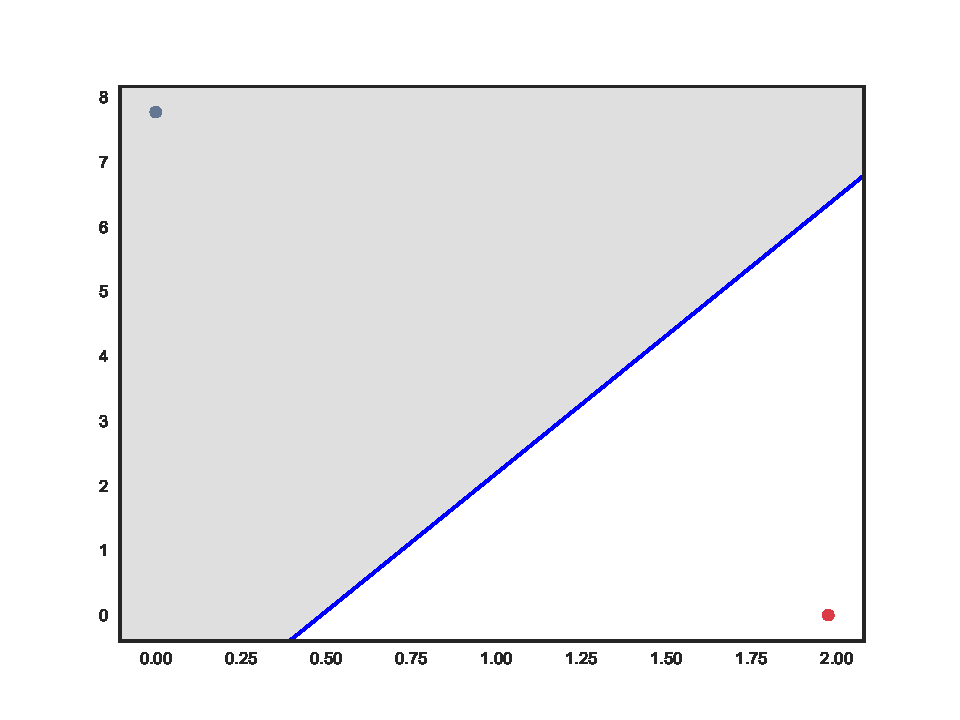
\includegraphics[width=\hsize]{img/toy/unitwise/dense_1-2.pdf}}
    }
    % \hskip1em
    \parbox{.195\textwidth}{%
      \subcaptionbox{Output\label{fig:moonsUnitwiseOutput}}{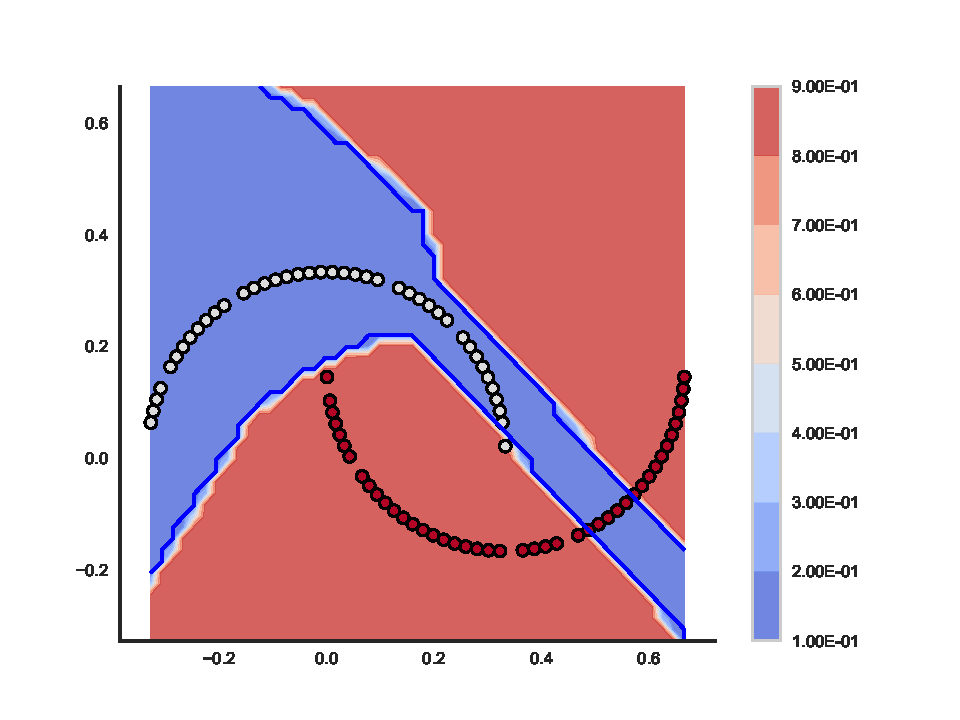
\includegraphics[width=\hsize]{img/toy/unitwise/output.pdf}}
    }
  }
  \caption{Data transformed across a 50x4 \SepUnit network. Notice how dead and affine units have been reduced. Despite collapsing the dataset in two points at the feature layer, the classification performed in the output layer is approximately correct. We conjecture that this is due the dead point addressed with \SepPoint.}
    \label{fig:moonsUnitwise}
\end{figure*}



\begin{figure*}
  \centering
  %Pointwise
  \parbox{\textwidth}{
    \parbox{.195\textwidth}{%
      \subcaptionbox{Input layer\label{fig:moonsPointwiseInput}}{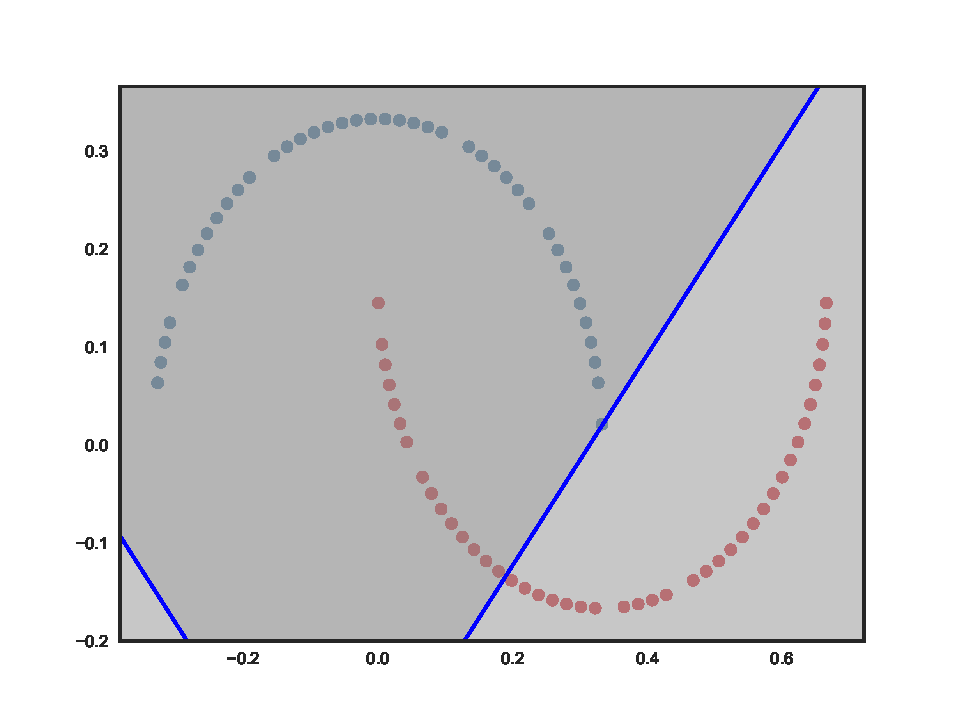
\includegraphics[width=\hsize]{img/toy/pointwise/conv2d_1-0.pdf}}
    }
    % \hskip1em
    \parbox{.195\textwidth}{%
      \subcaptionbox{4th layer\label{fig:moonsPointwise41}}{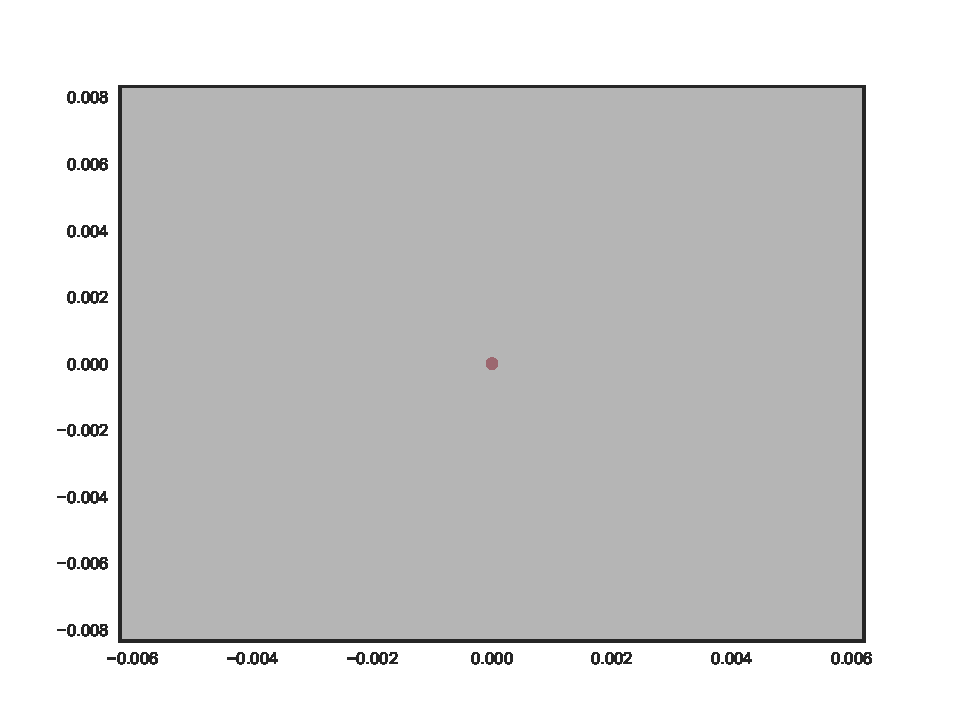
\includegraphics[width=\hsize]{img/toy/pointwise/conv2d_4-0.pdf}}
    %   \vskip1em
      \subcaptionbox{4th layer\label{fig:moonsPointwise42}}{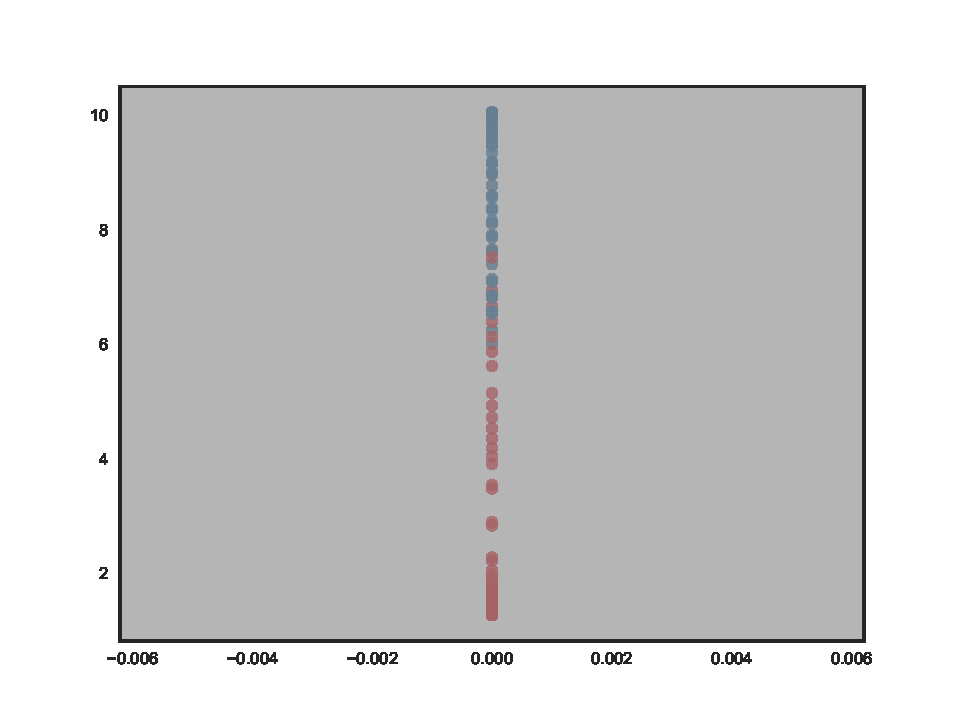
\includegraphics[width=\hsize]{img/toy/pointwise/conv2d_4-2.pdf}} 
    }
    % \hskip1em
    \parbox{.195\textwidth}{%
      \subcaptionbox{25th layer\label{fig:moonsPointwise251}}{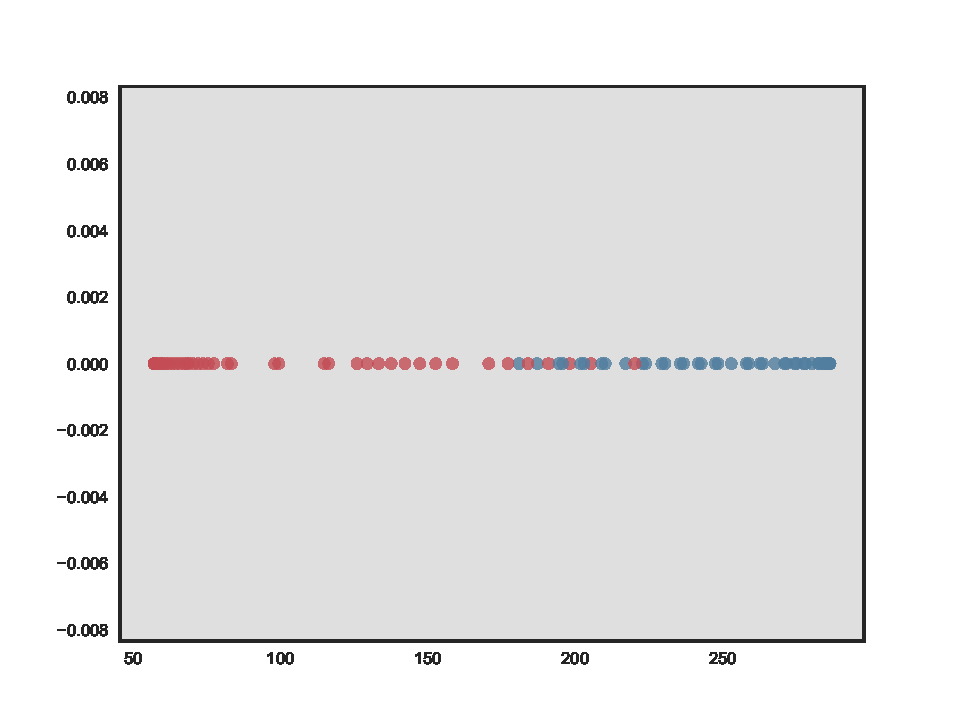
\includegraphics[width=\hsize]{img/toy/pointwise/conv2d_25-0.pdf}}
    %   \vskip1em
      \subcaptionbox{25th layer\label{fig:moonsPointwise252}}{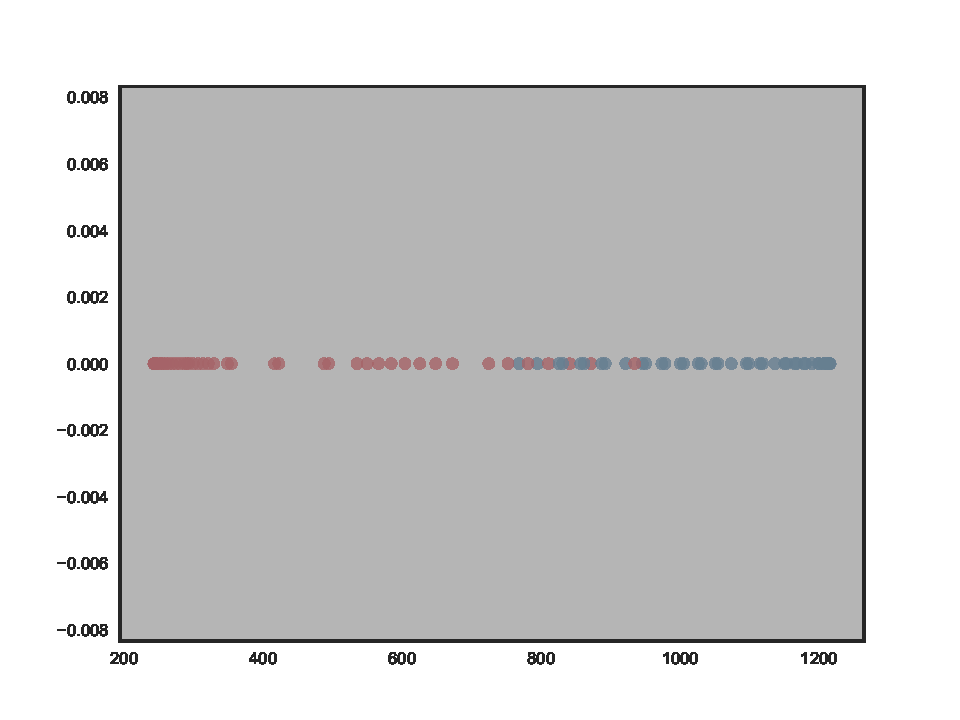
\includegraphics[width=\hsize]{img/toy/pointwise/conv2d_25-2.pdf}} 
    }
    % \hskip1em
    \parbox{.195\textwidth}{%
      \subcaptionbox{Feature layer\label{fig:moonsPointwiseFeature1}}{\includegraphics[width=\hsize]{img/toy/pointwise/dense_1-0.pdf}}
    %   \vskip1em
      \subcaptionbox{Feature layer\label{fig:moonsPointwiseFeature2}}{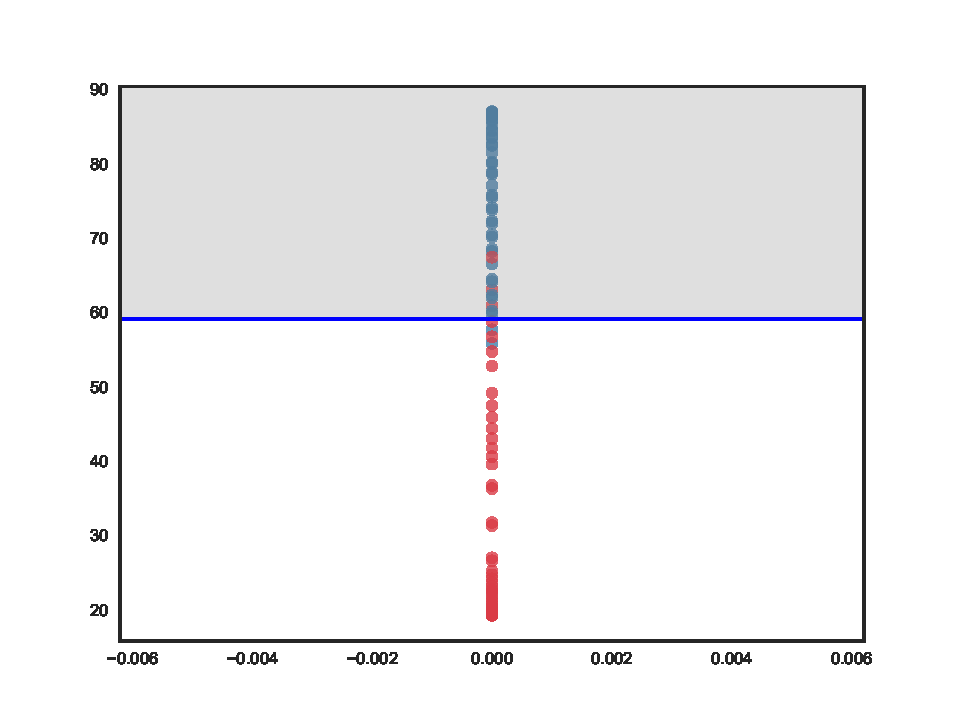
\includegraphics[width=\hsize]{img/toy/pointwise/dense_1-2.pdf}} 
    }
    % \hskip1em
    \parbox{.195\textwidth}{%
      \subcaptionbox{Output\label{fig:moonsPointwiseOutput}}{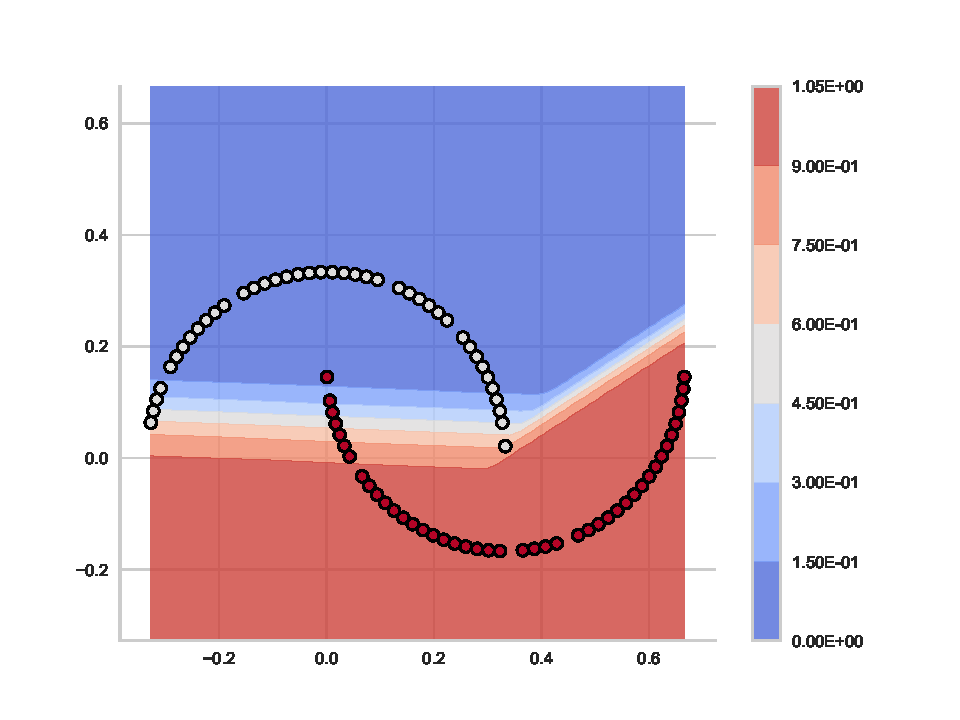
\includegraphics[width=\hsize]{img/toy/pointwise/output.pdf}}
    }
  }
  \caption{Data transformed across a 50x4 \SepPoint network. The network displays a richer internal representation without collapsing the dataset like \SepUnit or \ReLUBN. However, plenty of dead and affine units appear since they are not penalized, causing underfitting.}
    \label{fig:moonsPointwise}
\end{figure*}


\begin{figure*}
  \centering
   \parbox{\textwidth}{
    \parbox{.195\textwidth}{%
      \subcaptionbox{Input layer\label{fig:moonsUnitpointwiseInput}}{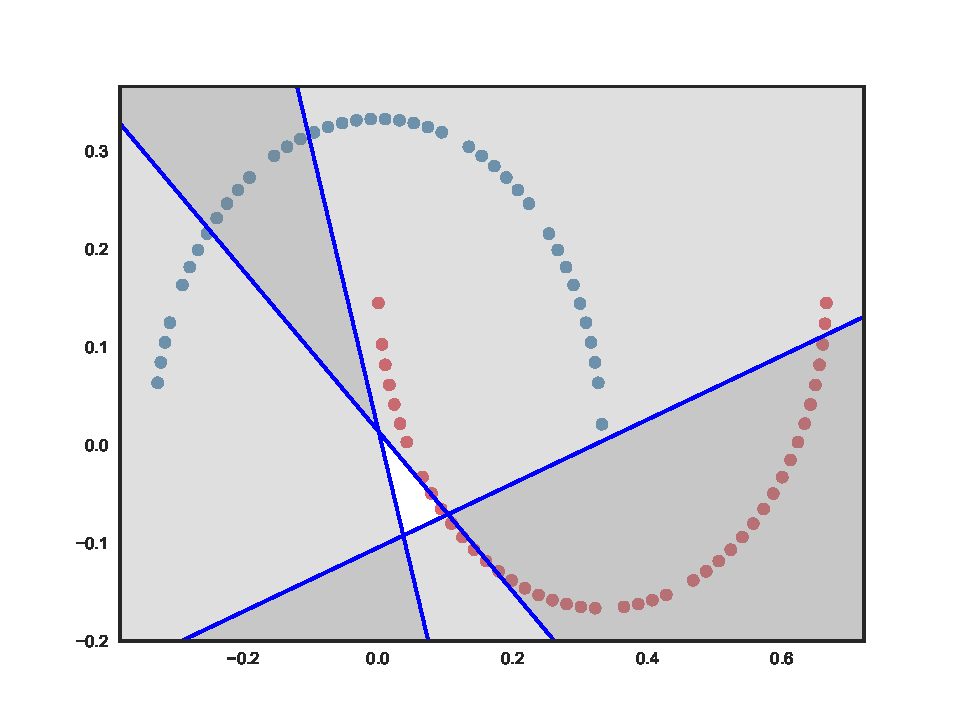
\includegraphics[width=\hsize]{img/toy/unitpointwise/conv2d_1-0.pdf}}
    }
    % \hskip1em
    \parbox{.195\textwidth}{%
      \subcaptionbox{4th layer\label{fig:moonsUnitpointwise41}}{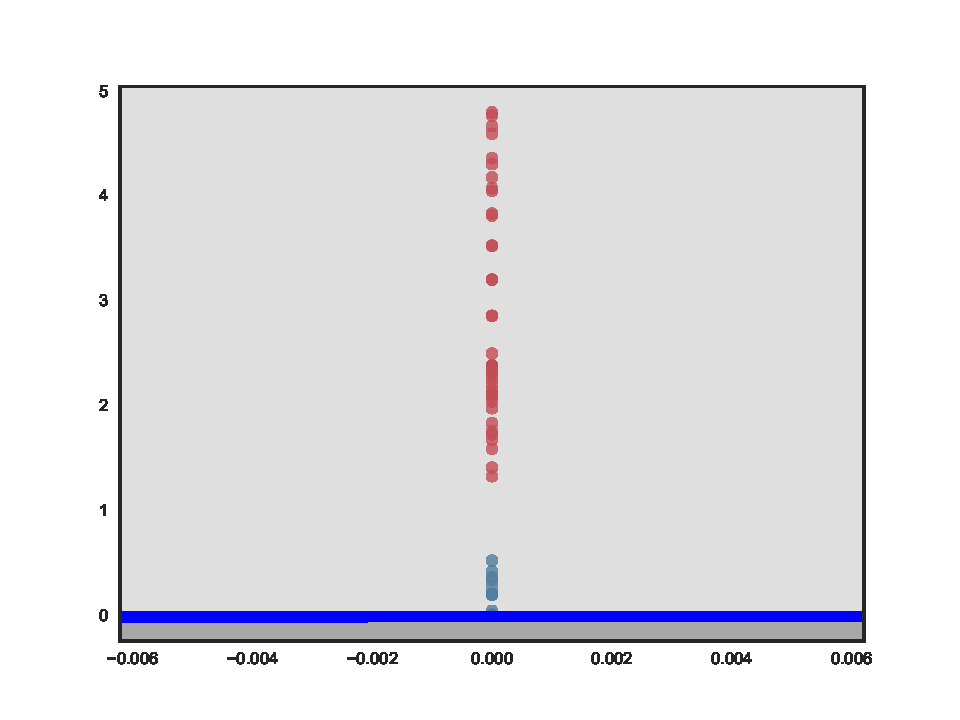
\includegraphics[width=\hsize]{img/toy/unitpointwise/conv2d_4-0.pdf}}
    %   \vskip1em
      \subcaptionbox{4th layer\label{fig:moonsUnitpointwise42}}{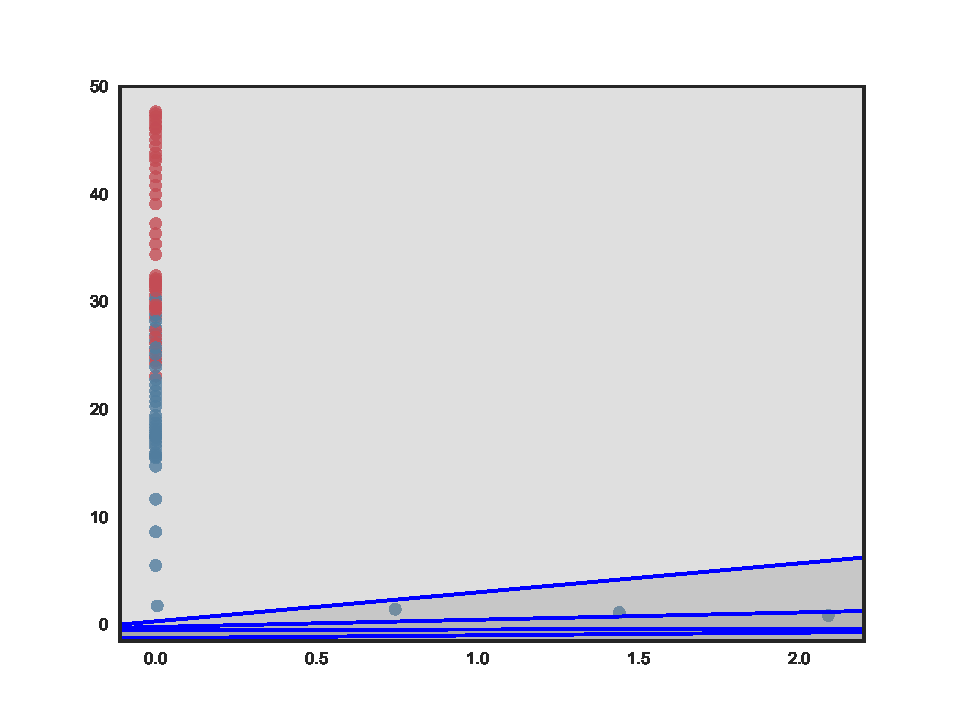
\includegraphics[width=\hsize]{img/toy/unitpointwise/conv2d_4-2.pdf}} 
    }
    % \hskip1em
    \parbox{.195\textwidth}{%
      \subcaptionbox{25th layer\label{fig:moonsUnitpointwise251}}{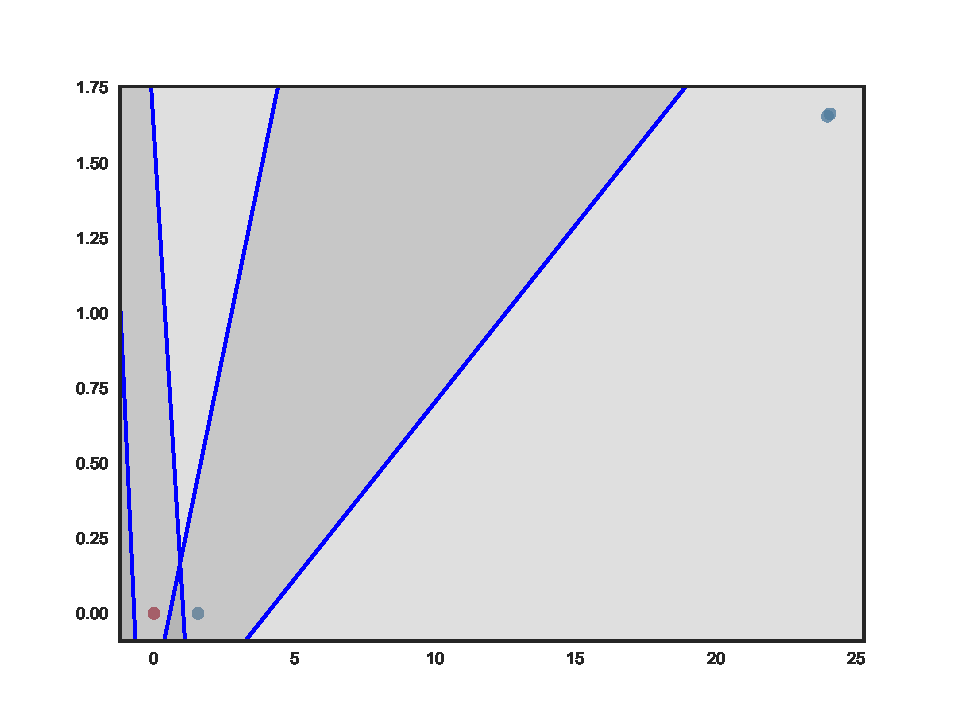
\includegraphics[width=\hsize]{img/toy/unitpointwise/conv2d_25-0.pdf}}
    %   \vskip1em
      \subcaptionbox{25th layer\label{fig:moonsUnitpointwise252}}{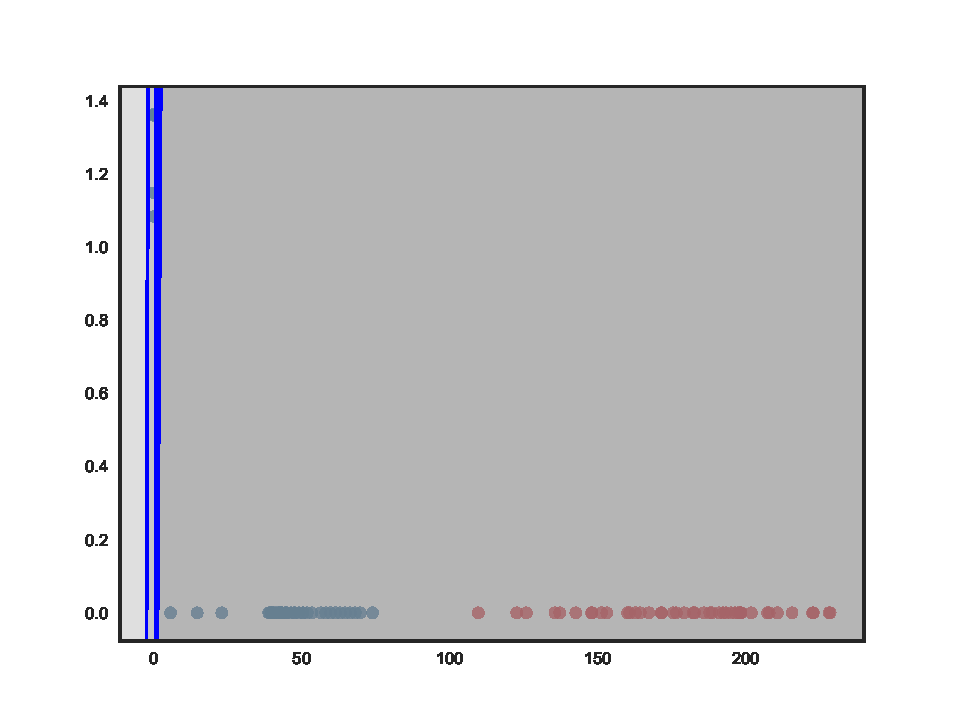
\includegraphics[width=\hsize]{img/toy/unitpointwise/conv2d_25-2.pdf}} 
    }
    % \hskip1em
    \parbox{.195\textwidth}{%
      \subcaptionbox{Feature layer\label{fig:moonsUnitpointwiseFeature1}}{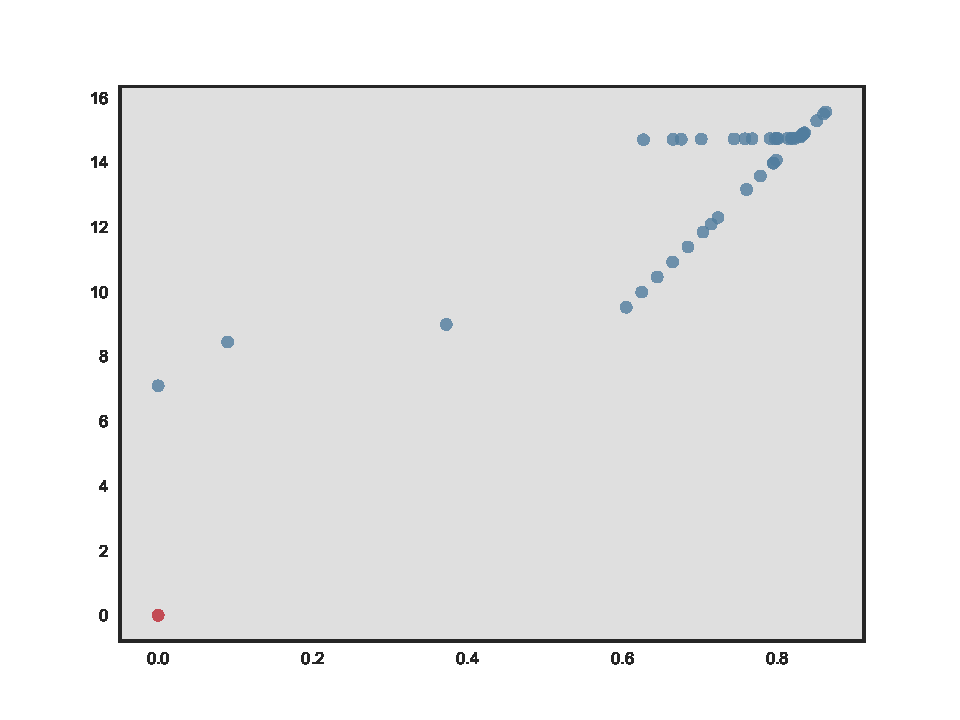
\includegraphics[width=\hsize]{img/toy/unitpointwise/dense_1-0.pdf}}
    %   \vskip1em
      \subcaptionbox{Feature layer\label{fig:moonsUnitpointwiseFeature2}}{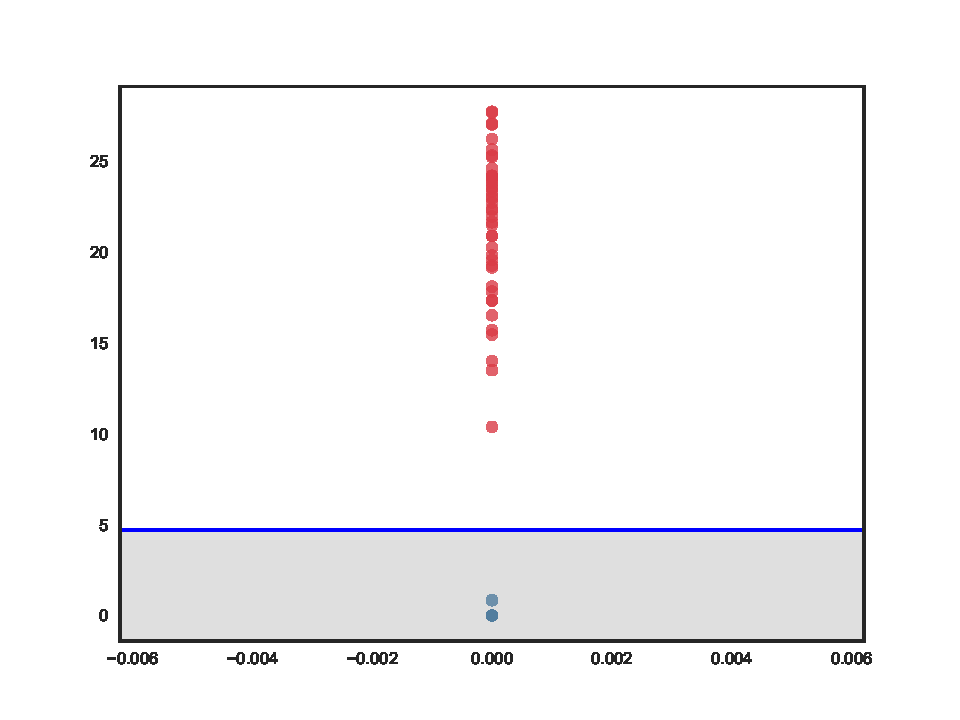
\includegraphics[width=\hsize]{img/toy/unitpointwise/dense_1-2.pdf}} 
    }
    % \hskip1em
    \parbox{.195\textwidth}{%
      \subcaptionbox{Output\label{fig:moonsUnitpointwiseOutput}}{
      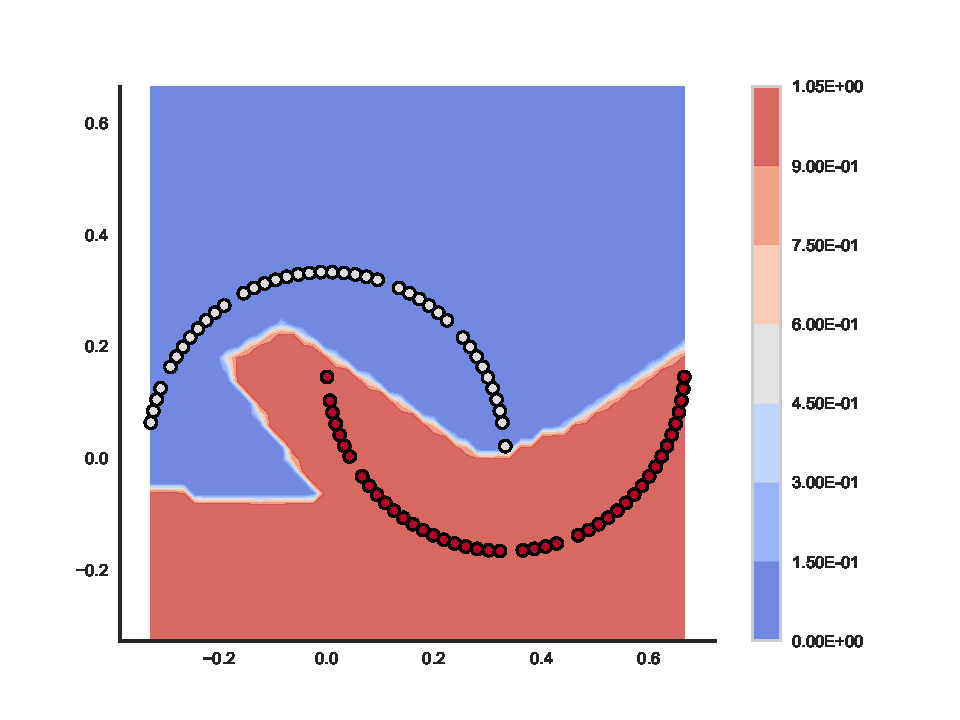
\includegraphics[clip, trim=2.35cm 1.75cm 4.5cm 0cm,width=\hsize, height=\hsize]{img/toy/unitpointwise/output.pdf}
      }
    }
  }

    \caption{Data transformed across a 50x4 \SepUnitPoint network. The network displays internal representations without collapsing the dataset like \SepPoint while retaining classification power like \SepUnit.}
    \label{fig:moonsUnitPointwise}
\end{figure*}

\begin{figure*}
  \centering
  \parbox{\textwidth}{
    \parbox{.195\textwidth}{%
      \subcaptionbox{Input layer\label{fig:moonsLayerwiseInput}}{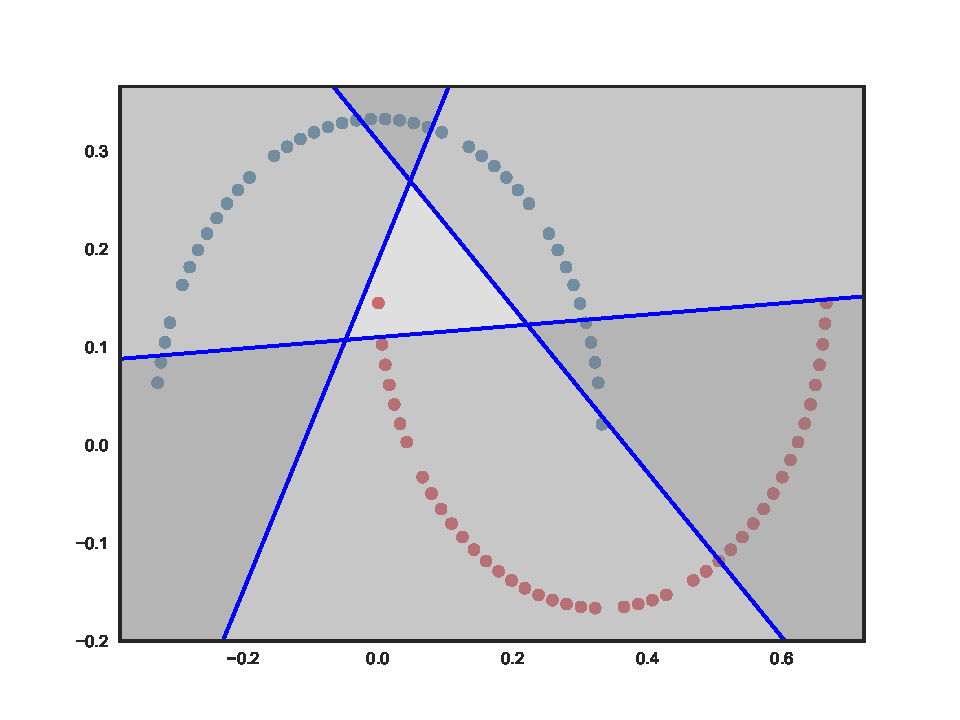
\includegraphics[width=\hsize]{img/toy/layerwise/conv2d_1-0.pdf}}
    }
    % \hskip1em
    \parbox{.195\textwidth}{%
      \subcaptionbox{4th layer\label{fig:moonsLayerwise41}}{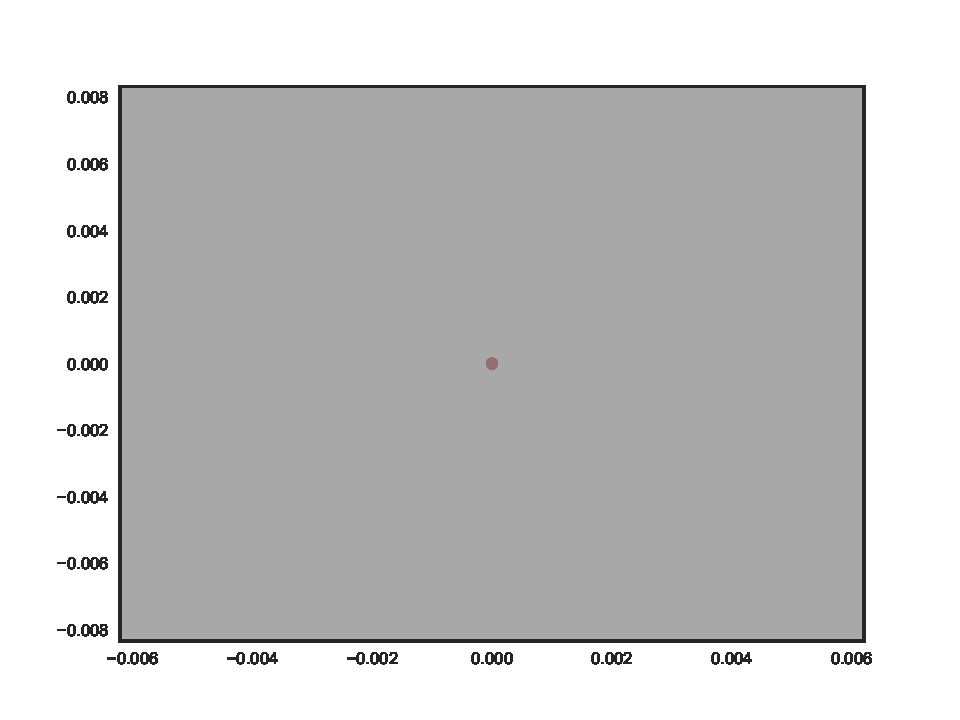
\includegraphics[width=\hsize]{img/toy/layerwise/conv2d_4-0.pdf}}
    %   \vskip1em
      \subcaptionbox{4th layer\label{fig:moonsLayerwise42}}{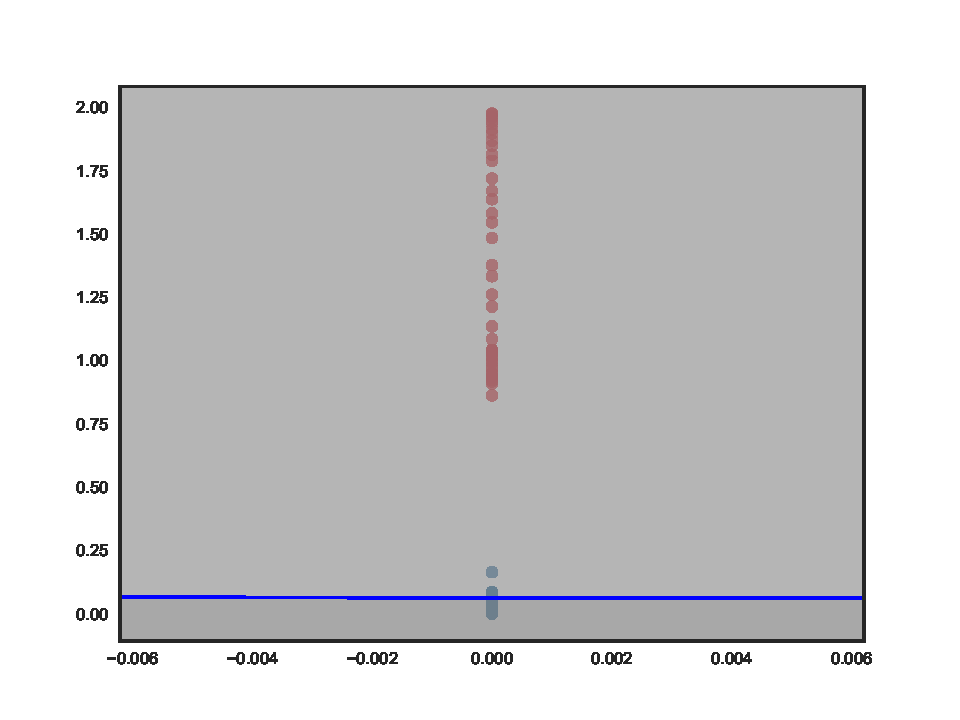
\includegraphics[width=\hsize]{img/toy/layerwise/conv2d_4-2.pdf}} 
    }
    % \hskip1em
    \parbox{.195\textwidth}{%
      \subcaptionbox{25th layer\label{fig:moonsLayerwise251}}{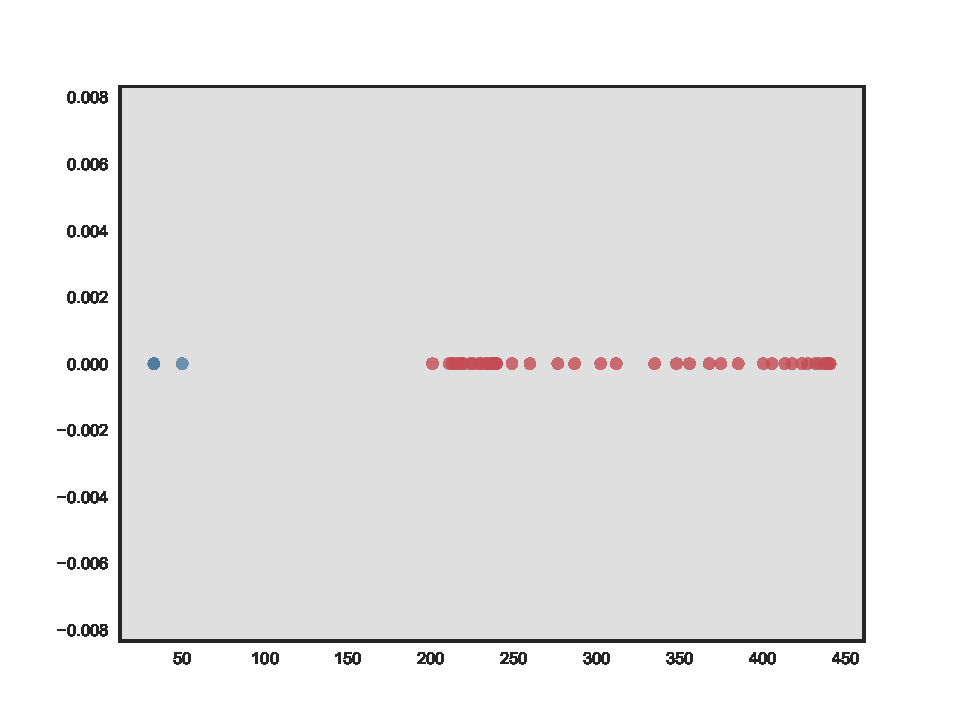
\includegraphics[width=\hsize]{img/toy/layerwise/conv2d_25-0.pdf}}
    %   \vskip1em
      \subcaptionbox{25th layer\label{fig:moonsLayerwise252}}{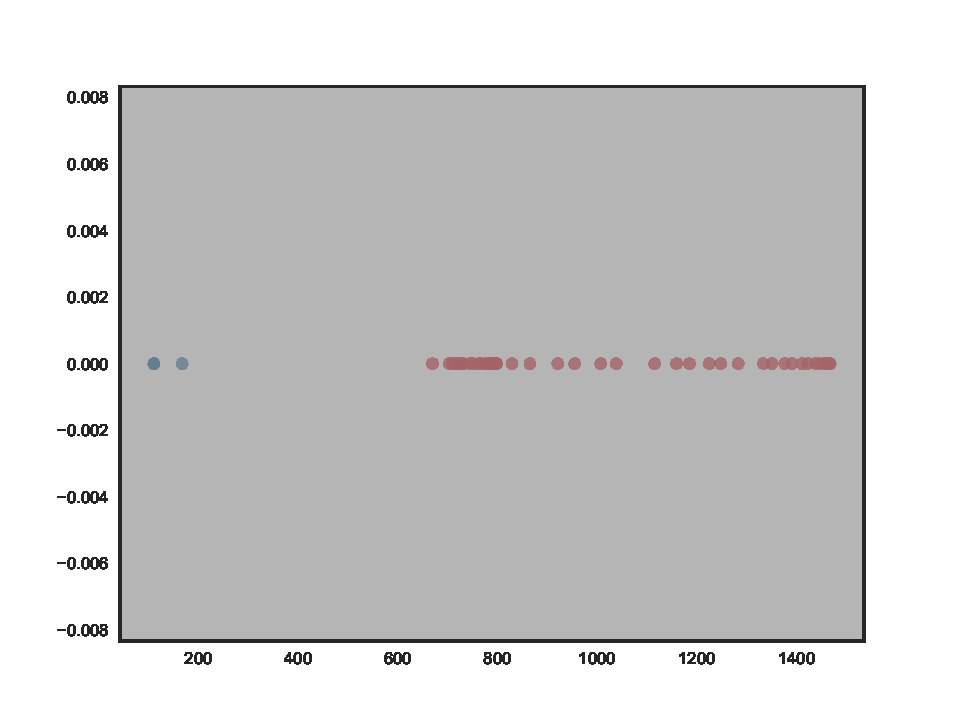
\includegraphics[width=\hsize]{img/toy/layerwise/conv2d_25-2.pdf}} 
    }
    % \hskip1em
    \parbox{.195\textwidth}{%
      \subcaptionbox{Feature layer\label{fig:moonsLayerwiseFeature1}}{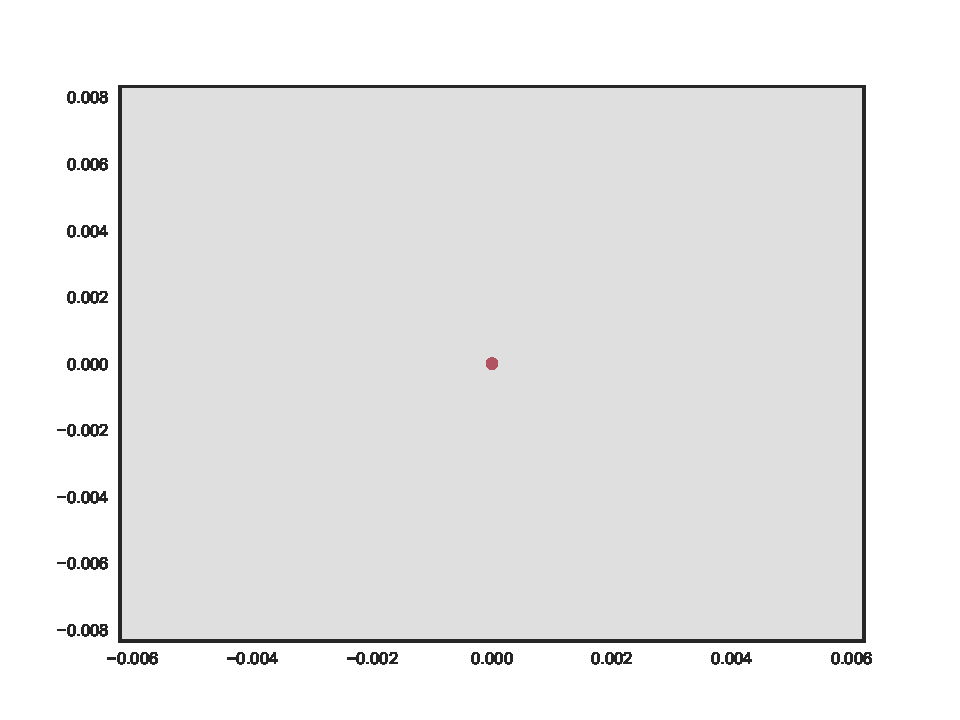
\includegraphics[width=\hsize]{img/toy/layerwise/dense_1-0.pdf}}
    %   \vskip1em
      \subcaptionbox{Feature layer\label{fig:moonsLayerwiseFeature2}}{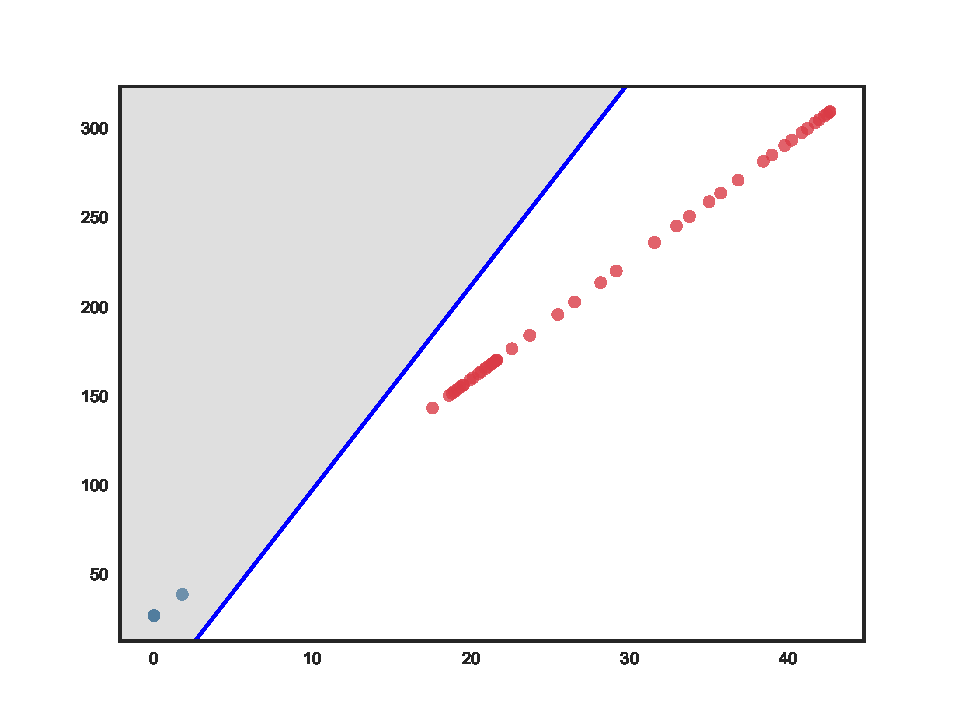
\includegraphics[width=\hsize]{img/toy/layerwise/dense_1-2.pdf}} 
    }
    % \hskip1em
    \parbox{.195\textwidth}{%
      \subcaptionbox{Output\label{fig:moonsLayerwiseOutput}}{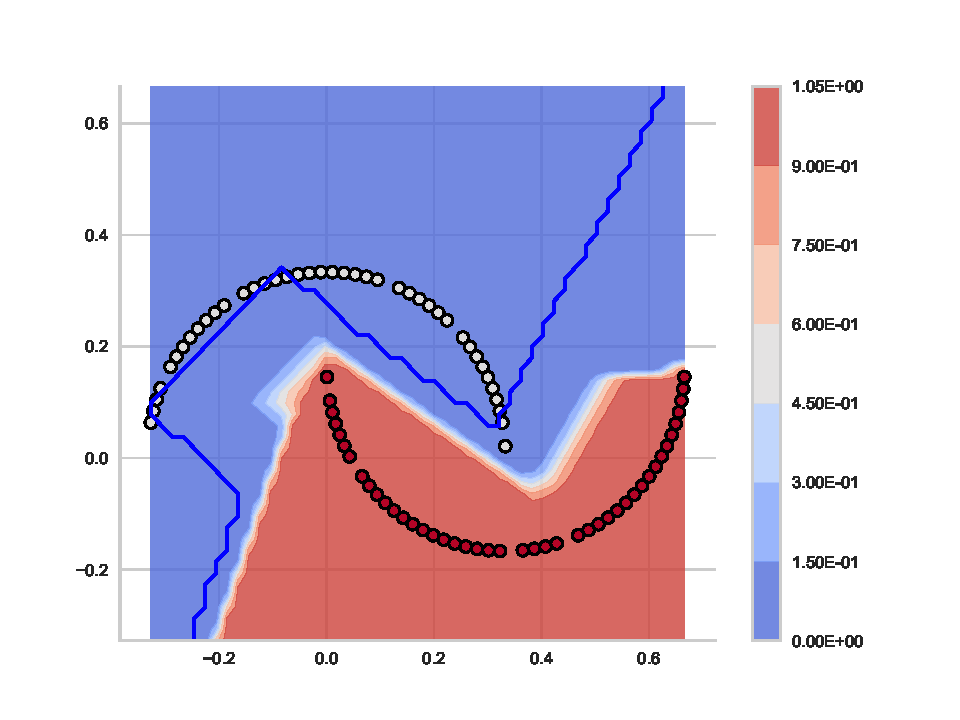
\includegraphics[width=\hsize]{img/toy/layerwise/output.pdf}}
    }
  }
    \caption{Data transformed across a 50x4 \SepLayer network. Although being a relaxation of \SepUnitPoint showing an intuitive solution with several affine and dead units. Indeed, they not only do not hinder the network but forward the solution 4th layer to the output.}
    \label{fig:moonsLayerwise}
\end{figure*}

\begin{figure*}
  \centering
    \begin{subfigure}[b]{0.3\textwidth}
        \includegraphics[width=\textwidth]{img/init/relu/conv2d_1-0.pdf}
        \caption{\ReLU input layer}
        \label{fig:reluInitInput}
    \end{subfigure}
    ~ %add desired spacing between images, e. g. ~, \quad, \qquad, \hfill etc. 
      %(or a blank line to force the subfigure onto a new line)
    \begin{subfigure}[b]{0.3\textwidth}
        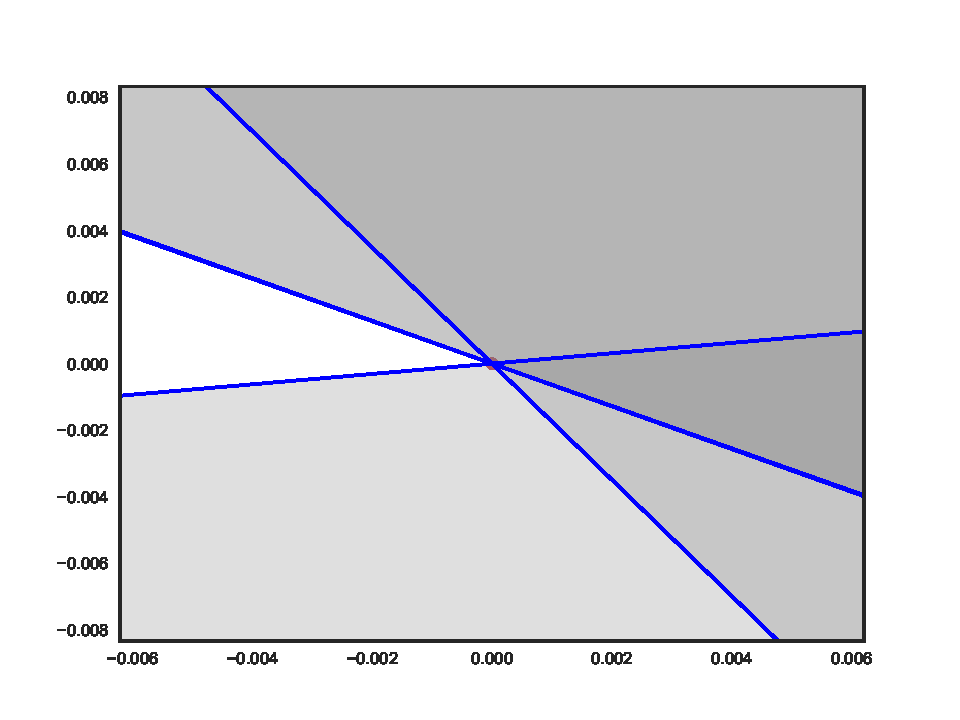
\includegraphics[width=\textwidth]{img/init/relu/conv2d_50-0.pdf}
        \caption{\ReLU 50th layer}
        \label{fig:reluInit501}
    \end{subfigure}
    ~ %add desired spacing between images, e. g. ~, \quad, \qquad, \hfill etc. 
    %(or a blank line to force the subfigure onto a new line)
    \begin{subfigure}[b]{0.3\textwidth}
        \includegraphics[width=\textwidth]{img/init/relu/conv2d_50-2.pdf}
        \caption{\ReLU 50th layer}
        \label{fig:reluInit502}
    \end{subfigure}
    \\
    \begin{subfigure}[b]{0.3\textwidth}
        \includegraphics[width=\textwidth]{img/init/relu-bn/conv2d_1-0.pdf}
        \caption{\ReLUBN input layer}
        \label{fig:reluBNInitInput}
    \end{subfigure}
    ~ %add desired spacing between images, e. g. ~, \quad, \qquad, \hfill etc. 
      %(or a blank line to force the subfigure onto a new line)
    \begin{subfigure}[b]{0.3\textwidth}
        \includegraphics[width=\textwidth]{img/init/relu-bn/conv2d_50-0.pdf}
        \caption{\ReLUBN 50th layer}
        \label{fig:reluBNInit501}
    \end{subfigure}
    ~ %add desired spacing between images, e. g. ~, \quad, \qquad, \hfill etc. 
    %(or a blank line to force the subfigure onto a new line)
    \begin{subfigure}[b]{0.3\textwidth}
        \includegraphics[width=\textwidth]{img/init/relu-bn/conv2d_50-2.pdf}
        \caption{\ReLUBN 50th layer}
        \label{fig:reluBNInit502}
    \end{subfigure}
    \\
    \begin{subfigure}[b]{0.3\textwidth}
        \includegraphics[width=\textwidth]{img/init/layerwise/conv2d_1-0.pdf}
        \caption{\SepLayer input layer}
        \label{fig:layerwiseInitInput}
    \end{subfigure}
    ~ %add desired spacing between images, e. g. ~, \quad, \qquad, \hfill etc. 
      %(or a blank line to force the subfigure onto a new line)
    \begin{subfigure}[b]{0.3\textwidth}
        \includegraphics[width=\textwidth]{img/init/layerwise/conv2d_50-0.pdf}
        \caption{\SepLayer 50th layer}
        \label{fig:layerwiseInit501}
    \end{subfigure}
    ~ %add desired spacing between images, e. g. ~, \quad, \qquad, \hfill etc. 
    %(or a blank line to force the subfigure onto a new line)
    \begin{subfigure}[b]{0.3\textwidth}
        \includegraphics[width=\textwidth]{img/init/layerwise/conv2d_50-2.pdf}
        \caption{\SepLayer 50th layer}
        \label{fig:layerwiseInit502}
    \end{subfigure}
    \\
    \begin{subfigure}[b]{0.3\textwidth}
        \includegraphics[width=\textwidth]{img/init/unitpointwise/conv2d_1-0.pdf}
        \caption{\SepUnitPoint Input}
        \label{fig:unitpointInitInput}
    \end{subfigure}
    ~ %add desired spacing between images, e. g. ~, \quad, \qquad, \hfill etc. 
      %(or a blank line to force the subfigure onto a new line)
    \begin{subfigure}[b]{0.3\textwidth}
        \includegraphics[width=\textwidth]{img/init/unitpointwise/conv2d_50-0.pdf}
        \caption{\SepUnitPoint 50th layer}
        \label{fig:unitpointInit501}
    \end{subfigure}
    ~ %add desired spacing between images, e. g. ~, \quad, \qquad, \hfill etc. 
    %(or a blank line to force the subfigure onto a new line)
    \begin{subfigure}[b]{0.3\textwidth}
        \includegraphics[width=\textwidth]{img/init/unitpointwise/conv2d_50-2.pdf}
        \caption{\SepUnitPoint 50th layer}
        \label{fig:unitpointInit502}
    \end{subfigure}
    
  \caption{Data transformed across a 50x4 network with no main loss (cross-entropy) with constraints \SepLayer and \SepUnitPoint, versus \ReLU and \ReLUBN. Notice how effectively \ReLU and \ReLUBN collapse the dataset into few points whereas \SepLayer and \SepUnitPoint force the network to learn representations that preserve geometrical structure useful for back-propagation.} 
  \label{fig:init} 
\end{figure*}



\begin{figure*}[h]
   
    \begin{subfigure}[c]{1\textwidth}
        \includegraphics[width=1\textwidth]{img/convergence/peaks_acc.pdf}
        \caption{Evolution of accuracy during training.}
        \label{fig:accuracy_convergence}
    \end{subfigure}
    \\
    
    \begin{subfigure}[c]{1\textwidth}
    \centering
        \includegraphics[width=1\textwidth]{img/convergence/peaks_loss.pdf}
        \caption{Evolution of cross-entropy and constraint loss during training.}
        \label{fig:loss_convergence}
    \end{subfigure}
    \\
   
\begin{subfigure}[b]{0.09\textwidth}
    \includegraphics[clip, trim=2.35cm 1.75cm 4.5cm 0cm,width=\textwidth]{img/convergence/0.pdf}
    \caption{0}
    \label{fig:convergence_0}
\end{subfigure}
%
        \end{figure*}
        \begin{figure*}[h]\ContinuedFloat
        
\begin{subfigure}[b]{0.09\textwidth}
    \includegraphics[clip, trim=2.35cm 1.75cm 4.5cm 0cm,width=\textwidth]{img/convergence/100.pdf}
    \caption{100}
    \label{fig:convergence_100}
\end{subfigure}
%
\begin{subfigure}[b]{0.09\textwidth}
    \includegraphics[clip, trim=2.35cm 1.75cm 4.5cm 0cm,width=\textwidth]{img/convergence/200.pdf}
    \caption{200}
    \label{fig:convergence_200}
\end{subfigure}
%
\begin{subfigure}[b]{0.09\textwidth}
    \includegraphics[clip, trim=2.35cm 1.75cm 4.5cm 0cm,width=\textwidth]{img/convergence/246.pdf}
    \caption{246}
    \label{fig:convergence_246}
\end{subfigure}
%
\begin{subfigure}[b]{0.09\textwidth}
    \includegraphics[clip, trim=2.35cm 1.75cm 4.5cm 0cm,width=\textwidth]{img/convergence/250.pdf}
    \caption{250}
    \label{fig:convergence_250}
\end{subfigure}
%
\begin{subfigure}[b]{0.09\textwidth}
    \includegraphics[clip, trim=2.35cm 1.75cm 4.5cm 0cm,width=\textwidth]{img/convergence/253.pdf}
    \caption{253}
    \label{fig:convergence_253}
\end{subfigure}
%
\begin{subfigure}[b]{0.09\textwidth}
    \includegraphics[clip, trim=2.35cm 1.75cm 4.5cm 0cm,width=\textwidth]{img/convergence/255.pdf}
    \caption{255}
    \label{fig:convergence_255}
\end{subfigure}
%
\begin{subfigure}[b]{0.09\textwidth}
    \includegraphics[clip, trim=2.35cm 1.75cm 4.5cm 0cm,width=\textwidth]{img/convergence/256.pdf}
    \caption{256}
    \label{fig:convergence_256}
\end{subfigure}
%
\begin{subfigure}[b]{0.09\textwidth}
    \includegraphics[clip, trim=2.35cm 1.75cm 4.5cm 0cm,width=\textwidth]{img/convergence/260.pdf}
    \caption{260}
    \label{fig:convergence_260}
\end{subfigure}
%
\begin{subfigure}[b]{0.09\textwidth}
    \includegraphics[clip, trim=2.35cm 1.75cm 4.5cm 0cm,width=\textwidth]{img/convergence/268.pdf}
    \caption{268}
    \label{fig:convergence_268}
\end{subfigure}
%
\begin{subfigure}[b]{0.09\textwidth}
    \includegraphics[clip, trim=2.35cm 1.75cm 4.5cm 0cm,width=\textwidth]{img/convergence/269.pdf}
    \caption{269}
    \label{fig:convergence_269}
\end{subfigure}
%
\begin{subfigure}[b]{0.09\textwidth}
    \includegraphics[clip, trim=2.35cm 1.75cm 4.5cm 0cm,width=\textwidth]{img/convergence/271.pdf}
    \caption{271}
    \label{fig:convergence_271}
\end{subfigure}
%
\begin{subfigure}[b]{0.09\textwidth}
    \includegraphics[clip, trim=2.35cm 1.75cm 4.5cm 0cm,width=\textwidth]{img/convergence/279.pdf}
    \caption{279}
    \label{fig:convergence_279}
\end{subfigure}
%
\begin{subfigure}[b]{0.09\textwidth}
    \includegraphics[clip, trim=2.35cm 1.75cm 4.5cm 0cm,width=\textwidth]{img/convergence/300.pdf}
    \caption{300}
    \label{fig:convergence_300}
\end{subfigure}
%
\begin{subfigure}[b]{0.09\textwidth}
    \includegraphics[clip, trim=2.35cm 1.75cm 4.5cm 0cm,width=\textwidth]{img/convergence/307.pdf}
    \caption{307}
    \label{fig:convergence_307}
\end{subfigure}
%
\begin{subfigure}[b]{0.09\textwidth}
    \includegraphics[clip, trim=2.35cm 1.75cm 4.5cm 0cm,width=\textwidth]{img/convergence/312.pdf}
    \caption{312}
    \label{fig:convergence_312}
\end{subfigure}
%
\begin{subfigure}[b]{0.09\textwidth}
    \includegraphics[clip, trim=2.35cm 1.75cm 4.5cm 0cm,width=\textwidth]{img/convergence/318.pdf}
    \caption{318}
    \label{fig:convergence_318}
\end{subfigure}
%
\begin{subfigure}[b]{0.09\textwidth}
    \includegraphics[clip, trim=2.35cm 1.75cm 4.5cm 0cm,width=\textwidth]{img/convergence/353.pdf}
    \caption{353}
    \label{fig:convergence_353}
\end{subfigure}
%
\begin{subfigure}[b]{0.09\textwidth}
    \includegraphics[clip, trim=2.35cm 1.75cm 4.5cm 0cm,width=\textwidth]{img/convergence/354.pdf}
    \caption{354}
    \label{fig:convergence_354}
\end{subfigure}
%
\begin{subfigure}[b]{0.09\textwidth}
    \includegraphics[clip, trim=2.35cm 1.75cm 4.5cm 0cm,width=\textwidth]{img/convergence/356.pdf}
    \caption{356}
    \label{fig:convergence_356}
\end{subfigure}
%
\begin{subfigure}[b]{0.09\textwidth}
    \includegraphics[clip, trim=2.35cm 1.75cm 4.5cm 0cm,width=\textwidth]{img/convergence/359.pdf}
    \caption{359}
    \label{fig:convergence_359}
\end{subfigure}
%
\begin{subfigure}[b]{0.09\textwidth}
    \includegraphics[clip, trim=2.35cm 1.75cm 4.5cm 0cm,width=\textwidth]{img/convergence/361.pdf}
    \caption{361}
    \label{fig:convergence_361}
\end{subfigure}
%
\begin{subfigure}[b]{0.09\textwidth}
    \includegraphics[clip, trim=2.35cm 1.75cm 4.5cm 0cm,width=\textwidth]{img/convergence/362.pdf}
    \caption{362}
    \label{fig:convergence_362}
\end{subfigure}
%
\begin{subfigure}[b]{0.09\textwidth}
    \includegraphics[clip, trim=2.35cm 1.75cm 4.5cm 0cm,width=\textwidth]{img/convergence/376.pdf}
    \caption{376}
    \label{fig:convergence_376}
\end{subfigure}
%
\begin{subfigure}[b]{0.09\textwidth}
    \includegraphics[clip, trim=2.35cm 1.75cm 4.5cm 0cm,width=\textwidth]{img/convergence/392.pdf}
    \caption{392}
    \label{fig:convergence_392}
\end{subfigure}
%
\begin{subfigure}[b]{0.09\textwidth}
    \includegraphics[clip, trim=2.35cm 1.75cm 4.5cm 0cm,width=\textwidth]{img/convergence/393.pdf}
    \caption{393}
    \label{fig:convergence_393}
\end{subfigure}
%
\begin{subfigure}[b]{0.09\textwidth}
    \includegraphics[clip, trim=2.35cm 1.75cm 4.5cm 0cm,width=\textwidth]{img/convergence/394.pdf}
    \caption{394}
    \label{fig:convergence_394}
\end{subfigure}
%
\begin{subfigure}[b]{0.09\textwidth}
    \includegraphics[clip, trim=2.35cm 1.75cm 4.5cm 0cm,width=\textwidth]{img/convergence/397.pdf}
    \caption{397}
    \label{fig:convergence_397}
\end{subfigure}
%
\begin{subfigure}[b]{0.09\textwidth}
    \includegraphics[clip, trim=2.35cm 1.75cm 4.5cm 0cm,width=\textwidth]{img/convergence/400.pdf}
    \caption{400}
    \label{fig:convergence_400}
\end{subfigure}
%
\begin{subfigure}[b]{0.09\textwidth}
    \includegraphics[clip, trim=2.35cm 1.75cm 4.5cm 0cm,width=\textwidth]{img/convergence/402.pdf}
    \caption{402}
    \label{fig:convergence_402}
\end{subfigure}
%
\begin{subfigure}[b]{0.09\textwidth}
    \includegraphics[clip, trim=2.35cm 1.75cm 4.5cm 0cm,width=\textwidth]{img/convergence/404.pdf}
    \caption{404}
    \label{fig:convergence_404}
\end{subfigure}
%
\begin{subfigure}[b]{0.09\textwidth}
    \includegraphics[clip, trim=2.35cm 1.75cm 4.5cm 0cm,width=\textwidth]{img/convergence/408.pdf}
    \caption{408}
    \label{fig:convergence_408}
\end{subfigure}
%
\begin{subfigure}[b]{0.09\textwidth}
    \includegraphics[clip, trim=2.35cm 1.75cm 4.5cm 0cm,width=\textwidth]{img/convergence/410.pdf}
    \caption{410}
    \label{fig:convergence_410}
\end{subfigure}
%
\begin{subfigure}[b]{0.09\textwidth}
    \includegraphics[clip, trim=2.35cm 1.75cm 4.5cm 0cm,width=\textwidth]{img/convergence/419.pdf}
    \caption{419}
    \label{fig:convergence_419}
\end{subfigure}
%
\begin{subfigure}[b]{0.09\textwidth}
    \includegraphics[clip, trim=2.35cm 1.75cm 4.5cm 0cm,width=\textwidth]{img/convergence/500.pdf}
    \caption{500}
    \label{fig:convergence_500}
\end{subfigure}
%
\begin{subfigure}[b]{0.09\textwidth}
    \includegraphics[clip, trim=2.35cm 1.75cm 4.5cm 0cm,width=\textwidth]{img/convergence/700.pdf}
    \caption{700}
    \label{fig:convergence_700}
\end{subfigure}
%
\begin{subfigure}[b]{0.09\textwidth}
    \includegraphics[clip, trim=2.35cm 1.75cm 4.5cm 0cm,width=\textwidth]{img/convergence/794.pdf}
    \caption{794}
    \label{fig:convergence_794}
\end{subfigure}
%
\begin{subfigure}[b]{0.09\textwidth}
    \includegraphics[clip, trim=2.35cm 1.75cm 4.5cm 0cm,width=\textwidth]{img/convergence/801.pdf}
    \caption{801}
    \label{fig:convergence_801}
\end{subfigure}
%
\begin{subfigure}[b]{0.09\textwidth}
    \includegraphics[clip, trim=2.35cm 1.75cm 4.5cm 0cm,width=\textwidth]{img/convergence/804.pdf}
    \caption{804}
    \label{fig:convergence_804}
\end{subfigure}
%
\begin{subfigure}[b]{0.09\textwidth}
    \includegraphics[clip, trim=2.35cm 1.75cm 4.5cm 0cm,width=\textwidth]{img/convergence/822.pdf}
    \caption{822}
    \label{fig:convergence_822}
\end{subfigure}
%
\begin{subfigure}[b]{0.09\textwidth}
    \includegraphics[clip, trim=2.35cm 1.75cm 4.5cm 0cm,width=\textwidth]{img/convergence/833.pdf}
    \caption{833}
    \label{fig:convergence_833}
\end{subfigure}
%
\begin{subfigure}[b]{0.09\textwidth}
    \includegraphics[clip, trim=2.35cm 1.75cm 4.5cm 0cm,width=\textwidth]{img/convergence/869.pdf}
    \caption{869}
    \label{fig:convergence_869}
\end{subfigure}
%
\begin{subfigure}[b]{0.09\textwidth}
    \includegraphics[clip, trim=2.35cm 1.75cm 4.5cm 0cm,width=\textwidth]{img/convergence/874.pdf}
    \caption{874}
    \label{fig:convergence_874}
\end{subfigure}
%
\begin{subfigure}[b]{0.09\textwidth}
    \includegraphics[clip, trim=2.35cm 1.75cm 4.5cm 0cm,width=\textwidth]{img/convergence/875.pdf}
    \caption{875}
    \label{fig:convergence_875}
\end{subfigure}
%
\begin{subfigure}[b]{0.09\textwidth}
    \includegraphics[clip, trim=2.35cm 1.75cm 4.5cm 0cm,width=\textwidth]{img/convergence/880.pdf}
    \caption{880}
    \label{fig:convergence_880}
\end{subfigure}
%
\begin{subfigure}[b]{0.09\textwidth}
    \includegraphics[clip, trim=2.35cm 1.75cm 4.5cm 0cm,width=\textwidth]{img/convergence/881.pdf}
    \caption{881}
    \label{fig:convergence_881}
\end{subfigure}
%
\begin{subfigure}[b]{0.09\textwidth}
    \includegraphics[clip, trim=2.35cm 1.75cm 4.5cm 0cm,width=\textwidth]{img/convergence/885.pdf}
    \caption{885}
    \label{fig:convergence_885}
\end{subfigure}
%
\begin{subfigure}[b]{0.09\textwidth}
    \includegraphics[clip, trim=2.35cm 1.75cm 4.5cm 0cm,width=\textwidth]{img/convergence/886.pdf}
    \caption{886}
    \label{fig:convergence_886}
\end{subfigure}
%
\begin{subfigure}[b]{0.09\textwidth}
    \includegraphics[clip, trim=2.35cm 1.75cm 4.5cm 0cm,width=\textwidth]{img/convergence/888.pdf}
    \caption{888}
    \label{fig:convergence_888}
\end{subfigure}
%
\begin{subfigure}[b]{0.09\textwidth}
    \includegraphics[clip, trim=2.35cm 1.75cm 4.5cm 0cm,width=\textwidth]{img/convergence/889.pdf}
    \caption{889}
    \label{fig:convergence_889}
\end{subfigure}
%
\begin{subfigure}[b]{0.09\textwidth}
    \includegraphics[clip, trim=2.35cm 1.75cm 4.5cm 0cm,width=\textwidth]{img/convergence/891.pdf}
    \caption{891}
    \label{fig:convergence_891}
\end{subfigure}
%
\begin{subfigure}[b]{0.09\textwidth}
    \includegraphics[clip, trim=2.35cm 1.75cm 4.5cm 0cm,width=\textwidth]{img/convergence/892.pdf}
    \caption{892}
    \label{fig:convergence_892}
\end{subfigure}
%
\begin{subfigure}[b]{0.09\textwidth}
    \includegraphics[clip, trim=2.35cm 1.75cm 4.5cm 0cm,width=\textwidth]{img/convergence/893.pdf}
    \caption{893}
    \label{fig:convergence_893}
\end{subfigure}
%
\begin{subfigure}[b]{0.09\textwidth}
    \includegraphics[clip, trim=2.35cm 1.75cm 4.5cm 0cm,width=\textwidth]{img/convergence/895.pdf}
    \caption{895}
    \label{fig:convergence_895}
\end{subfigure}
%
\begin{subfigure}[b]{0.09\textwidth}
    \includegraphics[clip, trim=2.35cm 1.75cm 4.5cm 0cm,width=\textwidth]{img/convergence/898.pdf}
    \caption{898}
    \label{fig:convergence_898}
\end{subfigure}
%
        \end{figure*}
        \begin{figure*}[h]\ContinuedFloat
        
\begin{subfigure}[b]{0.09\textwidth}
    \includegraphics[clip, trim=2.35cm 1.75cm 4.5cm 0cm,width=\textwidth]{img/convergence/900.pdf}
    \caption{900}
    \label{fig:convergence_900}
\end{subfigure}
%
\begin{subfigure}[b]{0.09\textwidth}
    \includegraphics[clip, trim=2.35cm 1.75cm 4.5cm 0cm,width=\textwidth]{img/convergence/904.pdf}
    \caption{904}
    \label{fig:convergence_904}
\end{subfigure}
%
\begin{subfigure}[b]{0.09\textwidth}
    \includegraphics[clip, trim=2.35cm 1.75cm 4.5cm 0cm,width=\textwidth]{img/convergence/905.pdf}
    \caption{905}
    \label{fig:convergence_905}
\end{subfigure}
%
\begin{subfigure}[b]{0.09\textwidth}
    \includegraphics[clip, trim=2.35cm 1.75cm 4.5cm 0cm,width=\textwidth]{img/convergence/908.pdf}
    \caption{908}
    \label{fig:convergence_908}
\end{subfigure}
%
\begin{subfigure}[b]{0.09\textwidth}
    \includegraphics[clip, trim=2.35cm 1.75cm 4.5cm 0cm,width=\textwidth]{img/convergence/966.pdf}
    \caption{966}
    \label{fig:convergence_966}
\end{subfigure}
%
\begin{subfigure}[b]{0.09\textwidth}
    \includegraphics[clip, trim=2.35cm 1.75cm 4.5cm 0cm,width=\textwidth]{img/convergence/998.pdf}
    \caption{998}
    \label{fig:convergence_998}
\end{subfigure}
%
\begin{subfigure}[b]{0.09\textwidth}
    \includegraphics[clip, trim=2.35cm 1.75cm 4.5cm 0cm,width=\textwidth]{img/convergence/1017.pdf}
    \caption{1017}
    \label{fig:convergence_1017}
\end{subfigure}
%
\begin{subfigure}[b]{0.09\textwidth}
    \includegraphics[clip, trim=2.35cm 1.75cm 4.5cm 0cm,width=\textwidth]{img/convergence/1100.pdf}
    \caption{1100}
    \label{fig:convergence_1100}
\end{subfigure}
%
\begin{subfigure}[b]{0.09\textwidth}
    \includegraphics[clip, trim=2.35cm 1.75cm 4.5cm 0cm,width=\textwidth]{img/convergence/1124.pdf}
    \caption{1124}
    \label{fig:convergence_1124}
\end{subfigure}
%
\begin{subfigure}[b]{0.09\textwidth}
    \includegraphics[clip, trim=2.35cm 1.75cm 4.5cm 0cm,width=\textwidth]{img/convergence/1130.pdf}
    \caption{1130}
    \label{fig:convergence_1130}
\end{subfigure}
%
\begin{subfigure}[b]{0.09\textwidth}
    \includegraphics[clip, trim=2.35cm 1.75cm 4.5cm 0cm,width=\textwidth]{img/convergence/1134.pdf}
    \caption{1134}
    \label{fig:convergence_1134}
\end{subfigure}
%
\begin{subfigure}[b]{0.09\textwidth}
    \includegraphics[clip, trim=2.35cm 1.75cm 4.5cm 0cm,width=\textwidth]{img/convergence/1135.pdf}
    \caption{1135}
    \label{fig:convergence_1135}
\end{subfigure}
%
\begin{subfigure}[b]{0.09\textwidth}
    \includegraphics[clip, trim=2.35cm 1.75cm 4.5cm 0cm,width=\textwidth]{img/convergence/1147.pdf}
    \caption{1147}
    \label{fig:convergence_1147}
\end{subfigure}
%
\begin{subfigure}[b]{0.09\textwidth}
    \includegraphics[clip, trim=2.35cm 1.75cm 4.5cm 0cm,width=\textwidth]{img/convergence/1161.pdf}
    \caption{1161}
    \label{fig:convergence_1161}
\end{subfigure}
%
\begin{subfigure}[b]{0.09\textwidth}
    \includegraphics[clip, trim=2.35cm 1.75cm 4.5cm 0cm,width=\textwidth]{img/convergence/1195.pdf}
    \caption{1195}
    \label{fig:convergence_1195}
\end{subfigure}
%
\begin{subfigure}[b]{0.09\textwidth}
    \includegraphics[clip, trim=2.35cm 1.75cm 4.5cm 0cm,width=\textwidth]{img/convergence/5000.pdf}
    \caption{5000}
    \label{fig:convergence_5000}
\end{subfigure}
%
\begin{subfigure}[b]{0.09\textwidth}
    \includegraphics[clip, trim=2.35cm 1.75cm 4.5cm 0cm,width=\textwidth]{img/convergence/5100.pdf}
    \caption{5100}
    \label{fig:convergence_5100}
\end{subfigure}
%
\begin{subfigure}[b]{0.09\textwidth}
    \includegraphics[clip, trim=2.35cm 1.75cm 4.5cm 0cm,width=\textwidth]{img/convergence/5200.pdf}
    \caption{5200}
    \label{fig:convergence_5200}
\end{subfigure}
%
\begin{subfigure}[b]{0.09\textwidth}
    \includegraphics[clip, trim=2.35cm 1.75cm 4.5cm 0cm,width=\textwidth]{img/convergence/6100.pdf}
    \caption{6100}
    \label{fig:convergence_6100}
\end{subfigure}
%
\begin{subfigure}[b]{0.09\textwidth}
    \includegraphics[clip, trim=2.35cm 1.75cm 4.5cm 0cm,width=\textwidth]{img/convergence/6200.pdf}
    \caption{6200}
    \label{fig:convergence_6200}
\end{subfigure}
%
\begin{subfigure}[b]{0.09\textwidth}
    \includegraphics[clip, trim=2.35cm 1.75cm 4.5cm 0cm,width=\textwidth]{img/convergence/6205.pdf}
    \caption{6205}
    \label{fig:convergence_6205}
\end{subfigure}
%
\begin{subfigure}[b]{0.09\textwidth}
    \includegraphics[clip, trim=2.35cm 1.75cm 4.5cm 0cm,width=\textwidth]{img/convergence/6206.pdf}
    \caption{6206}
    \label{fig:convergence_6206}
\end{subfigure}
%
\begin{subfigure}[b]{0.09\textwidth}
    \includegraphics[clip, trim=2.35cm 1.75cm 4.5cm 0cm,width=\textwidth]{img/convergence/6208.pdf}
    \caption{6208}
    \label{fig:convergence_6208}
\end{subfigure}
%
\begin{subfigure}[b]{0.09\textwidth}
    \includegraphics[clip, trim=2.35cm 1.75cm 4.5cm 0cm,width=\textwidth]{img/convergence/6219.pdf}
    \caption{6219}
    \label{fig:convergence_6219}
\end{subfigure}
%
\begin{subfigure}[b]{0.09\textwidth}
    \includegraphics[clip, trim=2.35cm 1.75cm 4.5cm 0cm,width=\textwidth]{img/convergence/6223.pdf}
    \caption{6223}
    \label{fig:convergence_6223}
\end{subfigure}
%
\begin{subfigure}[b]{0.09\textwidth}
    \includegraphics[clip, trim=2.35cm 1.75cm 4.5cm 0cm,width=\textwidth]{img/convergence/6224.pdf}
    \caption{6224}
    \label{fig:convergence_6224}
\end{subfigure}
%
\begin{subfigure}[b]{0.09\textwidth}
    \includegraphics[clip, trim=2.35cm 1.75cm 4.5cm 0cm,width=\textwidth]{img/convergence/6226.pdf}
    \caption{6226}
    \label{fig:convergence_6226}
\end{subfigure}
%
\begin{subfigure}[b]{0.09\textwidth}
    \includegraphics[clip, trim=2.35cm 1.75cm 4.5cm 0cm,width=\textwidth]{img/convergence/6227.pdf}
    \caption{6227}
    \label{fig:convergence_6227}
\end{subfigure}
%
\begin{subfigure}[b]{0.09\textwidth}
    \includegraphics[clip, trim=2.35cm 1.75cm 4.5cm 0cm,width=\textwidth]{img/convergence/6228.pdf}
    \caption{6228}
    \label{fig:convergence_6228}
\end{subfigure}
%
\begin{subfigure}[b]{0.09\textwidth}
    \includegraphics[clip, trim=2.35cm 1.75cm 4.5cm 0cm,width=\textwidth]{img/convergence/6229.pdf}
    \caption{6229}
    \label{fig:convergence_6229}
\end{subfigure}
%
\begin{subfigure}[b]{0.09\textwidth}
    \includegraphics[clip, trim=2.35cm 1.75cm 4.5cm 0cm,width=\textwidth]{img/convergence/6242.pdf}
    \caption{6242}
    \label{fig:convergence_6242}
\end{subfigure}
%
\begin{subfigure}[b]{0.09\textwidth}
    \includegraphics[clip, trim=2.35cm 1.75cm 4.5cm 0cm,width=\textwidth]{img/convergence/6300.pdf}
    \caption{6300}
    \label{fig:convergence_6300}
\end{subfigure}
%
\begin{subfigure}[b]{0.09\textwidth}
    \includegraphics[clip, trim=2.35cm 1.75cm 4.5cm 0cm,width=\textwidth]{img/convergence/6400.pdf}
    \caption{6400}
    \label{fig:convergence_6400}
\end{subfigure}
%
\begin{subfigure}[b]{0.09\textwidth}
    \includegraphics[clip, trim=2.35cm 1.75cm 4.5cm 0cm,width=\textwidth]{img/convergence/6500.pdf}
    \caption{6500}
    \label{fig:convergence_6500}
\end{subfigure}
%
\begin{subfigure}[b]{0.09\textwidth}
    \includegraphics[clip, trim=2.35cm 1.75cm 4.5cm 0cm,width=\textwidth]{img/convergence/6600.pdf}
    \caption{6600}
    \label{fig:convergence_6600}
\end{subfigure}
%
\begin{subfigure}[b]{0.09\textwidth}
    \includegraphics[clip, trim=2.35cm 1.75cm 4.5cm 0cm,width=\textwidth]{img/convergence/6700.pdf}
    \caption{6700}
    \label{fig:convergence_6700}
\end{subfigure}
%
\begin{subfigure}[b]{0.09\textwidth}
    \includegraphics[clip, trim=2.35cm 1.75cm 4.5cm 0cm,width=\textwidth]{img/convergence/6738.pdf}
    \caption{6738}
    \label{fig:convergence_6738}
\end{subfigure}
%
\begin{subfigure}[b]{0.09\textwidth}
    \includegraphics[clip, trim=2.35cm 1.75cm 4.5cm 0cm,width=\textwidth]{img/convergence/6742.pdf}
    \caption{6742}
    \label{fig:convergence_6742}
\end{subfigure}
%
\begin{subfigure}[b]{0.09\textwidth}
    \includegraphics[clip, trim=2.35cm 1.75cm 4.5cm 0cm,width=\textwidth]{img/convergence/6745.pdf}
    \caption{6745}
    \label{fig:convergence_6745}
\end{subfigure}
%
\begin{subfigure}[b]{0.09\textwidth}
    \includegraphics[clip, trim=2.35cm 1.75cm 4.5cm 0cm,width=\textwidth]{img/convergence/6746.pdf}
    \caption{6746}
    \label{fig:convergence_6746}
\end{subfigure}
%
\begin{subfigure}[b]{0.09\textwidth}
    \includegraphics[clip, trim=2.35cm 1.75cm 4.5cm 0cm,width=\textwidth]{img/convergence/6748.pdf}
    \caption{6748}
    \label{fig:convergence_6748}
\end{subfigure}
%
\begin{subfigure}[b]{0.09\textwidth}
    \includegraphics[clip, trim=2.35cm 1.75cm 4.5cm 0cm,width=\textwidth]{img/convergence/6749.pdf}
    \caption{6749}
    \label{fig:convergence_6749}
\end{subfigure}
%
\begin{subfigure}[b]{0.09\textwidth}
    \includegraphics[clip, trim=2.35cm 1.75cm 4.5cm 0cm,width=\textwidth]{img/convergence/6774.pdf}
    \caption{6774}
    \label{fig:convergence_6774}
\end{subfigure}
%
\begin{subfigure}[b]{0.09\textwidth}
    \includegraphics[clip, trim=2.35cm 1.75cm 4.5cm 0cm,width=\textwidth]{img/convergence/6777.pdf}
    \caption{6777}
    \label{fig:convergence_6777}
\end{subfigure}
%
\begin{subfigure}[b]{0.09\textwidth}
    \includegraphics[clip, trim=2.35cm 1.75cm 4.5cm 0cm,width=\textwidth]{img/convergence/6780.pdf}
    \caption{6780}
    \label{fig:convergence_6780}
\end{subfigure}
%
\begin{subfigure}[b]{0.09\textwidth}
    \includegraphics[clip, trim=2.35cm 1.75cm 4.5cm 0cm,width=\textwidth]{img/convergence/6781.pdf}
    \caption{6781}
    \label{fig:convergence_6781}
\end{subfigure}
%
\begin{subfigure}[b]{0.09\textwidth}
    \includegraphics[clip, trim=2.35cm 1.75cm 4.5cm 0cm,width=\textwidth]{img/convergence/6782.pdf}
    \caption{6782}
    \label{fig:convergence_6782}
\end{subfigure}
%
\begin{subfigure}[b]{0.09\textwidth}
    \includegraphics[clip, trim=2.35cm 1.75cm 4.5cm 0cm,width=\textwidth]{img/convergence/6794.pdf}
    \caption{6794}
    \label{fig:convergence_6794}
\end{subfigure}
%
\begin{subfigure}[b]{0.09\textwidth}
    \includegraphics[clip, trim=2.35cm 1.75cm 4.5cm 0cm,width=\textwidth]{img/convergence/6795.pdf}
    \caption{6795}
    \label{fig:convergence_6795}
\end{subfigure}
%
\begin{subfigure}[b]{0.09\textwidth}
    \includegraphics[clip, trim=2.35cm 1.75cm 4.5cm 0cm,width=\textwidth]{img/convergence/6796.pdf}
    \caption{6796}
    \label{fig:convergence_6796}
\end{subfigure}
%
\begin{subfigure}[b]{0.09\textwidth}
    \includegraphics[clip, trim=2.35cm 1.75cm 4.5cm 0cm,width=\textwidth]{img/convergence/6797.pdf}
    \caption{6797}
    \label{fig:convergence_6797}
\end{subfigure}
%
\begin{subfigure}[b]{0.09\textwidth}
    \includegraphics[clip, trim=2.35cm 1.75cm 4.5cm 0cm,width=\textwidth]{img/convergence/6798.pdf}
    \caption{6798}
    \label{fig:convergence_6798}
\end{subfigure}
%
\begin{subfigure}[b]{0.09\textwidth}
    \includegraphics[clip, trim=2.35cm 1.75cm 4.5cm 0cm,width=\textwidth]{img/convergence/6799.pdf}
    \caption{6799}
    \label{fig:convergence_6799}
\end{subfigure}
%
\begin{subfigure}[b]{0.09\textwidth}
    \includegraphics[clip, trim=2.35cm 1.75cm 4.5cm 0cm,width=\textwidth]{img/convergence/6800.pdf}
    \caption{6800}
    \label{fig:convergence_6800}
\end{subfigure}
%
        \end{figure*}
        \begin{figure*}[h]\ContinuedFloat
        
\begin{subfigure}[b]{0.09\textwidth}
    \includegraphics[clip, trim=2.35cm 1.75cm 4.5cm 0cm,width=\textwidth]{img/convergence/6811.pdf}
    \caption{6811}
    \label{fig:convergence_6811}
\end{subfigure}
%
\begin{subfigure}[b]{0.09\textwidth}
    \includegraphics[clip, trim=2.35cm 1.75cm 4.5cm 0cm,width=\textwidth]{img/convergence/6812.pdf}
    \caption{6812}
    \label{fig:convergence_6812}
\end{subfigure}
%
\begin{subfigure}[b]{0.09\textwidth}
    \includegraphics[clip, trim=2.35cm 1.75cm 4.5cm 0cm,width=\textwidth]{img/convergence/6813.pdf}
    \caption{6813}
    \label{fig:convergence_6813}
\end{subfigure}
%
\begin{subfigure}[b]{0.09\textwidth}
    \includegraphics[clip, trim=2.35cm 1.75cm 4.5cm 0cm,width=\textwidth]{img/convergence/6814.pdf}
    \caption{6814}
    \label{fig:convergence_6814}
\end{subfigure}
%
\begin{subfigure}[b]{0.09\textwidth}
    \includegraphics[clip, trim=2.35cm 1.75cm 4.5cm 0cm,width=\textwidth]{img/convergence/6842.pdf}
    \caption{6842}
    \label{fig:convergence_6842}
\end{subfigure}
%
\begin{subfigure}[b]{0.09\textwidth}
    \includegraphics[clip, trim=2.35cm 1.75cm 4.5cm 0cm,width=\textwidth]{img/convergence/6843.pdf}
    \caption{6843}
    \label{fig:convergence_6843}
\end{subfigure}
%
\begin{subfigure}[b]{0.09\textwidth}
    \includegraphics[clip, trim=2.35cm 1.75cm 4.5cm 0cm,width=\textwidth]{img/convergence/6844.pdf}
    \caption{6844}
    \label{fig:convergence_6844}
\end{subfigure}
%
\begin{subfigure}[b]{0.09\textwidth}
    \includegraphics[clip, trim=2.35cm 1.75cm 4.5cm 0cm,width=\textwidth]{img/convergence/6845.pdf}
    \caption{6845}
    \label{fig:convergence_6845}
\end{subfigure}
%
\begin{subfigure}[b]{0.09\textwidth}
    \includegraphics[clip, trim=2.35cm 1.75cm 4.5cm 0cm,width=\textwidth]{img/convergence/6846.pdf}
    \caption{6846}
    \label{fig:convergence_6846}
\end{subfigure}
%
\begin{subfigure}[b]{0.09\textwidth}
    \includegraphics[clip, trim=2.35cm 1.75cm 4.5cm 0cm,width=\textwidth]{img/convergence/6847.pdf}
    \caption{6847}
    \label{fig:convergence_6847}
\end{subfigure}
%
\begin{subfigure}[b]{0.09\textwidth}
    \includegraphics[clip, trim=2.35cm 1.75cm 4.5cm 0cm,width=\textwidth]{img/convergence/6848.pdf}
    \caption{6848}
    \label{fig:convergence_6848}
\end{subfigure}
%
\begin{subfigure}[b]{0.09\textwidth}
    \includegraphics[clip, trim=2.35cm 1.75cm 4.5cm 0cm,width=\textwidth]{img/convergence/6853.pdf}
    \caption{6853}
    \label{fig:convergence_6853}
\end{subfigure}
%
\begin{subfigure}[b]{0.09\textwidth}
    \includegraphics[clip, trim=2.35cm 1.75cm 4.5cm 0cm,width=\textwidth]{img/convergence/6857.pdf}
    \caption{6857}
    \label{fig:convergence_6857}
\end{subfigure}
%
\begin{subfigure}[b]{0.09\textwidth}
    \includegraphics[clip, trim=2.35cm 1.75cm 4.5cm 0cm,width=\textwidth]{img/convergence/6877.pdf}
    \caption{6877}
    \label{fig:convergence_6877}
\end{subfigure}
%
\begin{subfigure}[b]{0.09\textwidth}
    \includegraphics[clip, trim=2.35cm 1.75cm 4.5cm 0cm,width=\textwidth]{img/convergence/6900.pdf}
    \caption{6900}
    \label{fig:convergence_6900}
\end{subfigure}
%
\begin{subfigure}[b]{0.09\textwidth}
    \includegraphics[clip, trim=2.35cm 1.75cm 4.5cm 0cm,width=\textwidth]{img/convergence/7000.pdf}
    \caption{7000}
    \label{fig:convergence_7000}
\end{subfigure}
%
\begin{subfigure}[b]{0.09\textwidth}
    \includegraphics[clip, trim=2.35cm 1.75cm 4.5cm 0cm,width=\textwidth]{img/convergence/7019.pdf}
    \caption{7019}
    \label{fig:convergence_7019}
\end{subfigure}
%
\begin{subfigure}[b]{0.09\textwidth}
    \includegraphics[clip, trim=2.35cm 1.75cm 4.5cm 0cm,width=\textwidth]{img/convergence/7020.pdf}
    \caption{7020}
    \label{fig:convergence_7020}
\end{subfigure}
%
\begin{subfigure}[b]{0.09\textwidth}
    \includegraphics[clip, trim=2.35cm 1.75cm 4.5cm 0cm,width=\textwidth]{img/convergence/7025.pdf}
    \caption{7025}
    \label{fig:convergence_7025}
\end{subfigure}
%
\begin{subfigure}[b]{0.09\textwidth}
    \includegraphics[clip, trim=2.35cm 1.75cm 4.5cm 0cm,width=\textwidth]{img/convergence/7026.pdf}
    \caption{7026}
    \label{fig:convergence_7026}
\end{subfigure}
%
\begin{subfigure}[b]{0.09\textwidth}
    \includegraphics[clip, trim=2.35cm 1.75cm 4.5cm 0cm,width=\textwidth]{img/convergence/7027.pdf}
    \caption{7027}
    \label{fig:convergence_7027}
\end{subfigure}
%
\begin{subfigure}[b]{0.09\textwidth}
    \includegraphics[clip, trim=2.35cm 1.75cm 4.5cm 0cm,width=\textwidth]{img/convergence/7030.pdf}
    \caption{7030}
    \label{fig:convergence_7030}
\end{subfigure}
%
\begin{subfigure}[b]{0.09\textwidth}
    \includegraphics[clip, trim=2.35cm 1.75cm 4.5cm 0cm,width=\textwidth]{img/convergence/7036.pdf}
    \caption{7036}
    \label{fig:convergence_7036}
\end{subfigure}
%
\begin{subfigure}[b]{0.09\textwidth}
    \includegraphics[clip, trim=2.35cm 1.75cm 4.5cm 0cm,width=\textwidth]{img/convergence/7048.pdf}
    \caption{7048}
    \label{fig:convergence_7048}
\end{subfigure}
%
\begin{subfigure}[b]{0.09\textwidth}
    \includegraphics[clip, trim=2.35cm 1.75cm 4.5cm 0cm,width=\textwidth]{img/convergence/7054.pdf}
    \caption{7054}
    \label{fig:convergence_7054}
\end{subfigure}
%
\begin{subfigure}[b]{0.09\textwidth}
    \includegraphics[clip, trim=2.35cm 1.75cm 4.5cm 0cm,width=\textwidth]{img/convergence/7055.pdf}
    \caption{7055}
    \label{fig:convergence_7055}
\end{subfigure}
%
\begin{subfigure}[b]{0.09\textwidth}
    \includegraphics[clip, trim=2.35cm 1.75cm 4.5cm 0cm,width=\textwidth]{img/convergence/7056.pdf}
    \caption{7056}
    \label{fig:convergence_7056}
\end{subfigure}
%
\begin{subfigure}[b]{0.09\textwidth}
    \includegraphics[clip, trim=2.35cm 1.75cm 4.5cm 0cm,width=\textwidth]{img/convergence/7057.pdf}
    \caption{7057}
    \label{fig:convergence_7057}
\end{subfigure}
%
\begin{subfigure}[b]{0.09\textwidth}
    \includegraphics[clip, trim=2.35cm 1.75cm 4.5cm 0cm,width=\textwidth]{img/convergence/7058.pdf}
    \caption{7058}
    \label{fig:convergence_7058}
\end{subfigure}
%
\begin{subfigure}[b]{0.09\textwidth}
    \includegraphics[clip, trim=2.35cm 1.75cm 4.5cm 0cm,width=\textwidth]{img/convergence/7063.pdf}
    \caption{7063}
    \label{fig:convergence_7063}
\end{subfigure}
%
\begin{subfigure}[b]{0.09\textwidth}
    \includegraphics[clip, trim=2.35cm 1.75cm 4.5cm 0cm,width=\textwidth]{img/convergence/7066.pdf}
    \caption{7066}
    \label{fig:convergence_7066}
\end{subfigure}
%
\begin{subfigure}[b]{0.09\textwidth}
    \includegraphics[clip, trim=2.35cm 1.75cm 4.5cm 0cm,width=\textwidth]{img/convergence/7067.pdf}
    \caption{7067}
    \label{fig:convergence_7067}
\end{subfigure}
%
\begin{subfigure}[b]{0.09\textwidth}
    \includegraphics[clip, trim=2.35cm 1.75cm 4.5cm 0cm,width=\textwidth]{img/convergence/7069.pdf}
    \caption{7069}
    \label{fig:convergence_7069}
\end{subfigure}
%
\begin{subfigure}[b]{0.09\textwidth}
    \includegraphics[clip, trim=2.35cm 1.75cm 4.5cm 0cm,width=\textwidth]{img/convergence/7070.pdf}
    \caption{7070}
    \label{fig:convergence_7070}
\end{subfigure}
%
\begin{subfigure}[b]{0.09\textwidth}
    \includegraphics[clip, trim=2.35cm 1.75cm 4.5cm 0cm,width=\textwidth]{img/convergence/7071.pdf}
    \caption{7071}
    \label{fig:convergence_7071}
\end{subfigure}
%
\begin{subfigure}[b]{0.09\textwidth}
    \includegraphics[clip, trim=2.35cm 1.75cm 4.5cm 0cm,width=\textwidth]{img/convergence/7072.pdf}
    \caption{7072}
    \label{fig:convergence_7072}
\end{subfigure}
%
\begin{subfigure}[b]{0.09\textwidth}
    \includegraphics[clip, trim=2.35cm 1.75cm 4.5cm 0cm,width=\textwidth]{img/convergence/7073.pdf}
    \caption{7073}
    \label{fig:convergence_7073}
\end{subfigure}
%
\begin{subfigure}[b]{0.09\textwidth}
    \includegraphics[clip, trim=2.35cm 1.75cm 4.5cm 0cm,width=\textwidth]{img/convergence/7074.pdf}
    \caption{7074}
    \label{fig:convergence_7074}
\end{subfigure}
%
\begin{subfigure}[b]{0.09\textwidth}
    \includegraphics[clip, trim=2.35cm 1.75cm 4.5cm 0cm,width=\textwidth]{img/convergence/7075.pdf}
    \caption{7075}
    \label{fig:convergence_7075}
\end{subfigure}
%
\begin{subfigure}[b]{0.09\textwidth}
    \includegraphics[clip, trim=2.35cm 1.75cm 4.5cm 0cm,width=\textwidth]{img/convergence/7077.pdf}
    \caption{7077}
    \label{fig:convergence_7077}
\end{subfigure}
%
\begin{subfigure}[b]{0.09\textwidth}
    \includegraphics[clip, trim=2.35cm 1.75cm 4.5cm 0cm,width=\textwidth]{img/convergence/7079.pdf}
    \caption{7079}
    \label{fig:convergence_7079}
\end{subfigure}
%
\begin{subfigure}[b]{0.09\textwidth}
    \includegraphics[clip, trim=2.35cm 1.75cm 4.5cm 0cm,width=\textwidth]{img/convergence/7080.pdf}
    \caption{7080}
    \label{fig:convergence_7080}
\end{subfigure}
%
\begin{subfigure}[b]{0.09\textwidth}
    \includegraphics[clip, trim=2.35cm 1.75cm 4.5cm 0cm,width=\textwidth]{img/convergence/7081.pdf}
    \caption{7081}
    \label{fig:convergence_7081}
\end{subfigure}
%
\begin{subfigure}[b]{0.09\textwidth}
    \includegraphics[clip, trim=2.35cm 1.75cm 4.5cm 0cm,width=\textwidth]{img/convergence/7082.pdf}
    \caption{7082}
    \label{fig:convergence_7082}
\end{subfigure}
%
\begin{subfigure}[b]{0.09\textwidth}
    \includegraphics[clip, trim=2.35cm 1.75cm 4.5cm 0cm,width=\textwidth]{img/convergence/7083.pdf}
    \caption{7083}
    \label{fig:convergence_7083}
\end{subfigure}
%
\begin{subfigure}[b]{0.09\textwidth}
    \includegraphics[clip, trim=2.35cm 1.75cm 4.5cm 0cm,width=\textwidth]{img/convergence/7084.pdf}
    \caption{7084}
    \label{fig:convergence_7084}
\end{subfigure}
%
\begin{subfigure}[b]{0.09\textwidth}
    \includegraphics[clip, trim=2.35cm 1.75cm 4.5cm 0cm,width=\textwidth]{img/convergence/7085.pdf}
    \caption{7085}
    \label{fig:convergence_7085}
\end{subfigure}
%
\begin{subfigure}[b]{0.09\textwidth}
    \includegraphics[clip, trim=2.35cm 1.75cm 4.5cm 0cm,width=\textwidth]{img/convergence/7086.pdf}
    \caption{7086}
    \label{fig:convergence_7086}
\end{subfigure}
%
\begin{subfigure}[b]{0.09\textwidth}
    \includegraphics[clip, trim=2.35cm 1.75cm 4.5cm 0cm,width=\textwidth]{img/convergence/7088.pdf}
    \caption{7088}
    \label{fig:convergence_7088}
\end{subfigure}
%
\begin{subfigure}[b]{0.09\textwidth}
    \includegraphics[clip, trim=2.35cm 1.75cm 4.5cm 0cm,width=\textwidth]{img/convergence/7099.pdf}
    \caption{7099}
    \label{fig:convergence_7099}
\end{subfigure}
%
\begin{subfigure}[b]{0.09\textwidth}
    \includegraphics[clip, trim=2.35cm 1.75cm 4.5cm 0cm,width=\textwidth]{img/convergence/7104.pdf}
    \caption{7104}
    \label{fig:convergence_7104}
\end{subfigure}
%
\begin{subfigure}[b]{0.09\textwidth}
    \includegraphics[clip, trim=2.35cm 1.75cm 4.5cm 0cm,width=\textwidth]{img/convergence/7114.pdf}
    \caption{7114}
    \label{fig:convergence_7114}
\end{subfigure}
%
\begin{subfigure}[b]{0.09\textwidth}
    \includegraphics[clip, trim=2.35cm 1.75cm 4.5cm 0cm,width=\textwidth]{img/convergence/7115.pdf}
    \caption{7115}
    \label{fig:convergence_7115}
\end{subfigure}
%
\begin{subfigure}[b]{0.09\textwidth}
    \includegraphics[clip, trim=2.35cm 1.75cm 4.5cm 0cm,width=\textwidth]{img/convergence/7127.pdf}
    \caption{7127}
    \label{fig:convergence_7127}
\end{subfigure}
%
        \end{figure*}
        \begin{figure*}[h]\ContinuedFloat
        
\begin{subfigure}[b]{0.09\textwidth}
    \includegraphics[clip, trim=2.35cm 1.75cm 4.5cm 0cm,width=\textwidth]{img/convergence/7500.pdf}
    \caption{7500}
    \label{fig:convergence_7500}
\end{subfigure}
%
\begin{subfigure}[b]{0.09\textwidth}
    \includegraphics[clip, trim=2.35cm 1.75cm 4.5cm 0cm,width=\textwidth]{img/convergence/8128.pdf}
    \caption{8128}
    \label{fig:convergence_8128}
\end{subfigure}
%
\begin{subfigure}[b]{0.09\textwidth}
    \includegraphics[clip, trim=2.35cm 1.75cm 4.5cm 0cm,width=\textwidth]{img/convergence/8129.pdf}
    \caption{8129}
    \label{fig:convergence_8129}
\end{subfigure}
%
\begin{subfigure}[b]{0.09\textwidth}
    \includegraphics[clip, trim=2.35cm 1.75cm 4.5cm 0cm,width=\textwidth]{img/convergence/8130.pdf}
    \caption{8130}
    \label{fig:convergence_8130}
\end{subfigure}
%
\begin{subfigure}[b]{0.09\textwidth}
    \includegraphics[clip, trim=2.35cm 1.75cm 4.5cm 0cm,width=\textwidth]{img/convergence/8131.pdf}
    \caption{8131}
    \label{fig:convergence_8131}
\end{subfigure}
%
\begin{subfigure}[b]{0.09\textwidth}
    \includegraphics[clip, trim=2.35cm 1.75cm 4.5cm 0cm,width=\textwidth]{img/convergence/8132.pdf}
    \caption{8132}
    \label{fig:convergence_8132}
\end{subfigure}
%
\begin{subfigure}[b]{0.09\textwidth}
    \includegraphics[clip, trim=2.35cm 1.75cm 4.5cm 0cm,width=\textwidth]{img/convergence/8133.pdf}
    \caption{8133}
    \label{fig:convergence_8133}
\end{subfigure}
%
\begin{subfigure}[b]{0.09\textwidth}
    \includegraphics[clip, trim=2.35cm 1.75cm 4.5cm 0cm,width=\textwidth]{img/convergence/8135.pdf}
    \caption{8135}
    \label{fig:convergence_8135}
\end{subfigure}
%
\begin{subfigure}[b]{0.09\textwidth}
    \includegraphics[clip, trim=2.35cm 1.75cm 4.5cm 0cm,width=\textwidth]{img/convergence/8137.pdf}
    \caption{8137}
    \label{fig:convergence_8137}
\end{subfigure}
%
\begin{subfigure}[b]{0.09\textwidth}
    \includegraphics[clip, trim=2.35cm 1.75cm 4.5cm 0cm,width=\textwidth]{img/convergence/8138.pdf}
    \caption{8138}
    \label{fig:convergence_8138}
\end{subfigure}
%
\begin{subfigure}[b]{0.09\textwidth}
    \includegraphics[clip, trim=2.35cm 1.75cm 4.5cm 0cm,width=\textwidth]{img/convergence/8139.pdf}
    \caption{8139}
    \label{fig:convergence_8139}
\end{subfigure}
%
\begin{subfigure}[b]{0.09\textwidth}
    \includegraphics[clip, trim=2.35cm 1.75cm 4.5cm 0cm,width=\textwidth]{img/convergence/8140.pdf}
    \caption{8140}
    \label{fig:convergence_8140}
\end{subfigure}
%
\begin{subfigure}[b]{0.09\textwidth}
    \includegraphics[clip, trim=2.35cm 1.75cm 4.5cm 0cm,width=\textwidth]{img/convergence/8141.pdf}
    \caption{8141}
    \label{fig:convergence_8141}
\end{subfigure}
%
\begin{subfigure}[b]{0.09\textwidth}
    \includegraphics[clip, trim=2.35cm 1.75cm 4.5cm 0cm,width=\textwidth]{img/convergence/8142.pdf}
    \caption{8142}
    \label{fig:convergence_8142}
\end{subfigure}
%
\begin{subfigure}[b]{0.09\textwidth}
    \includegraphics[clip, trim=2.35cm 1.75cm 4.5cm 0cm,width=\textwidth]{img/convergence/8144.pdf}
    \caption{8144}
    \label{fig:convergence_8144}
\end{subfigure}
%
\begin{subfigure}[b]{0.09\textwidth}
    \includegraphics[clip, trim=2.35cm 1.75cm 4.5cm 0cm,width=\textwidth]{img/convergence/8145.pdf}
    \caption{8145}
    \label{fig:convergence_8145}
\end{subfigure}
%
\begin{subfigure}[b]{0.09\textwidth}
    \includegraphics[clip, trim=2.35cm 1.75cm 4.5cm 0cm,width=\textwidth]{img/convergence/8146.pdf}
    \caption{8146}
    \label{fig:convergence_8146}
\end{subfigure}
%
\begin{subfigure}[b]{0.09\textwidth}
    \includegraphics[clip, trim=2.35cm 1.75cm 4.5cm 0cm,width=\textwidth]{img/convergence/8147.pdf}
    \caption{8147}
    \label{fig:convergence_8147}
\end{subfigure}
%
\begin{subfigure}[b]{0.09\textwidth}
    \includegraphics[clip, trim=2.35cm 1.75cm 4.5cm 0cm,width=\textwidth]{img/convergence/8148.pdf}
    \caption{8148}
    \label{fig:convergence_8148}
\end{subfigure}
%
\begin{subfigure}[b]{0.09\textwidth}
    \includegraphics[clip, trim=2.35cm 1.75cm 4.5cm 0cm,width=\textwidth]{img/convergence/8150.pdf}
    \caption{8150}
    \label{fig:convergence_8150}
\end{subfigure}
%
\begin{subfigure}[b]{0.09\textwidth}
    \includegraphics[clip, trim=2.35cm 1.75cm 4.5cm 0cm,width=\textwidth]{img/convergence/8151.pdf}
    \caption{8151}
    \label{fig:convergence_8151}
\end{subfigure}
%
\begin{subfigure}[b]{0.09\textwidth}
    \includegraphics[clip, trim=2.35cm 1.75cm 4.5cm 0cm,width=\textwidth]{img/convergence/8154.pdf}
    \caption{8154}
    \label{fig:convergence_8154}
\end{subfigure}
%
\begin{subfigure}[b]{0.09\textwidth}
    \includegraphics[clip, trim=2.35cm 1.75cm 4.5cm 0cm,width=\textwidth]{img/convergence/8159.pdf}
    \caption{8159}
    \label{fig:convergence_8159}
\end{subfigure}
%
\begin{subfigure}[b]{0.09\textwidth}
    \includegraphics[clip, trim=2.35cm 1.75cm 4.5cm 0cm,width=\textwidth]{img/convergence/8163.pdf}
    \caption{8163}
    \label{fig:convergence_8163}
\end{subfigure}
%
\begin{subfigure}[b]{0.09\textwidth}
    \includegraphics[clip, trim=2.35cm 1.75cm 4.5cm 0cm,width=\textwidth]{img/convergence/8171.pdf}
    \caption{8171}
    \label{fig:convergence_8171}
\end{subfigure}
%
\begin{subfigure}[b]{0.09\textwidth}
    \includegraphics[clip, trim=2.35cm 1.75cm 4.5cm 0cm,width=\textwidth]{img/convergence/8173.pdf}
    \caption{8173}
    \label{fig:convergence_8173}
\end{subfigure}
%
\begin{subfigure}[b]{0.09\textwidth}
    \includegraphics[clip, trim=2.35cm 1.75cm 4.5cm 0cm,width=\textwidth]{img/convergence/8176.pdf}
    \caption{8176}
    \label{fig:convergence_8176}
\end{subfigure}
%
\begin{subfigure}[b]{0.09\textwidth}
    \includegraphics[clip, trim=2.35cm 1.75cm 4.5cm 0cm,width=\textwidth]{img/convergence/8185.pdf}
    \caption{8185}
    \label{fig:convergence_8185}
\end{subfigure}
%
\begin{subfigure}[b]{0.09\textwidth}
    \includegraphics[clip, trim=2.35cm 1.75cm 4.5cm 0cm,width=\textwidth]{img/convergence/8188.pdf}
    \caption{8188}
    \label{fig:convergence_8188}
\end{subfigure}
%
\begin{subfigure}[b]{0.09\textwidth}
    \includegraphics[clip, trim=2.35cm 1.75cm 4.5cm 0cm,width=\textwidth]{img/convergence/8193.pdf}
    \caption{8193}
    \label{fig:convergence_8193}
\end{subfigure}
%
\begin{subfigure}[b]{0.09\textwidth}
    \includegraphics[clip, trim=2.35cm 1.75cm 4.5cm 0cm,width=\textwidth]{img/convergence/8215.pdf}
    \caption{8215}
    \label{fig:convergence_8215}
\end{subfigure}
%
\begin{subfigure}[b]{0.09\textwidth}
    \includegraphics[clip, trim=2.35cm 1.75cm 4.5cm 0cm,width=\textwidth]{img/convergence/8246.pdf}
    \caption{8246}
    \label{fig:convergence_8246}
\end{subfigure}
%
\begin{subfigure}[b]{0.09\textwidth}
    \includegraphics[clip, trim=2.35cm 1.75cm 4.5cm 0cm,width=\textwidth]{img/convergence/8249.pdf}
    \caption{8249}
    \label{fig:convergence_8249}
\end{subfigure}
%
\begin{subfigure}[b]{0.09\textwidth}
    \includegraphics[clip, trim=2.35cm 1.75cm 4.5cm 0cm,width=\textwidth]{img/convergence/8250.pdf}
    \caption{8250}
    \label{fig:convergence_8250}
\end{subfigure}
%
\begin{subfigure}[b]{0.09\textwidth}
    \includegraphics[clip, trim=2.35cm 1.75cm 4.5cm 0cm,width=\textwidth]{img/convergence/8269.pdf}
    \caption{8269}
    \label{fig:convergence_8269}
\end{subfigure}
%
\begin{subfigure}[b]{0.09\textwidth}
    \includegraphics[clip, trim=2.35cm 1.75cm 4.5cm 0cm,width=\textwidth]{img/convergence/8278.pdf}
    \caption{8278}
    \label{fig:convergence_8278}
\end{subfigure}
%
\begin{subfigure}[b]{0.09\textwidth}
    \includegraphics[clip, trim=2.35cm 1.75cm 4.5cm 0cm,width=\textwidth]{img/convergence/8291.pdf}
    \caption{8291}
    \label{fig:convergence_8291}
\end{subfigure}
%
\begin{subfigure}[b]{0.09\textwidth}
    \includegraphics[clip, trim=2.35cm 1.75cm 4.5cm 0cm,width=\textwidth]{img/convergence/8300.pdf}
    \caption{8300}
    \label{fig:convergence_8300}
\end{subfigure}
%
\begin{subfigure}[b]{0.09\textwidth}
    \includegraphics[clip, trim=2.35cm 1.75cm 4.5cm 0cm,width=\textwidth]{img/convergence/8305.pdf}
    \caption{8305}
    \label{fig:convergence_8305}
\end{subfigure}
%
\begin{subfigure}[b]{0.09\textwidth}
    \includegraphics[clip, trim=2.35cm 1.75cm 4.5cm 0cm,width=\textwidth]{img/convergence/8308.pdf}
    \caption{8308}
    \label{fig:convergence_8308}
\end{subfigure}
%
\begin{subfigure}[b]{0.09\textwidth}
    \includegraphics[clip, trim=2.35cm 1.75cm 4.5cm 0cm,width=\textwidth]{img/convergence/8334.pdf}
    \caption{8334}
    \label{fig:convergence_8334}
\end{subfigure}
%
\begin{subfigure}[b]{0.09\textwidth}
    \includegraphics[clip, trim=2.35cm 1.75cm 4.5cm 0cm,width=\textwidth]{img/convergence/8336.pdf}
    \caption{8336}
    \label{fig:convergence_8336}
\end{subfigure}
%
\begin{subfigure}[b]{0.09\textwidth}
    \includegraphics[clip, trim=2.35cm 1.75cm 4.5cm 0cm,width=\textwidth]{img/convergence/8344.pdf}
    \caption{8344}
    \label{fig:convergence_8344}
\end{subfigure}
%
\begin{subfigure}[b]{0.09\textwidth}
    \includegraphics[clip, trim=2.35cm 1.75cm 4.5cm 0cm,width=\textwidth]{img/convergence/8345.pdf}
    \caption{8345}
    \label{fig:convergence_8345}
\end{subfigure}
%
\begin{subfigure}[b]{0.09\textwidth}
    \includegraphics[clip, trim=2.35cm 1.75cm 4.5cm 0cm,width=\textwidth]{img/convergence/8346.pdf}
    \caption{8346}
    \label{fig:convergence_8346}
\end{subfigure}
%
\begin{subfigure}[b]{0.09\textwidth}
    \includegraphics[clip, trim=2.35cm 1.75cm 4.5cm 0cm,width=\textwidth]{img/convergence/8353.pdf}
    \caption{8353}
    \label{fig:convergence_8353}
\end{subfigure}
%
\begin{subfigure}[b]{0.09\textwidth}
    \includegraphics[clip, trim=2.35cm 1.75cm 4.5cm 0cm,width=\textwidth]{img/convergence/8354.pdf}
    \caption{8354}
    \label{fig:convergence_8354}
\end{subfigure}
%
\begin{subfigure}[b]{0.09\textwidth}
    \includegraphics[clip, trim=2.35cm 1.75cm 4.5cm 0cm,width=\textwidth]{img/convergence/8355.pdf}
    \caption{8355}
    \label{fig:convergence_8355}
\end{subfigure}
%
\begin{subfigure}[b]{0.09\textwidth}
    \includegraphics[clip, trim=2.35cm 1.75cm 4.5cm 0cm,width=\textwidth]{img/convergence/8356.pdf}
    \caption{8356}
    \label{fig:convergence_8356}
\end{subfigure}
%
\begin{subfigure}[b]{0.09\textwidth}
    \includegraphics[clip, trim=2.35cm 1.75cm 4.5cm 0cm,width=\textwidth]{img/convergence/8358.pdf}
    \caption{8358}
    \label{fig:convergence_8358}
\end{subfigure}
%
\begin{subfigure}[b]{0.09\textwidth}
    \includegraphics[clip, trim=2.35cm 1.75cm 4.5cm 0cm,width=\textwidth]{img/convergence/8361.pdf}
    \caption{8361}
    \label{fig:convergence_8361}
\end{subfigure}
%
\begin{subfigure}[b]{0.09\textwidth}
    \includegraphics[clip, trim=2.35cm 1.75cm 4.5cm 0cm,width=\textwidth]{img/convergence/8363.pdf}
    \caption{8363}
    \label{fig:convergence_8363}
\end{subfigure}
%
\begin{subfigure}[b]{0.09\textwidth}
    \includegraphics[clip, trim=2.35cm 1.75cm 4.5cm 0cm,width=\textwidth]{img/convergence/8364.pdf}
    \caption{8364}
    \label{fig:convergence_8364}
\end{subfigure}
%
\begin{subfigure}[b]{0.09\textwidth}
    \includegraphics[clip, trim=2.35cm 1.75cm 4.5cm 0cm,width=\textwidth]{img/convergence/8365.pdf}
    \caption{8365}
    \label{fig:convergence_8365}
\end{subfigure}
%
        \end{figure*}
        \begin{figure*}[h]\ContinuedFloat
        
\begin{subfigure}[b]{0.09\textwidth}
    \includegraphics[clip, trim=2.35cm 1.75cm 4.5cm 0cm,width=\textwidth]{img/convergence/8382.pdf}
    \caption{8382}
    \label{fig:convergence_8382}
\end{subfigure}
%
\begin{subfigure}[b]{0.09\textwidth}
    \includegraphics[clip, trim=2.35cm 1.75cm 4.5cm 0cm,width=\textwidth]{img/convergence/8400.pdf}
    \caption{8400}
    \label{fig:convergence_8400}
\end{subfigure}
%
\begin{subfigure}[b]{0.09\textwidth}
    \includegraphics[clip, trim=2.35cm 1.75cm 4.5cm 0cm,width=\textwidth]{img/convergence/8500.pdf}
    \caption{8500}
    \label{fig:convergence_8500}
\end{subfigure}
%
\begin{subfigure}[b]{0.09\textwidth}
    \includegraphics[clip, trim=2.35cm 1.75cm 4.5cm 0cm,width=\textwidth]{img/convergence/8512.pdf}
    \caption{8512}
    \label{fig:convergence_8512}
\end{subfigure}
%
\begin{subfigure}[b]{0.09\textwidth}
    \includegraphics[clip, trim=2.35cm 1.75cm 4.5cm 0cm,width=\textwidth]{img/convergence/8513.pdf}
    \caption{8513}
    \label{fig:convergence_8513}
\end{subfigure}
%
\begin{subfigure}[b]{0.09\textwidth}
    \includegraphics[clip, trim=2.35cm 1.75cm 4.5cm 0cm,width=\textwidth]{img/convergence/8514.pdf}
    \caption{8514}
    \label{fig:convergence_8514}
\end{subfigure}
%
\begin{subfigure}[b]{0.09\textwidth}
    \includegraphics[clip, trim=2.35cm 1.75cm 4.5cm 0cm,width=\textwidth]{img/convergence/8515.pdf}
    \caption{8515}
    \label{fig:convergence_8515}
\end{subfigure}
%
\begin{subfigure}[b]{0.09\textwidth}
    \includegraphics[clip, trim=2.35cm 1.75cm 4.5cm 0cm,width=\textwidth]{img/convergence/8516.pdf}
    \caption{8516}
    \label{fig:convergence_8516}
\end{subfigure}
%
\begin{subfigure}[b]{0.09\textwidth}
    \includegraphics[clip, trim=2.35cm 1.75cm 4.5cm 0cm,width=\textwidth]{img/convergence/8517.pdf}
    \caption{8517}
    \label{fig:convergence_8517}
\end{subfigure}
%
\begin{subfigure}[b]{0.09\textwidth}
    \includegraphics[clip, trim=2.35cm 1.75cm 4.5cm 0cm,width=\textwidth]{img/convergence/8521.pdf}
    \caption{8521}
    \label{fig:convergence_8521}
\end{subfigure}
%
\begin{subfigure}[b]{0.09\textwidth}
    \includegraphics[clip, trim=2.35cm 1.75cm 4.5cm 0cm,width=\textwidth]{img/convergence/8522.pdf}
    \caption{8522}
    \label{fig:convergence_8522}
\end{subfigure}
%
\begin{subfigure}[b]{0.09\textwidth}
    \includegraphics[clip, trim=2.35cm 1.75cm 4.5cm 0cm,width=\textwidth]{img/convergence/8523.pdf}
    \caption{8523}
    \label{fig:convergence_8523}
\end{subfigure}
%
\begin{subfigure}[b]{0.09\textwidth}
    \includegraphics[clip, trim=2.35cm 1.75cm 4.5cm 0cm,width=\textwidth]{img/convergence/8526.pdf}
    \caption{8526}
    \label{fig:convergence_8526}
\end{subfigure}
%
\begin{subfigure}[b]{0.09\textwidth}
    \includegraphics[clip, trim=2.35cm 1.75cm 4.5cm 0cm,width=\textwidth]{img/convergence/8529.pdf}
    \caption{8529}
    \label{fig:convergence_8529}
\end{subfigure}
%
\begin{subfigure}[b]{0.09\textwidth}
    \includegraphics[clip, trim=2.35cm 1.75cm 4.5cm 0cm,width=\textwidth]{img/convergence/8534.pdf}
    \caption{8534}
    \label{fig:convergence_8534}
\end{subfigure}
%
\begin{subfigure}[b]{0.09\textwidth}
    \includegraphics[clip, trim=2.35cm 1.75cm 4.5cm 0cm,width=\textwidth]{img/convergence/8536.pdf}
    \caption{8536}
    \label{fig:convergence_8536}
\end{subfigure}
%
\begin{subfigure}[b]{0.09\textwidth}
    \includegraphics[clip, trim=2.35cm 1.75cm 4.5cm 0cm,width=\textwidth]{img/convergence/8540.pdf}
    \caption{8540}
    \label{fig:convergence_8540}
\end{subfigure}
%
\begin{subfigure}[b]{0.09\textwidth}
    \includegraphics[clip, trim=2.35cm 1.75cm 4.5cm 0cm,width=\textwidth]{img/convergence/8541.pdf}
    \caption{8541}
    \label{fig:convergence_8541}
\end{subfigure}
%
\begin{subfigure}[b]{0.09\textwidth}
    \includegraphics[clip, trim=2.35cm 1.75cm 4.5cm 0cm,width=\textwidth]{img/convergence/8542.pdf}
    \caption{8542}
    \label{fig:convergence_8542}
\end{subfigure}
%
\begin{subfigure}[b]{0.09\textwidth}
    \includegraphics[clip, trim=2.35cm 1.75cm 4.5cm 0cm,width=\textwidth]{img/convergence/8543.pdf}
    \caption{8543}
    \label{fig:convergence_8543}
\end{subfigure}
%
\begin{subfigure}[b]{0.09\textwidth}
    \includegraphics[clip, trim=2.35cm 1.75cm 4.5cm 0cm,width=\textwidth]{img/convergence/8544.pdf}
    \caption{8544}
    \label{fig:convergence_8544}
\end{subfigure}
%
\begin{subfigure}[b]{0.09\textwidth}
    \includegraphics[clip, trim=2.35cm 1.75cm 4.5cm 0cm,width=\textwidth]{img/convergence/8545.pdf}
    \caption{8545}
    \label{fig:convergence_8545}
\end{subfigure}
%
\begin{subfigure}[b]{0.09\textwidth}
    \includegraphics[clip, trim=2.35cm 1.75cm 4.5cm 0cm,width=\textwidth]{img/convergence/8546.pdf}
    \caption{8546}
    \label{fig:convergence_8546}
\end{subfigure}
%
\begin{subfigure}[b]{0.09\textwidth}
    \includegraphics[clip, trim=2.35cm 1.75cm 4.5cm 0cm,width=\textwidth]{img/convergence/8547.pdf}
    \caption{8547}
    \label{fig:convergence_8547}
\end{subfigure}
%
\begin{subfigure}[b]{0.09\textwidth}
    \includegraphics[clip, trim=2.35cm 1.75cm 4.5cm 0cm,width=\textwidth]{img/convergence/8548.pdf}
    \caption{8548}
    \label{fig:convergence_8548}
\end{subfigure}
%
\begin{subfigure}[b]{0.09\textwidth}
    \includegraphics[clip, trim=2.35cm 1.75cm 4.5cm 0cm,width=\textwidth]{img/convergence/8567.pdf}
    \caption{8567}
    \label{fig:convergence_8567}
\end{subfigure}
%
\begin{subfigure}[b]{0.09\textwidth}
    \includegraphics[clip, trim=2.35cm 1.75cm 4.5cm 0cm,width=\textwidth]{img/convergence/8573.pdf}
    \caption{8573}
    \label{fig:convergence_8573}
\end{subfigure}
%
\begin{subfigure}[b]{0.09\textwidth}
    \includegraphics[clip, trim=2.35cm 1.75cm 4.5cm 0cm,width=\textwidth]{img/convergence/8574.pdf}
    \caption{8574}
    \label{fig:convergence_8574}
\end{subfigure}
%
\begin{subfigure}[b]{0.09\textwidth}
    \includegraphics[clip, trim=2.35cm 1.75cm 4.5cm 0cm,width=\textwidth]{img/convergence/8575.pdf}
    \caption{8575}
    \label{fig:convergence_8575}
\end{subfigure}
%
\begin{subfigure}[b]{0.09\textwidth}
    \includegraphics[clip, trim=2.35cm 1.75cm 4.5cm 0cm,width=\textwidth]{img/convergence/8578.pdf}
    \caption{8578}
    \label{fig:convergence_8578}
\end{subfigure}
%
\begin{subfigure}[b]{0.09\textwidth}
    \includegraphics[clip, trim=2.35cm 1.75cm 4.5cm 0cm,width=\textwidth]{img/convergence/8588.pdf}
    \caption{8588}
    \label{fig:convergence_8588}
\end{subfigure}
%
\begin{subfigure}[b]{0.09\textwidth}
    \includegraphics[clip, trim=2.35cm 1.75cm 4.5cm 0cm,width=\textwidth]{img/convergence/8589.pdf}
    \caption{8589}
    \label{fig:convergence_8589}
\end{subfigure}
%
\begin{subfigure}[b]{0.09\textwidth}
    \includegraphics[clip, trim=2.35cm 1.75cm 4.5cm 0cm,width=\textwidth]{img/convergence/8654.pdf}
    \caption{8654}
    \label{fig:convergence_8654}
\end{subfigure}
%
\begin{subfigure}[b]{0.09\textwidth}
    \includegraphics[clip, trim=2.35cm 1.75cm 4.5cm 0cm,width=\textwidth]{img/convergence/8658.pdf}
    \caption{8658}
    \label{fig:convergence_8658}
\end{subfigure}
%
\begin{subfigure}[b]{0.09\textwidth}
    \includegraphics[clip, trim=2.35cm 1.75cm 4.5cm 0cm,width=\textwidth]{img/convergence/8661.pdf}
    \caption{8661}
    \label{fig:convergence_8661}
\end{subfigure}
%
\begin{subfigure}[b]{0.09\textwidth}
    \includegraphics[clip, trim=2.35cm 1.75cm 4.5cm 0cm,width=\textwidth]{img/convergence/8664.pdf}
    \caption{8664}
    \label{fig:convergence_8664}
\end{subfigure}
%
\begin{subfigure}[b]{0.09\textwidth}
    \includegraphics[clip, trim=2.35cm 1.75cm 4.5cm 0cm,width=\textwidth]{img/convergence/8800.pdf}
    \caption{8800}
    \label{fig:convergence_8800}
\end{subfigure}
%
\begin{subfigure}[b]{0.09\textwidth}
    \includegraphics[clip, trim=2.35cm 1.75cm 4.5cm 0cm,width=\textwidth]{img/convergence/9000.pdf}
    \caption{9000}
    \label{fig:convergence_9000}
\end{subfigure}
%
\begin{subfigure}[b]{0.09\textwidth}
    \includegraphics[clip, trim=2.35cm 1.75cm 4.5cm 0cm,width=\textwidth]{img/convergence/9048.pdf}
    \caption{9048}
    \label{fig:convergence_9048}
\end{subfigure}
%
\begin{subfigure}[b]{0.09\textwidth}
    \includegraphics[clip, trim=2.35cm 1.75cm 4.5cm 0cm,width=\textwidth]{img/convergence/9049.pdf}
    \caption{9049}
    \label{fig:convergence_9049}
\end{subfigure}
%
\begin{subfigure}[b]{0.09\textwidth}
    \includegraphics[clip, trim=2.35cm 1.75cm 4.5cm 0cm,width=\textwidth]{img/convergence/9052.pdf}
    \caption{9052}
    \label{fig:convergence_9052}
\end{subfigure}
%
\begin{subfigure}[b]{0.09\textwidth}
    \includegraphics[clip, trim=2.35cm 1.75cm 4.5cm 0cm,width=\textwidth]{img/convergence/9053.pdf}
    \caption{9053}
    \label{fig:convergence_9053}
\end{subfigure}
%
\begin{subfigure}[b]{0.09\textwidth}
    \includegraphics[clip, trim=2.35cm 1.75cm 4.5cm 0cm,width=\textwidth]{img/convergence/9055.pdf}
    \caption{9055}
    \label{fig:convergence_9055}
\end{subfigure}
%
\begin{subfigure}[b]{0.09\textwidth}
    \includegraphics[clip, trim=2.35cm 1.75cm 4.5cm 0cm,width=\textwidth]{img/convergence/9057.pdf}
    \caption{9057}
    \label{fig:convergence_9057}
\end{subfigure}
%
\begin{subfigure}[b]{0.09\textwidth}
    \includegraphics[clip, trim=2.35cm 1.75cm 4.5cm 0cm,width=\textwidth]{img/convergence/9072.pdf}
    \caption{9072}
    \label{fig:convergence_9072}
\end{subfigure}
%
\begin{subfigure}[b]{0.09\textwidth}
    \includegraphics[clip, trim=2.35cm 1.75cm 4.5cm 0cm,width=\textwidth]{img/convergence/9074.pdf}
    \caption{9074}
    \label{fig:convergence_9074}
\end{subfigure}
%
\begin{subfigure}[b]{0.09\textwidth}
    \includegraphics[clip, trim=2.35cm 1.75cm 4.5cm 0cm,width=\textwidth]{img/convergence/9075.pdf}
    \caption{9075}
    \label{fig:convergence_9075}
\end{subfigure}
%
\begin{subfigure}[b]{0.09\textwidth}
    \includegraphics[clip, trim=2.35cm 1.75cm 4.5cm 0cm,width=\textwidth]{img/convergence/9077.pdf}
    \caption{9077}
    \label{fig:convergence_9077}
\end{subfigure}
%
\begin{subfigure}[b]{0.09\textwidth}
    \includegraphics[clip, trim=2.35cm 1.75cm 4.5cm 0cm,width=\textwidth]{img/convergence/9079.pdf}
    \caption{9079}
    \label{fig:convergence_9079}
\end{subfigure}
%
\begin{subfigure}[b]{0.09\textwidth}
    \includegraphics[clip, trim=2.35cm 1.75cm 4.5cm 0cm,width=\textwidth]{img/convergence/9080.pdf}
    \caption{9080}
    \label{fig:convergence_9080}
\end{subfigure}
%
\begin{subfigure}[b]{0.09\textwidth}
    \includegraphics[clip, trim=2.35cm 1.75cm 4.5cm 0cm,width=\textwidth]{img/convergence/9081.pdf}
    \caption{9081}
    \label{fig:convergence_9081}
\end{subfigure}
%
\begin{subfigure}[b]{0.09\textwidth}
    \includegraphics[clip, trim=2.35cm 1.75cm 4.5cm 0cm,width=\textwidth]{img/convergence/9082.pdf}
    \caption{9082}
    \label{fig:convergence_9082}
\end{subfigure}
%
\begin{subfigure}[b]{0.09\textwidth}
    \includegraphics[clip, trim=2.35cm 1.75cm 4.5cm 0cm,width=\textwidth]{img/convergence/9083.pdf}
    \caption{9083}
    \label{fig:convergence_9083}
\end{subfigure}
%
\begin{subfigure}[b]{0.09\textwidth}
    \includegraphics[clip, trim=2.35cm 1.75cm 4.5cm 0cm,width=\textwidth]{img/convergence/9084.pdf}
    \caption{9084}
    \label{fig:convergence_9084}
\end{subfigure}
%
        \end{figure*}
        \begin{figure*}[h]\ContinuedFloat
        
\begin{subfigure}[b]{0.09\textwidth}
    \includegraphics[clip, trim=2.35cm 1.75cm 4.5cm 0cm,width=\textwidth]{img/convergence/9090.pdf}
    \caption{9090}
    \label{fig:convergence_9090}
\end{subfigure}
%
\begin{subfigure}[b]{0.09\textwidth}
    \includegraphics[clip, trim=2.35cm 1.75cm 4.5cm 0cm,width=\textwidth]{img/convergence/9091.pdf}
    \caption{9091}
    \label{fig:convergence_9091}
\end{subfigure}
%
\begin{subfigure}[b]{0.09\textwidth}
    \includegraphics[clip, trim=2.35cm 1.75cm 4.5cm 0cm,width=\textwidth]{img/convergence/9092.pdf}
    \caption{9092}
    \label{fig:convergence_9092}
\end{subfigure}
%
\begin{subfigure}[b]{0.09\textwidth}
    \includegraphics[clip, trim=2.35cm 1.75cm 4.5cm 0cm,width=\textwidth]{img/convergence/9093.pdf}
    \caption{9093}
    \label{fig:convergence_9093}
\end{subfigure}
%
\begin{subfigure}[b]{0.09\textwidth}
    \includegraphics[clip, trim=2.35cm 1.75cm 4.5cm 0cm,width=\textwidth]{img/convergence/9094.pdf}
    \caption{9094}
    \label{fig:convergence_9094}
\end{subfigure}
%
\begin{subfigure}[b]{0.09\textwidth}
    \includegraphics[clip, trim=2.35cm 1.75cm 4.5cm 0cm,width=\textwidth]{img/convergence/9095.pdf}
    \caption{9095}
    \label{fig:convergence_9095}
\end{subfigure}
%
\begin{subfigure}[b]{0.09\textwidth}
    \includegraphics[clip, trim=2.35cm 1.75cm 4.5cm 0cm,width=\textwidth]{img/convergence/9096.pdf}
    \caption{9096}
    \label{fig:convergence_9096}
\end{subfigure}
%
\begin{subfigure}[b]{0.09\textwidth}
    \includegraphics[clip, trim=2.35cm 1.75cm 4.5cm 0cm,width=\textwidth]{img/convergence/9097.pdf}
    \caption{9097}
    \label{fig:convergence_9097}
\end{subfigure}
%
\begin{subfigure}[b]{0.09\textwidth}
    \includegraphics[clip, trim=2.35cm 1.75cm 4.5cm 0cm,width=\textwidth]{img/convergence/9098.pdf}
    \caption{9098}
    \label{fig:convergence_9098}
\end{subfigure}
%
\begin{subfigure}[b]{0.09\textwidth}
    \includegraphics[clip, trim=2.35cm 1.75cm 4.5cm 0cm,width=\textwidth]{img/convergence/9100.pdf}
    \caption{9100}
    \label{fig:convergence_9100}
\end{subfigure}
%
\begin{subfigure}[b]{0.09\textwidth}
    \includegraphics[clip, trim=2.35cm 1.75cm 4.5cm 0cm,width=\textwidth]{img/convergence/9101.pdf}
    \caption{9101}
    \label{fig:convergence_9101}
\end{subfigure}
%
\begin{subfigure}[b]{0.09\textwidth}
    \includegraphics[clip, trim=2.35cm 1.75cm 4.5cm 0cm,width=\textwidth]{img/convergence/9102.pdf}
    \caption{9102}
    \label{fig:convergence_9102}
\end{subfigure}
%
\begin{subfigure}[b]{0.09\textwidth}
    \includegraphics[clip, trim=2.35cm 1.75cm 4.5cm 0cm,width=\textwidth]{img/convergence/9103.pdf}
    \caption{9103}
    \label{fig:convergence_9103}
\end{subfigure}
%
\begin{subfigure}[b]{0.09\textwidth}
    \includegraphics[clip, trim=2.35cm 1.75cm 4.5cm 0cm,width=\textwidth]{img/convergence/9104.pdf}
    \caption{9104}
    \label{fig:convergence_9104}
\end{subfigure}
%
\begin{subfigure}[b]{0.09\textwidth}
    \includegraphics[clip, trim=2.35cm 1.75cm 4.5cm 0cm,width=\textwidth]{img/convergence/9109.pdf}
    \caption{9109}
    \label{fig:convergence_9109}
\end{subfigure}
%
\begin{subfigure}[b]{0.09\textwidth}
    \includegraphics[clip, trim=2.35cm 1.75cm 4.5cm 0cm,width=\textwidth]{img/convergence/9111.pdf}
    \caption{9111}
    \label{fig:convergence_9111}
\end{subfigure}
%
\begin{subfigure}[b]{0.09\textwidth}
    \includegraphics[clip, trim=2.35cm 1.75cm 4.5cm 0cm,width=\textwidth]{img/convergence/9114.pdf}
    \caption{9114}
    \label{fig:convergence_9114}
\end{subfigure}
%
\begin{subfigure}[b]{0.09\textwidth}
    \includegraphics[clip, trim=2.35cm 1.75cm 4.5cm 0cm,width=\textwidth]{img/convergence/9115.pdf}
    \caption{9115}
    \label{fig:convergence_9115}
\end{subfigure}
%
\begin{subfigure}[b]{0.09\textwidth}
    \includegraphics[clip, trim=2.35cm 1.75cm 4.5cm 0cm,width=\textwidth]{img/convergence/9119.pdf}
    \caption{9119}
    \label{fig:convergence_9119}
\end{subfigure}
%
\begin{subfigure}[b]{0.09\textwidth}
    \includegraphics[clip, trim=2.35cm 1.75cm 4.5cm 0cm,width=\textwidth]{img/convergence/9120.pdf}
    \caption{9120}
    \label{fig:convergence_9120}
\end{subfigure}
%
\begin{subfigure}[b]{0.09\textwidth}
    \includegraphics[clip, trim=2.35cm 1.75cm 4.5cm 0cm,width=\textwidth]{img/convergence/9123.pdf}
    \caption{9123}
    \label{fig:convergence_9123}
\end{subfigure}
%
\begin{subfigure}[b]{0.09\textwidth}
    \includegraphics[clip, trim=2.35cm 1.75cm 4.5cm 0cm,width=\textwidth]{img/convergence/9125.pdf}
    \caption{9125}
    \label{fig:convergence_9125}
\end{subfigure}
%
\begin{subfigure}[b]{0.09\textwidth}
    \includegraphics[clip, trim=2.35cm 1.75cm 4.5cm 0cm,width=\textwidth]{img/convergence/9128.pdf}
    \caption{9128}
    \label{fig:convergence_9128}
\end{subfigure}
%
\begin{subfigure}[b]{0.09\textwidth}
    \includegraphics[clip, trim=2.35cm 1.75cm 4.5cm 0cm,width=\textwidth]{img/convergence/9129.pdf}
    \caption{9129}
    \label{fig:convergence_9129}
\end{subfigure}
%
\begin{subfigure}[b]{0.09\textwidth}
    \includegraphics[clip, trim=2.35cm 1.75cm 4.5cm 0cm,width=\textwidth]{img/convergence/9130.pdf}
    \caption{9130}
    \label{fig:convergence_9130}
\end{subfigure}
%
\begin{subfigure}[b]{0.09\textwidth}
    \includegraphics[clip, trim=2.35cm 1.75cm 4.5cm 0cm,width=\textwidth]{img/convergence/9133.pdf}
    \caption{9133}
    \label{fig:convergence_9133}
\end{subfigure}
%
\begin{subfigure}[b]{0.09\textwidth}
    \includegraphics[clip, trim=2.35cm 1.75cm 4.5cm 0cm,width=\textwidth]{img/convergence/9135.pdf}
    \caption{9135}
    \label{fig:convergence_9135}
\end{subfigure}
%
\begin{subfigure}[b]{0.09\textwidth}
    \includegraphics[clip, trim=2.35cm 1.75cm 4.5cm 0cm,width=\textwidth]{img/convergence/9136.pdf}
    \caption{9136}
    \label{fig:convergence_9136}
\end{subfigure}
%
\begin{subfigure}[b]{0.09\textwidth}
    \includegraphics[clip, trim=2.35cm 1.75cm 4.5cm 0cm,width=\textwidth]{img/convergence/9147.pdf}
    \caption{9147}
    \label{fig:convergence_9147}
\end{subfigure}
%
\begin{subfigure}[b]{0.09\textwidth}
    \includegraphics[clip, trim=2.35cm 1.75cm 4.5cm 0cm,width=\textwidth]{img/convergence/9148.pdf}
    \caption{9148}
    \label{fig:convergence_9148}
\end{subfigure}
%
\begin{subfigure}[b]{0.09\textwidth}
    \includegraphics[clip, trim=2.35cm 1.75cm 4.5cm 0cm,width=\textwidth]{img/convergence/9149.pdf}
    \caption{9149}
    \label{fig:convergence_9149}
\end{subfigure}
%
\begin{subfigure}[b]{0.09\textwidth}
    \includegraphics[clip, trim=2.35cm 1.75cm 4.5cm 0cm,width=\textwidth]{img/convergence/9151.pdf}
    \caption{9151}
    \label{fig:convergence_9151}
\end{subfigure}
%
\begin{subfigure}[b]{0.09\textwidth}
    \includegraphics[clip, trim=2.35cm 1.75cm 4.5cm 0cm,width=\textwidth]{img/convergence/9152.pdf}
    \caption{9152}
    \label{fig:convergence_9152}
\end{subfigure}
%
\begin{subfigure}[b]{0.09\textwidth}
    \includegraphics[clip, trim=2.35cm 1.75cm 4.5cm 0cm,width=\textwidth]{img/convergence/9153.pdf}
    \caption{9153}
    \label{fig:convergence_9153}
\end{subfigure}
%
\begin{subfigure}[b]{0.09\textwidth}
    \includegraphics[clip, trim=2.35cm 1.75cm 4.5cm 0cm,width=\textwidth]{img/convergence/9154.pdf}
    \caption{9154}
    \label{fig:convergence_9154}
\end{subfigure}
%
\begin{subfigure}[b]{0.09\textwidth}
    \includegraphics[clip, trim=2.35cm 1.75cm 4.5cm 0cm,width=\textwidth]{img/convergence/9157.pdf}
    \caption{9157}
    \label{fig:convergence_9157}
\end{subfigure}
%
\begin{subfigure}[b]{0.09\textwidth}
    \includegraphics[clip, trim=2.35cm 1.75cm 4.5cm 0cm,width=\textwidth]{img/convergence/9161.pdf}
    \caption{9161}
    \label{fig:convergence_9161}
\end{subfigure}
%
\begin{subfigure}[b]{0.09\textwidth}
    \includegraphics[clip, trim=2.35cm 1.75cm 4.5cm 0cm,width=\textwidth]{img/convergence/9162.pdf}
    \caption{9162}
    \label{fig:convergence_9162}
\end{subfigure}
%
\begin{subfigure}[b]{0.09\textwidth}
    \includegraphics[clip, trim=2.35cm 1.75cm 4.5cm 0cm,width=\textwidth]{img/convergence/9164.pdf}
    \caption{9164}
    \label{fig:convergence_9164}
\end{subfigure}
%
\begin{subfigure}[b]{0.09\textwidth}
    \includegraphics[clip, trim=2.35cm 1.75cm 4.5cm 0cm,width=\textwidth]{img/convergence/9165.pdf}
    \caption{9165}
    \label{fig:convergence_9165}
\end{subfigure}
%
\begin{subfigure}[b]{0.09\textwidth}
    \includegraphics[clip, trim=2.35cm 1.75cm 4.5cm 0cm,width=\textwidth]{img/convergence/9166.pdf}
    \caption{9166}
    \label{fig:convergence_9166}
\end{subfigure}
%
\begin{subfigure}[b]{0.09\textwidth}
    \includegraphics[clip, trim=2.35cm 1.75cm 4.5cm 0cm,width=\textwidth]{img/convergence/9167.pdf}
    \caption{9167}
    \label{fig:convergence_9167}
\end{subfigure}
%
\begin{subfigure}[b]{0.09\textwidth}
    \includegraphics[clip, trim=2.35cm 1.75cm 4.5cm 0cm,width=\textwidth]{img/convergence/9174.pdf}
    \caption{9174}
    \label{fig:convergence_9174}
\end{subfigure}
%
\begin{subfigure}[b]{0.09\textwidth}
    \includegraphics[clip, trim=2.35cm 1.75cm 4.5cm 0cm,width=\textwidth]{img/convergence/9188.pdf}
    \caption{9188}
    \label{fig:convergence_9188}
\end{subfigure}
%
\begin{subfigure}[b]{0.09\textwidth}
    \includegraphics[clip, trim=2.35cm 1.75cm 4.5cm 0cm,width=\textwidth]{img/convergence/9400.pdf}
    \caption{9400}
    \label{fig:convergence_9400}
\end{subfigure}
%
\begin{subfigure}[b]{0.09\textwidth}
    \includegraphics[clip, trim=2.35cm 1.75cm 4.5cm 0cm,width=\textwidth]{img/convergence/9979.pdf}
    \caption{9979}
    \label{fig:convergence_9979}
\end{subfigure}
%
\begin{subfigure}[b]{0.09\textwidth}
    \includegraphics[clip, trim=2.35cm 1.75cm 4.5cm 0cm,width=\textwidth]{img/convergence/11300.pdf}
    \caption{11300}
    \label{fig:convergence_11300}
\end{subfigure}
%
\begin{subfigure}[b]{0.09\textwidth}
    \includegraphics[clip, trim=2.35cm 1.75cm 4.5cm 0cm,width=\textwidth]{img/convergence/11881.pdf}
    \caption{11881}
    \label{fig:convergence_11881}
\end{subfigure}
%
\begin{subfigure}[b]{0.09\textwidth}
    \includegraphics[clip, trim=2.35cm 1.75cm 4.5cm 0cm,width=\textwidth]{img/convergence/11883.pdf}
    \caption{11883}
    \label{fig:convergence_11883}
\end{subfigure}
%
\begin{subfigure}[b]{0.09\textwidth}
    \includegraphics[clip, trim=2.35cm 1.75cm 4.5cm 0cm,width=\textwidth]{img/convergence/11884.pdf}
    \caption{11884}
    \label{fig:convergence_11884}
\end{subfigure}
%
\begin{subfigure}[b]{0.09\textwidth}
    \includegraphics[clip, trim=2.35cm 1.75cm 4.5cm 0cm,width=\textwidth]{img/convergence/11885.pdf}
    \caption{11885}
    \label{fig:convergence_11885}
\end{subfigure}
%
\begin{subfigure}[b]{0.09\textwidth}
    \includegraphics[clip, trim=2.35cm 1.75cm 4.5cm 0cm,width=\textwidth]{img/convergence/11886.pdf}
    \caption{11886}
    \label{fig:convergence_11886}
\end{subfigure}
%
\begin{subfigure}[b]{0.09\textwidth}
    \includegraphics[clip, trim=2.35cm 1.75cm 4.5cm 0cm,width=\textwidth]{img/convergence/11887.pdf}
    \caption{11887}
    \label{fig:convergence_11887}
\end{subfigure}
%
\begin{subfigure}[b]{0.09\textwidth}
    \includegraphics[clip, trim=2.35cm 1.75cm 4.5cm 0cm,width=\textwidth]{img/convergence/11888.pdf}
    \caption{11888}
    \label{fig:convergence_11888}
\end{subfigure}
%
        \end{figure*}
        \begin{figure*}[h]\ContinuedFloat
        
\begin{subfigure}[b]{0.09\textwidth}
    \includegraphics[clip, trim=2.35cm 1.75cm 4.5cm 0cm,width=\textwidth]{img/convergence/11893.pdf}
    \caption{11893}
    \label{fig:convergence_11893}
\end{subfigure}
%
\begin{subfigure}[b]{0.09\textwidth}
    \includegraphics[clip, trim=2.35cm 1.75cm 4.5cm 0cm,width=\textwidth]{img/convergence/11894.pdf}
    \caption{11894}
    \label{fig:convergence_11894}
\end{subfigure}
%
\begin{subfigure}[b]{0.09\textwidth}
    \includegraphics[clip, trim=2.35cm 1.75cm 4.5cm 0cm,width=\textwidth]{img/convergence/11895.pdf}
    \caption{11895}
    \label{fig:convergence_11895}
\end{subfigure}
%
\begin{subfigure}[b]{0.09\textwidth}
    \includegraphics[clip, trim=2.35cm 1.75cm 4.5cm 0cm,width=\textwidth]{img/convergence/11896.pdf}
    \caption{11896}
    \label{fig:convergence_11896}
\end{subfigure}
%
\begin{subfigure}[b]{0.09\textwidth}
    \includegraphics[clip, trim=2.35cm 1.75cm 4.5cm 0cm,width=\textwidth]{img/convergence/11898.pdf}
    \caption{11898}
    \label{fig:convergence_11898}
\end{subfigure}
%
\begin{subfigure}[b]{0.09\textwidth}
    \includegraphics[clip, trim=2.35cm 1.75cm 4.5cm 0cm,width=\textwidth]{img/convergence/11899.pdf}
    \caption{11899}
    \label{fig:convergence_11899}
\end{subfigure}
%
\begin{subfigure}[b]{0.09\textwidth}
    \includegraphics[clip, trim=2.35cm 1.75cm 4.5cm 0cm,width=\textwidth]{img/convergence/11900.pdf}
    \caption{11900}
    \label{fig:convergence_11900}
\end{subfigure}
%
\begin{subfigure}[b]{0.09\textwidth}
    \includegraphics[clip, trim=2.35cm 1.75cm 4.5cm 0cm,width=\textwidth]{img/convergence/11902.pdf}
    \caption{11902}
    \label{fig:convergence_11902}
\end{subfigure}
%
\begin{subfigure}[b]{0.09\textwidth}
    \includegraphics[clip, trim=2.35cm 1.75cm 4.5cm 0cm,width=\textwidth]{img/convergence/11909.pdf}
    \caption{11909}
    \label{fig:convergence_11909}
\end{subfigure}
%
\begin{subfigure}[b]{0.09\textwidth}
    \includegraphics[clip, trim=2.35cm 1.75cm 4.5cm 0cm,width=\textwidth]{img/convergence/11910.pdf}
    \caption{11910}
    \label{fig:convergence_11910}
\end{subfigure}
%
\begin{subfigure}[b]{0.09\textwidth}
    \includegraphics[clip, trim=2.35cm 1.75cm 4.5cm 0cm,width=\textwidth]{img/convergence/11933.pdf}
    \caption{11933}
    \label{fig:convergence_11933}
\end{subfigure}
%
\begin{subfigure}[b]{0.09\textwidth}
    \includegraphics[clip, trim=2.35cm 1.75cm 4.5cm 0cm,width=\textwidth]{img/convergence/11937.pdf}
    \caption{11937}
    \label{fig:convergence_11937}
\end{subfigure}
%
\begin{subfigure}[b]{0.09\textwidth}
    \includegraphics[clip, trim=2.35cm 1.75cm 4.5cm 0cm,width=\textwidth]{img/convergence/11945.pdf}
    \caption{11945}
    \label{fig:convergence_11945}
\end{subfigure}
%
\begin{subfigure}[b]{0.09\textwidth}
    \includegraphics[clip, trim=2.35cm 1.75cm 4.5cm 0cm,width=\textwidth]{img/convergence/11972.pdf}
    \caption{11972}
    \label{fig:convergence_11972}
\end{subfigure}
%
\begin{subfigure}[b]{0.09\textwidth}
    \includegraphics[clip, trim=2.35cm 1.75cm 4.5cm 0cm,width=\textwidth]{img/convergence/11973.pdf}
    \caption{11973}
    \label{fig:convergence_11973}
\end{subfigure}
%
\begin{subfigure}[b]{0.09\textwidth}
    \includegraphics[clip, trim=2.35cm 1.75cm 4.5cm 0cm,width=\textwidth]{img/convergence/11974.pdf}
    \caption{11974}
    \label{fig:convergence_11974}
\end{subfigure}
%
\begin{subfigure}[b]{0.09\textwidth}
    \includegraphics[clip, trim=2.35cm 1.75cm 4.5cm 0cm,width=\textwidth]{img/convergence/11977.pdf}
    \caption{11977}
    \label{fig:convergence_11977}
\end{subfigure}
%
\begin{subfigure}[b]{0.09\textwidth}
    \includegraphics[clip, trim=2.35cm 1.75cm 4.5cm 0cm,width=\textwidth]{img/convergence/11978.pdf}
    \caption{11978}
    \label{fig:convergence_11978}
\end{subfigure}
%
\begin{subfigure}[b]{0.09\textwidth}
    \includegraphics[clip, trim=2.35cm 1.75cm 4.5cm 0cm,width=\textwidth]{img/convergence/11979.pdf}
    \caption{11979}
    \label{fig:convergence_11979}
\end{subfigure}
%
\begin{subfigure}[b]{0.09\textwidth}
    \includegraphics[clip, trim=2.35cm 1.75cm 4.5cm 0cm,width=\textwidth]{img/convergence/11984.pdf}
    \caption{11984}
    \label{fig:convergence_11984}
\end{subfigure}
%
\begin{subfigure}[b]{0.09\textwidth}
    \includegraphics[clip, trim=2.35cm 1.75cm 4.5cm 0cm,width=\textwidth]{img/convergence/11988.pdf}
    \caption{11988}
    \label{fig:convergence_11988}
\end{subfigure}
%
\begin{subfigure}[b]{0.09\textwidth}
    \includegraphics[clip, trim=2.35cm 1.75cm 4.5cm 0cm,width=\textwidth]{img/convergence/11989.pdf}
    \caption{11989}
    \label{fig:convergence_11989}
\end{subfigure}
%
\begin{subfigure}[b]{0.09\textwidth}
    \includegraphics[clip, trim=2.35cm 1.75cm 4.5cm 0cm,width=\textwidth]{img/convergence/11992.pdf}
    \caption{11992}
    \label{fig:convergence_11992}
\end{subfigure}
%
\begin{subfigure}[b]{0.09\textwidth}
    \includegraphics[clip, trim=2.35cm 1.75cm 4.5cm 0cm,width=\textwidth]{img/convergence/11993.pdf}
    \caption{11993}
    \label{fig:convergence_11993}
\end{subfigure}
%
\begin{subfigure}[b]{0.09\textwidth}
    \includegraphics[clip, trim=2.35cm 1.75cm 4.5cm 0cm,width=\textwidth]{img/convergence/11994.pdf}
    \caption{11994}
    \label{fig:convergence_11994}
\end{subfigure}
%
\begin{subfigure}[b]{0.09\textwidth}
    \includegraphics[clip, trim=2.35cm 1.75cm 4.5cm 0cm,width=\textwidth]{img/convergence/11995.pdf}
    \caption{11995}
    \label{fig:convergence_11995}
\end{subfigure}
%
\begin{subfigure}[b]{0.09\textwidth}
    \includegraphics[clip, trim=2.35cm 1.75cm 4.5cm 0cm,width=\textwidth]{img/convergence/11997.pdf}
    \caption{11997}
    \label{fig:convergence_11997}
\end{subfigure}
%
\begin{subfigure}[b]{0.09\textwidth}
    \includegraphics[clip, trim=2.35cm 1.75cm 4.5cm 0cm,width=\textwidth]{img/convergence/11998.pdf}
    \caption{11998}
    \label{fig:convergence_11998}
\end{subfigure}
%
\begin{subfigure}[b]{0.09\textwidth}
    \includegraphics[clip, trim=2.35cm 1.75cm 4.5cm 0cm,width=\textwidth]{img/convergence/12000.pdf}
    \caption{12000}
    \label{fig:convergence_12000}
\end{subfigure}
%
\begin{subfigure}[b]{0.09\textwidth}
    \includegraphics[clip, trim=2.35cm 1.75cm 4.5cm 0cm,width=\textwidth]{img/convergence/12024.pdf}
    \caption{12024}
    \label{fig:convergence_12024}
\end{subfigure}
%
\begin{subfigure}[b]{0.09\textwidth}
    \includegraphics[clip, trim=2.35cm 1.75cm 4.5cm 0cm,width=\textwidth]{img/convergence/12033.pdf}
    \caption{12033}
    \label{fig:convergence_12033}
\end{subfigure}
%
\begin{subfigure}[b]{0.09\textwidth}
    \includegraphics[clip, trim=2.35cm 1.75cm 4.5cm 0cm,width=\textwidth]{img/convergence/12046.pdf}
    \caption{12046}
    \label{fig:convergence_12046}
\end{subfigure}
%
\begin{subfigure}[b]{0.09\textwidth}
    \includegraphics[clip, trim=2.35cm 1.75cm 4.5cm 0cm,width=\textwidth]{img/convergence/12047.pdf}
    \caption{12047}
    \label{fig:convergence_12047}
\end{subfigure}
%
\begin{subfigure}[b]{0.09\textwidth}
    \includegraphics[clip, trim=2.35cm 1.75cm 4.5cm 0cm,width=\textwidth]{img/convergence/12050.pdf}
    \caption{12050}
    \label{fig:convergence_12050}
\end{subfigure}
%
\begin{subfigure}[b]{0.09\textwidth}
    \includegraphics[clip, trim=2.35cm 1.75cm 4.5cm 0cm,width=\textwidth]{img/convergence/12055.pdf}
    \caption{12055}
    \label{fig:convergence_12055}
\end{subfigure}
%
\begin{subfigure}[b]{0.09\textwidth}
    \includegraphics[clip, trim=2.35cm 1.75cm 4.5cm 0cm,width=\textwidth]{img/convergence/12057.pdf}
    \caption{12057}
    \label{fig:convergence_12057}
\end{subfigure}
%
\begin{subfigure}[b]{0.09\textwidth}
    \includegraphics[clip, trim=2.35cm 1.75cm 4.5cm 0cm,width=\textwidth]{img/convergence/12058.pdf}
    \caption{12058}
    \label{fig:convergence_12058}
\end{subfigure}
%
\begin{subfigure}[b]{0.09\textwidth}
    \includegraphics[clip, trim=2.35cm 1.75cm 4.5cm 0cm,width=\textwidth]{img/convergence/12060.pdf}
    \caption{12060}
    \label{fig:convergence_12060}
\end{subfigure}
%
\begin{subfigure}[b]{0.09\textwidth}
    \includegraphics[clip, trim=2.35cm 1.75cm 4.5cm 0cm,width=\textwidth]{img/convergence/12064.pdf}
    \caption{12064}
    \label{fig:convergence_12064}
\end{subfigure}
%
\begin{subfigure}[b]{0.09\textwidth}
    \includegraphics[clip, trim=2.35cm 1.75cm 4.5cm 0cm,width=\textwidth]{img/convergence/12067.pdf}
    \caption{12067}
    \label{fig:convergence_12067}
\end{subfigure}
%
\begin{subfigure}[b]{0.09\textwidth}
    \includegraphics[clip, trim=2.35cm 1.75cm 4.5cm 0cm,width=\textwidth]{img/convergence/12068.pdf}
    \caption{12068}
    \label{fig:convergence_12068}
\end{subfigure}
%
\begin{subfigure}[b]{0.09\textwidth}
    \includegraphics[clip, trim=2.35cm 1.75cm 4.5cm 0cm,width=\textwidth]{img/convergence/12100.pdf}
    \caption{12100}
    \label{fig:convergence_12100}
\end{subfigure}
%
\begin{subfigure}[b]{0.09\textwidth}
    \includegraphics[clip, trim=2.35cm 1.75cm 4.5cm 0cm,width=\textwidth]{img/convergence/12103.pdf}
    \caption{12103}
    \label{fig:convergence_12103}
\end{subfigure}
%
\begin{subfigure}[b]{0.09\textwidth}
    \includegraphics[clip, trim=2.35cm 1.75cm 4.5cm 0cm,width=\textwidth]{img/convergence/12109.pdf}
    \caption{12109}
    \label{fig:convergence_12109}
\end{subfigure}
%
\begin{subfigure}[b]{0.09\textwidth}
    \includegraphics[clip, trim=2.35cm 1.75cm 4.5cm 0cm,width=\textwidth]{img/convergence/12110.pdf}
    \caption{12110}
    \label{fig:convergence_12110}
\end{subfigure}
%
\begin{subfigure}[b]{0.09\textwidth}
    \includegraphics[clip, trim=2.35cm 1.75cm 4.5cm 0cm,width=\textwidth]{img/convergence/12111.pdf}
    \caption{12111}
    \label{fig:convergence_12111}
\end{subfigure}
%
\begin{subfigure}[b]{0.09\textwidth}
    \includegraphics[clip, trim=2.35cm 1.75cm 4.5cm 0cm,width=\textwidth]{img/convergence/12112.pdf}
    \caption{12112}
    \label{fig:convergence_12112}
\end{subfigure}
%
\begin{subfigure}[b]{0.09\textwidth}
    \includegraphics[clip, trim=2.35cm 1.75cm 4.5cm 0cm,width=\textwidth]{img/convergence/12113.pdf}
    \caption{12113}
    \label{fig:convergence_12113}
\end{subfigure}
%
\begin{subfigure}[b]{0.09\textwidth}
    \includegraphics[clip, trim=2.35cm 1.75cm 4.5cm 0cm,width=\textwidth]{img/convergence/12117.pdf}
    \caption{12117}
    \label{fig:convergence_12117}
\end{subfigure}
%
\begin{subfigure}[b]{0.09\textwidth}
    \includegraphics[clip, trim=2.35cm 1.75cm 4.5cm 0cm,width=\textwidth]{img/convergence/12118.pdf}
    \caption{12118}
    \label{fig:convergence_12118}
\end{subfigure}
%
\begin{subfigure}[b]{0.09\textwidth}
    \includegraphics[clip, trim=2.35cm 1.75cm 4.5cm 0cm,width=\textwidth]{img/convergence/12119.pdf}
    \caption{12119}
    \label{fig:convergence_12119}
\end{subfigure}
%
\begin{subfigure}[b]{0.09\textwidth}
    \includegraphics[clip, trim=2.35cm 1.75cm 4.5cm 0cm,width=\textwidth]{img/convergence/12120.pdf}
    \caption{12120}
    \label{fig:convergence_12120}
\end{subfigure}
%
\begin{subfigure}[b]{0.09\textwidth}
    \includegraphics[clip, trim=2.35cm 1.75cm 4.5cm 0cm,width=\textwidth]{img/convergence/12122.pdf}
    \caption{12122}
    \label{fig:convergence_12122}
\end{subfigure}
%
\begin{subfigure}[b]{0.09\textwidth}
    \includegraphics[clip, trim=2.35cm 1.75cm 4.5cm 0cm,width=\textwidth]{img/convergence/12124.pdf}
    \caption{12124}
    \label{fig:convergence_12124}
\end{subfigure}
%
        \end{figure*}
        \begin{figure*}[h]\ContinuedFloat
        
\begin{subfigure}[b]{0.09\textwidth}
    \includegraphics[clip, trim=2.35cm 1.75cm 4.5cm 0cm,width=\textwidth]{img/convergence/12200.pdf}
    \caption{12200}
    \label{fig:convergence_12200}
\end{subfigure}
%
\begin{subfigure}[b]{0.09\textwidth}
    \includegraphics[clip, trim=2.35cm 1.75cm 4.5cm 0cm,width=\textwidth]{img/convergence/12217.pdf}
    \caption{12217}
    \label{fig:convergence_12217}
\end{subfigure}
%
\begin{subfigure}[b]{0.09\textwidth}
    \includegraphics[clip, trim=2.35cm 1.75cm 4.5cm 0cm,width=\textwidth]{img/convergence/12218.pdf}
    \caption{12218}
    \label{fig:convergence_12218}
\end{subfigure}
%
\begin{subfigure}[b]{0.09\textwidth}
    \includegraphics[clip, trim=2.35cm 1.75cm 4.5cm 0cm,width=\textwidth]{img/convergence/12219.pdf}
    \caption{12219}
    \label{fig:convergence_12219}
\end{subfigure}
%
\begin{subfigure}[b]{0.09\textwidth}
    \includegraphics[clip, trim=2.35cm 1.75cm 4.5cm 0cm,width=\textwidth]{img/convergence/12220.pdf}
    \caption{12220}
    \label{fig:convergence_12220}
\end{subfigure}
%
\begin{subfigure}[b]{0.09\textwidth}
    \includegraphics[clip, trim=2.35cm 1.75cm 4.5cm 0cm,width=\textwidth]{img/convergence/12221.pdf}
    \caption{12221}
    \label{fig:convergence_12221}
\end{subfigure}
%
\begin{subfigure}[b]{0.09\textwidth}
    \includegraphics[clip, trim=2.35cm 1.75cm 4.5cm 0cm,width=\textwidth]{img/convergence/12223.pdf}
    \caption{12223}
    \label{fig:convergence_12223}
\end{subfigure}
%
\begin{subfigure}[b]{0.09\textwidth}
    \includegraphics[clip, trim=2.35cm 1.75cm 4.5cm 0cm,width=\textwidth]{img/convergence/12231.pdf}
    \caption{12231}
    \label{fig:convergence_12231}
\end{subfigure}
%
\begin{subfigure}[b]{0.09\textwidth}
    \includegraphics[clip, trim=2.35cm 1.75cm 4.5cm 0cm,width=\textwidth]{img/convergence/12232.pdf}
    \caption{12232}
    \label{fig:convergence_12232}
\end{subfigure}
%
\begin{subfigure}[b]{0.09\textwidth}
    \includegraphics[clip, trim=2.35cm 1.75cm 4.5cm 0cm,width=\textwidth]{img/convergence/12233.pdf}
    \caption{12233}
    \label{fig:convergence_12233}
\end{subfigure}
%
\begin{subfigure}[b]{0.09\textwidth}
    \includegraphics[clip, trim=2.35cm 1.75cm 4.5cm 0cm,width=\textwidth]{img/convergence/12234.pdf}
    \caption{12234}
    \label{fig:convergence_12234}
\end{subfigure}
%
\begin{subfigure}[b]{0.09\textwidth}
    \includegraphics[clip, trim=2.35cm 1.75cm 4.5cm 0cm,width=\textwidth]{img/convergence/12235.pdf}
    \caption{12235}
    \label{fig:convergence_12235}
\end{subfigure}
%
\begin{subfigure}[b]{0.09\textwidth}
    \includegraphics[clip, trim=2.35cm 1.75cm 4.5cm 0cm,width=\textwidth]{img/convergence/12239.pdf}
    \caption{12239}
    \label{fig:convergence_12239}
\end{subfigure}
%
\begin{subfigure}[b]{0.09\textwidth}
    \includegraphics[clip, trim=2.35cm 1.75cm 4.5cm 0cm,width=\textwidth]{img/convergence/12240.pdf}
    \caption{12240}
    \label{fig:convergence_12240}
\end{subfigure}
%
\begin{subfigure}[b]{0.09\textwidth}
    \includegraphics[clip, trim=2.35cm 1.75cm 4.5cm 0cm,width=\textwidth]{img/convergence/12241.pdf}
    \caption{12241}
    \label{fig:convergence_12241}
\end{subfigure}
%
\begin{subfigure}[b]{0.09\textwidth}
    \includegraphics[clip, trim=2.35cm 1.75cm 4.5cm 0cm,width=\textwidth]{img/convergence/12242.pdf}
    \caption{12242}
    \label{fig:convergence_12242}
\end{subfigure}
%
\begin{subfigure}[b]{0.09\textwidth}
    \includegraphics[clip, trim=2.35cm 1.75cm 4.5cm 0cm,width=\textwidth]{img/convergence/12245.pdf}
    \caption{12245}
    \label{fig:convergence_12245}
\end{subfigure}
%
\begin{subfigure}[b]{0.09\textwidth}
    \includegraphics[clip, trim=2.35cm 1.75cm 4.5cm 0cm,width=\textwidth]{img/convergence/12251.pdf}
    \caption{12251}
    \label{fig:convergence_12251}
\end{subfigure}
%
\begin{subfigure}[b]{0.09\textwidth}
    \includegraphics[clip, trim=2.35cm 1.75cm 4.5cm 0cm,width=\textwidth]{img/convergence/12255.pdf}
    \caption{12255}
    \label{fig:convergence_12255}
\end{subfigure}
%
\begin{subfigure}[b]{0.09\textwidth}
    \includegraphics[clip, trim=2.35cm 1.75cm 4.5cm 0cm,width=\textwidth]{img/convergence/12267.pdf}
    \caption{12267}
    \label{fig:convergence_12267}
\end{subfigure}
%
\begin{subfigure}[b]{0.09\textwidth}
    \includegraphics[clip, trim=2.35cm 1.75cm 4.5cm 0cm,width=\textwidth]{img/convergence/12268.pdf}
    \caption{12268}
    \label{fig:convergence_12268}
\end{subfigure}
%
\begin{subfigure}[b]{0.09\textwidth}
    \includegraphics[clip, trim=2.35cm 1.75cm 4.5cm 0cm,width=\textwidth]{img/convergence/12269.pdf}
    \caption{12269}
    \label{fig:convergence_12269}
\end{subfigure}
%
\begin{subfigure}[b]{0.09\textwidth}
    \includegraphics[clip, trim=2.35cm 1.75cm 4.5cm 0cm,width=\textwidth]{img/convergence/12270.pdf}
    \caption{12270}
    \label{fig:convergence_12270}
\end{subfigure}
%
\begin{subfigure}[b]{0.09\textwidth}
    \includegraphics[clip, trim=2.35cm 1.75cm 4.5cm 0cm,width=\textwidth]{img/convergence/12272.pdf}
    \caption{12272}
    \label{fig:convergence_12272}
\end{subfigure}
%
\begin{subfigure}[b]{0.09\textwidth}
    \includegraphics[clip, trim=2.35cm 1.75cm 4.5cm 0cm,width=\textwidth]{img/convergence/12276.pdf}
    \caption{12276}
    \label{fig:convergence_12276}
\end{subfigure}
%
\begin{subfigure}[b]{0.09\textwidth}
    \includegraphics[clip, trim=2.35cm 1.75cm 4.5cm 0cm,width=\textwidth]{img/convergence/12277.pdf}
    \caption{12277}
    \label{fig:convergence_12277}
\end{subfigure}
%
\begin{subfigure}[b]{0.09\textwidth}
    \includegraphics[clip, trim=2.35cm 1.75cm 4.5cm 0cm,width=\textwidth]{img/convergence/12280.pdf}
    \caption{12280}
    \label{fig:convergence_12280}
\end{subfigure}
%
\begin{subfigure}[b]{0.09\textwidth}
    \includegraphics[clip, trim=2.35cm 1.75cm 4.5cm 0cm,width=\textwidth]{img/convergence/12281.pdf}
    \caption{12281}
    \label{fig:convergence_12281}
\end{subfigure}
%
\begin{subfigure}[b]{0.09\textwidth}
    \includegraphics[clip, trim=2.35cm 1.75cm 4.5cm 0cm,width=\textwidth]{img/convergence/12282.pdf}
    \caption{12282}
    \label{fig:convergence_12282}
\end{subfigure}
%
\begin{subfigure}[b]{0.09\textwidth}
    \includegraphics[clip, trim=2.35cm 1.75cm 4.5cm 0cm,width=\textwidth]{img/convergence/12283.pdf}
    \caption{12283}
    \label{fig:convergence_12283}
\end{subfigure}
%
\begin{subfigure}[b]{0.09\textwidth}
    \includegraphics[clip, trim=2.35cm 1.75cm 4.5cm 0cm,width=\textwidth]{img/convergence/12284.pdf}
    \caption{12284}
    \label{fig:convergence_12284}
\end{subfigure}
%
\begin{subfigure}[b]{0.09\textwidth}
    \includegraphics[clip, trim=2.35cm 1.75cm 4.5cm 0cm,width=\textwidth]{img/convergence/12285.pdf}
    \caption{12285}
    \label{fig:convergence_12285}
\end{subfigure}
%
\begin{subfigure}[b]{0.09\textwidth}
    \includegraphics[clip, trim=2.35cm 1.75cm 4.5cm 0cm,width=\textwidth]{img/convergence/12286.pdf}
    \caption{12286}
    \label{fig:convergence_12286}
\end{subfigure}
%
\begin{subfigure}[b]{0.09\textwidth}
    \includegraphics[clip, trim=2.35cm 1.75cm 4.5cm 0cm,width=\textwidth]{img/convergence/12289.pdf}
    \caption{12289}
    \label{fig:convergence_12289}
\end{subfigure}
%
\begin{subfigure}[b]{0.09\textwidth}
    \includegraphics[clip, trim=2.35cm 1.75cm 4.5cm 0cm,width=\textwidth]{img/convergence/12294.pdf}
    \caption{12294}
    \label{fig:convergence_12294}
\end{subfigure}
%
\begin{subfigure}[b]{0.09\textwidth}
    \includegraphics[clip, trim=2.35cm 1.75cm 4.5cm 0cm,width=\textwidth]{img/convergence/12299.pdf}
    \caption{12299}
    \label{fig:convergence_12299}
\end{subfigure}
%
\begin{subfigure}[b]{0.09\textwidth}
    \includegraphics[clip, trim=2.35cm 1.75cm 4.5cm 0cm,width=\textwidth]{img/convergence/12300.pdf}
    \caption{12300}
    \label{fig:convergence_12300}
\end{subfigure}
%
\begin{subfigure}[b]{0.09\textwidth}
    \includegraphics[clip, trim=2.35cm 1.75cm 4.5cm 0cm,width=\textwidth]{img/convergence/12305.pdf}
    \caption{12305}
    \label{fig:convergence_12305}
\end{subfigure}
%
\begin{subfigure}[b]{0.09\textwidth}
    \includegraphics[clip, trim=2.35cm 1.75cm 4.5cm 0cm,width=\textwidth]{img/convergence/12310.pdf}
    \caption{12310}
    \label{fig:convergence_12310}
\end{subfigure}
%
\begin{subfigure}[b]{0.09\textwidth}
    \includegraphics[clip, trim=2.35cm 1.75cm 4.5cm 0cm,width=\textwidth]{img/convergence/12322.pdf}
    \caption{12322}
    \label{fig:convergence_12322}
\end{subfigure}
%
\begin{subfigure}[b]{0.09\textwidth}
    \includegraphics[clip, trim=2.35cm 1.75cm 4.5cm 0cm,width=\textwidth]{img/convergence/12328.pdf}
    \caption{12328}
    \label{fig:convergence_12328}
\end{subfigure}
%
\begin{subfigure}[b]{0.09\textwidth}
    \includegraphics[clip, trim=2.35cm 1.75cm 4.5cm 0cm,width=\textwidth]{img/convergence/12329.pdf}
    \caption{12329}
    \label{fig:convergence_12329}
\end{subfigure}
%
\begin{subfigure}[b]{0.09\textwidth}
    \includegraphics[clip, trim=2.35cm 1.75cm 4.5cm 0cm,width=\textwidth]{img/convergence/12335.pdf}
    \caption{12335}
    \label{fig:convergence_12335}
\end{subfigure}
%
\begin{subfigure}[b]{0.09\textwidth}
    \includegraphics[clip, trim=2.35cm 1.75cm 4.5cm 0cm,width=\textwidth]{img/convergence/12336.pdf}
    \caption{12336}
    \label{fig:convergence_12336}
\end{subfigure}
%
\begin{subfigure}[b]{0.09\textwidth}
    \includegraphics[clip, trim=2.35cm 1.75cm 4.5cm 0cm,width=\textwidth]{img/convergence/12337.pdf}
    \caption{12337}
    \label{fig:convergence_12337}
\end{subfigure}
%
\begin{subfigure}[b]{0.09\textwidth}
    \includegraphics[clip, trim=2.35cm 1.75cm 4.5cm 0cm,width=\textwidth]{img/convergence/12338.pdf}
    \caption{12338}
    \label{fig:convergence_12338}
\end{subfigure}
%
\begin{subfigure}[b]{0.09\textwidth}
    \includegraphics[clip, trim=2.35cm 1.75cm 4.5cm 0cm,width=\textwidth]{img/convergence/12339.pdf}
    \caption{12339}
    \label{fig:convergence_12339}
\end{subfigure}
%
\begin{subfigure}[b]{0.09\textwidth}
    \includegraphics[clip, trim=2.35cm 1.75cm 4.5cm 0cm,width=\textwidth]{img/convergence/12344.pdf}
    \caption{12344}
    \label{fig:convergence_12344}
\end{subfigure}
%
\begin{subfigure}[b]{0.09\textwidth}
    \includegraphics[clip, trim=2.35cm 1.75cm 4.5cm 0cm,width=\textwidth]{img/convergence/12345.pdf}
    \caption{12345}
    \label{fig:convergence_12345}
\end{subfigure}
%
\begin{subfigure}[b]{0.09\textwidth}
    \includegraphics[clip, trim=2.35cm 1.75cm 4.5cm 0cm,width=\textwidth]{img/convergence/12346.pdf}
    \caption{12346}
    \label{fig:convergence_12346}
\end{subfigure}
%
\begin{subfigure}[b]{0.09\textwidth}
    \includegraphics[clip, trim=2.35cm 1.75cm 4.5cm 0cm,width=\textwidth]{img/convergence/12347.pdf}
    \caption{12347}
    \label{fig:convergence_12347}
\end{subfigure}
%
\begin{subfigure}[b]{0.09\textwidth}
    \includegraphics[clip, trim=2.35cm 1.75cm 4.5cm 0cm,width=\textwidth]{img/convergence/12348.pdf}
    \caption{12348}
    \label{fig:convergence_12348}
\end{subfigure}
%
\begin{subfigure}[b]{0.09\textwidth}
    \includegraphics[clip, trim=2.35cm 1.75cm 4.5cm 0cm,width=\textwidth]{img/convergence/12354.pdf}
    \caption{12354}
    \label{fig:convergence_12354}
\end{subfigure}
%
\begin{subfigure}[b]{0.09\textwidth}
    \includegraphics[clip, trim=2.35cm 1.75cm 4.5cm 0cm,width=\textwidth]{img/convergence/12400.pdf}
    \caption{12400}
    \label{fig:convergence_12400}
\end{subfigure}
%
        \end{figure*}
        \begin{figure*}[h]\ContinuedFloat
        
\begin{subfigure}[b]{0.09\textwidth}
    \includegraphics[clip, trim=2.35cm 1.75cm 4.5cm 0cm,width=\textwidth]{img/convergence/12402.pdf}
    \caption{12402}
    \label{fig:convergence_12402}
\end{subfigure}
%
\begin{subfigure}[b]{0.09\textwidth}
    \includegraphics[clip, trim=2.35cm 1.75cm 4.5cm 0cm,width=\textwidth]{img/convergence/12404.pdf}
    \caption{12404}
    \label{fig:convergence_12404}
\end{subfigure}
%
\begin{subfigure}[b]{0.09\textwidth}
    \includegraphics[clip, trim=2.35cm 1.75cm 4.5cm 0cm,width=\textwidth]{img/convergence/12405.pdf}
    \caption{12405}
    \label{fig:convergence_12405}
\end{subfigure}
%
\begin{subfigure}[b]{0.09\textwidth}
    \includegraphics[clip, trim=2.35cm 1.75cm 4.5cm 0cm,width=\textwidth]{img/convergence/12408.pdf}
    \caption{12408}
    \label{fig:convergence_12408}
\end{subfigure}
%
\begin{subfigure}[b]{0.09\textwidth}
    \includegraphics[clip, trim=2.35cm 1.75cm 4.5cm 0cm,width=\textwidth]{img/convergence/12409.pdf}
    \caption{12409}
    \label{fig:convergence_12409}
\end{subfigure}
%
\begin{subfigure}[b]{0.09\textwidth}
    \includegraphics[clip, trim=2.35cm 1.75cm 4.5cm 0cm,width=\textwidth]{img/convergence/12410.pdf}
    \caption{12410}
    \label{fig:convergence_12410}
\end{subfigure}
%
\begin{subfigure}[b]{0.09\textwidth}
    \includegraphics[clip, trim=2.35cm 1.75cm 4.5cm 0cm,width=\textwidth]{img/convergence/12411.pdf}
    \caption{12411}
    \label{fig:convergence_12411}
\end{subfigure}
%
\begin{subfigure}[b]{0.09\textwidth}
    \includegraphics[clip, trim=2.35cm 1.75cm 4.5cm 0cm,width=\textwidth]{img/convergence/12413.pdf}
    \caption{12413}
    \label{fig:convergence_12413}
\end{subfigure}
%
\begin{subfigure}[b]{0.09\textwidth}
    \includegraphics[clip, trim=2.35cm 1.75cm 4.5cm 0cm,width=\textwidth]{img/convergence/12415.pdf}
    \caption{12415}
    \label{fig:convergence_12415}
\end{subfigure}
%
\begin{subfigure}[b]{0.09\textwidth}
    \includegraphics[clip, trim=2.35cm 1.75cm 4.5cm 0cm,width=\textwidth]{img/convergence/12416.pdf}
    \caption{12416}
    \label{fig:convergence_12416}
\end{subfigure}
%
\begin{subfigure}[b]{0.09\textwidth}
    \includegraphics[clip, trim=2.35cm 1.75cm 4.5cm 0cm,width=\textwidth]{img/convergence/12417.pdf}
    \caption{12417}
    \label{fig:convergence_12417}
\end{subfigure}
%
\begin{subfigure}[b]{0.09\textwidth}
    \includegraphics[clip, trim=2.35cm 1.75cm 4.5cm 0cm,width=\textwidth]{img/convergence/12418.pdf}
    \caption{12418}
    \label{fig:convergence_12418}
\end{subfigure}
%
\begin{subfigure}[b]{0.09\textwidth}
    \includegraphics[clip, trim=2.35cm 1.75cm 4.5cm 0cm,width=\textwidth]{img/convergence/12419.pdf}
    \caption{12419}
    \label{fig:convergence_12419}
\end{subfigure}
%
\begin{subfigure}[b]{0.09\textwidth}
    \includegraphics[clip, trim=2.35cm 1.75cm 4.5cm 0cm,width=\textwidth]{img/convergence/12429.pdf}
    \caption{12429}
    \label{fig:convergence_12429}
\end{subfigure}
%
\begin{subfigure}[b]{0.09\textwidth}
    \includegraphics[clip, trim=2.35cm 1.75cm 4.5cm 0cm,width=\textwidth]{img/convergence/12449.pdf}
    \caption{12449}
    \label{fig:convergence_12449}
\end{subfigure}
%
\begin{subfigure}[b]{0.09\textwidth}
    \includegraphics[clip, trim=2.35cm 1.75cm 4.5cm 0cm,width=\textwidth]{img/convergence/12453.pdf}
    \caption{12453}
    \label{fig:convergence_12453}
\end{subfigure}
%
\begin{subfigure}[b]{0.09\textwidth}
    \includegraphics[clip, trim=2.35cm 1.75cm 4.5cm 0cm,width=\textwidth]{img/convergence/12584.pdf}
    \caption{12584}
    \label{fig:convergence_12584}
\end{subfigure}
%
\begin{subfigure}[b]{0.09\textwidth}
    \includegraphics[clip, trim=2.35cm 1.75cm 4.5cm 0cm,width=\textwidth]{img/convergence/12585.pdf}
    \caption{12585}
    \label{fig:convergence_12585}
\end{subfigure}
%
\begin{subfigure}[b]{0.09\textwidth}
    \includegraphics[clip, trim=2.35cm 1.75cm 4.5cm 0cm,width=\textwidth]{img/convergence/12590.pdf}
    \caption{12590}
    \label{fig:convergence_12590}
\end{subfigure}
%
\begin{subfigure}[b]{0.09\textwidth}
    \includegraphics[clip, trim=2.35cm 1.75cm 4.5cm 0cm,width=\textwidth]{img/convergence/12600.pdf}
    \caption{12600}
    \label{fig:convergence_12600}
\end{subfigure}
%
\begin{subfigure}[b]{0.09\textwidth}
    \includegraphics[clip, trim=2.35cm 1.75cm 4.5cm 0cm,width=\textwidth]{img/convergence/12602.pdf}
    \caption{12602}
    \label{fig:convergence_12602}
\end{subfigure}
%
\begin{subfigure}[b]{0.09\textwidth}
    \includegraphics[clip, trim=2.35cm 1.75cm 4.5cm 0cm,width=\textwidth]{img/convergence/12608.pdf}
    \caption{12608}
    \label{fig:convergence_12608}
\end{subfigure}
%
\begin{subfigure}[b]{0.09\textwidth}
    \includegraphics[clip, trim=2.35cm 1.75cm 4.5cm 0cm,width=\textwidth]{img/convergence/12609.pdf}
    \caption{12609}
    \label{fig:convergence_12609}
\end{subfigure}
%
\begin{subfigure}[b]{0.09\textwidth}
    \includegraphics[clip, trim=2.35cm 1.75cm 4.5cm 0cm,width=\textwidth]{img/convergence/12631.pdf}
    \caption{12631}
    \label{fig:convergence_12631}
\end{subfigure}
%
\begin{subfigure}[b]{0.09\textwidth}
    \includegraphics[clip, trim=2.35cm 1.75cm 4.5cm 0cm,width=\textwidth]{img/convergence/12700.pdf}
    \caption{12700}
    \label{fig:convergence_12700}
\end{subfigure}
%
\begin{subfigure}[b]{0.09\textwidth}
    \includegraphics[clip, trim=2.35cm 1.75cm 4.5cm 0cm,width=\textwidth]{img/convergence/14021.pdf}
    \caption{14021}
    \label{fig:convergence_14021}
\end{subfigure}
%
\begin{subfigure}[b]{0.09\textwidth}
    \includegraphics[clip, trim=2.35cm 1.75cm 4.5cm 0cm,width=\textwidth]{img/convergence/14022.pdf}
    \caption{14022}
    \label{fig:convergence_14022}
\end{subfigure}
%
\begin{subfigure}[b]{0.09\textwidth}
    \includegraphics[clip, trim=2.35cm 1.75cm 4.5cm 0cm,width=\textwidth]{img/convergence/14023.pdf}
    \caption{14023}
    \label{fig:convergence_14023}
\end{subfigure}
%
\begin{subfigure}[b]{0.09\textwidth}
    \includegraphics[clip, trim=2.35cm 1.75cm 4.5cm 0cm,width=\textwidth]{img/convergence/14024.pdf}
    \caption{14024}
    \label{fig:convergence_14024}
\end{subfigure}
%
\begin{subfigure}[b]{0.09\textwidth}
    \includegraphics[clip, trim=2.35cm 1.75cm 4.5cm 0cm,width=\textwidth]{img/convergence/14025.pdf}
    \caption{14025}
    \label{fig:convergence_14025}
\end{subfigure}
%
\begin{subfigure}[b]{0.09\textwidth}
    \includegraphics[clip, trim=2.35cm 1.75cm 4.5cm 0cm,width=\textwidth]{img/convergence/14028.pdf}
    \caption{14028}
    \label{fig:convergence_14028}
\end{subfigure}
%
\begin{subfigure}[b]{0.09\textwidth}
    \includegraphics[clip, trim=2.35cm 1.75cm 4.5cm 0cm,width=\textwidth]{img/convergence/14029.pdf}
    \caption{14029}
    \label{fig:convergence_14029}
\end{subfigure}
%
\begin{subfigure}[b]{0.09\textwidth}
    \includegraphics[clip, trim=2.35cm 1.75cm 4.5cm 0cm,width=\textwidth]{img/convergence/14030.pdf}
    \caption{14030}
    \label{fig:convergence_14030}
\end{subfigure}
%
\begin{subfigure}[b]{0.09\textwidth}
    \includegraphics[clip, trim=2.35cm 1.75cm 4.5cm 0cm,width=\textwidth]{img/convergence/14034.pdf}
    \caption{14034}
    \label{fig:convergence_14034}
\end{subfigure}
%
\begin{subfigure}[b]{0.09\textwidth}
    \includegraphics[clip, trim=2.35cm 1.75cm 4.5cm 0cm,width=\textwidth]{img/convergence/14035.pdf}
    \caption{14035}
    \label{fig:convergence_14035}
\end{subfigure}
%
\begin{subfigure}[b]{0.09\textwidth}
    \includegraphics[clip, trim=2.35cm 1.75cm 4.5cm 0cm,width=\textwidth]{img/convergence/14036.pdf}
    \caption{14036}
    \label{fig:convergence_14036}
\end{subfigure}
%
\begin{subfigure}[b]{0.09\textwidth}
    \includegraphics[clip, trim=2.35cm 1.75cm 4.5cm 0cm,width=\textwidth]{img/convergence/14037.pdf}
    \caption{14037}
    \label{fig:convergence_14037}
\end{subfigure}
%
\begin{subfigure}[b]{0.09\textwidth}
    \includegraphics[clip, trim=2.35cm 1.75cm 4.5cm 0cm,width=\textwidth]{img/convergence/14038.pdf}
    \caption{14038}
    \label{fig:convergence_14038}
\end{subfigure}
%
\begin{subfigure}[b]{0.09\textwidth}
    \includegraphics[clip, trim=2.35cm 1.75cm 4.5cm 0cm,width=\textwidth]{img/convergence/14039.pdf}
    \caption{14039}
    \label{fig:convergence_14039}
\end{subfigure}
%
\begin{subfigure}[b]{0.09\textwidth}
    \includegraphics[clip, trim=2.35cm 1.75cm 4.5cm 0cm,width=\textwidth]{img/convergence/14040.pdf}
    \caption{14040}
    \label{fig:convergence_14040}
\end{subfigure}
%
\begin{subfigure}[b]{0.09\textwidth}
    \includegraphics[clip, trim=2.35cm 1.75cm 4.5cm 0cm,width=\textwidth]{img/convergence/14041.pdf}
    \caption{14041}
    \label{fig:convergence_14041}
\end{subfigure}
%
\begin{subfigure}[b]{0.09\textwidth}
    \includegraphics[clip, trim=2.35cm 1.75cm 4.5cm 0cm,width=\textwidth]{img/convergence/14042.pdf}
    \caption{14042}
    \label{fig:convergence_14042}
\end{subfigure}
%
\begin{subfigure}[b]{0.09\textwidth}
    \includegraphics[clip, trim=2.35cm 1.75cm 4.5cm 0cm,width=\textwidth]{img/convergence/14043.pdf}
    \caption{14043}
    \label{fig:convergence_14043}
\end{subfigure}
%
\begin{subfigure}[b]{0.09\textwidth}
    \includegraphics[clip, trim=2.35cm 1.75cm 4.5cm 0cm,width=\textwidth]{img/convergence/14044.pdf}
    \caption{14044}
    \label{fig:convergence_14044}
\end{subfigure}
%
\begin{subfigure}[b]{0.09\textwidth}
    \includegraphics[clip, trim=2.35cm 1.75cm 4.5cm 0cm,width=\textwidth]{img/convergence/14045.pdf}
    \caption{14045}
    \label{fig:convergence_14045}
\end{subfigure}
%
\begin{subfigure}[b]{0.09\textwidth}
    \includegraphics[clip, trim=2.35cm 1.75cm 4.5cm 0cm,width=\textwidth]{img/convergence/14046.pdf}
    \caption{14046}
    \label{fig:convergence_14046}
\end{subfigure}
%
\begin{subfigure}[b]{0.09\textwidth}
    \includegraphics[clip, trim=2.35cm 1.75cm 4.5cm 0cm,width=\textwidth]{img/convergence/14048.pdf}
    \caption{14048}
    \label{fig:convergence_14048}
\end{subfigure}
%
\begin{subfigure}[b]{0.09\textwidth}
    \includegraphics[clip, trim=2.35cm 1.75cm 4.5cm 0cm,width=\textwidth]{img/convergence/14050.pdf}
    \caption{14050}
    \label{fig:convergence_14050}
\end{subfigure}
%
\begin{subfigure}[b]{0.09\textwidth}
    \includegraphics[clip, trim=2.35cm 1.75cm 4.5cm 0cm,width=\textwidth]{img/convergence/14055.pdf}
    \caption{14055}
    \label{fig:convergence_14055}
\end{subfigure}
%
\begin{subfigure}[b]{0.09\textwidth}
    \includegraphics[clip, trim=2.35cm 1.75cm 4.5cm 0cm,width=\textwidth]{img/convergence/14056.pdf}
    \caption{14056}
    \label{fig:convergence_14056}
\end{subfigure}
%
\begin{subfigure}[b]{0.09\textwidth}
    \includegraphics[clip, trim=2.35cm 1.75cm 4.5cm 0cm,width=\textwidth]{img/convergence/14059.pdf}
    \caption{14059}
    \label{fig:convergence_14059}
\end{subfigure}
%
\begin{subfigure}[b]{0.09\textwidth}
    \includegraphics[clip, trim=2.35cm 1.75cm 4.5cm 0cm,width=\textwidth]{img/convergence/14067.pdf}
    \caption{14067}
    \label{fig:convergence_14067}
\end{subfigure}
%
\begin{subfigure}[b]{0.09\textwidth}
    \includegraphics[clip, trim=2.35cm 1.75cm 4.5cm 0cm,width=\textwidth]{img/convergence/14068.pdf}
    \caption{14068}
    \label{fig:convergence_14068}
\end{subfigure}
%
\begin{subfigure}[b]{0.09\textwidth}
    \includegraphics[clip, trim=2.35cm 1.75cm 4.5cm 0cm,width=\textwidth]{img/convergence/14070.pdf}
    \caption{14070}
    \label{fig:convergence_14070}
\end{subfigure}
%
        \end{figure*}
        \begin{figure*}[h]\ContinuedFloat
        
\begin{subfigure}[b]{0.09\textwidth}
    \includegraphics[clip, trim=2.35cm 1.75cm 4.5cm 0cm,width=\textwidth]{img/convergence/14071.pdf}
    \caption{14071}
    \label{fig:convergence_14071}
\end{subfigure}
%
\begin{subfigure}[b]{0.09\textwidth}
    \includegraphics[clip, trim=2.35cm 1.75cm 4.5cm 0cm,width=\textwidth]{img/convergence/14072.pdf}
    \caption{14072}
    \label{fig:convergence_14072}
\end{subfigure}
%
\begin{subfigure}[b]{0.09\textwidth}
    \includegraphics[clip, trim=2.35cm 1.75cm 4.5cm 0cm,width=\textwidth]{img/convergence/14073.pdf}
    \caption{14073}
    \label{fig:convergence_14073}
\end{subfigure}
%
\begin{subfigure}[b]{0.09\textwidth}
    \includegraphics[clip, trim=2.35cm 1.75cm 4.5cm 0cm,width=\textwidth]{img/convergence/14074.pdf}
    \caption{14074}
    \label{fig:convergence_14074}
\end{subfigure}
%
\begin{subfigure}[b]{0.09\textwidth}
    \includegraphics[clip, trim=2.35cm 1.75cm 4.5cm 0cm,width=\textwidth]{img/convergence/14075.pdf}
    \caption{14075}
    \label{fig:convergence_14075}
\end{subfigure}
%
\begin{subfigure}[b]{0.09\textwidth}
    \includegraphics[clip, trim=2.35cm 1.75cm 4.5cm 0cm,width=\textwidth]{img/convergence/14085.pdf}
    \caption{14085}
    \label{fig:convergence_14085}
\end{subfigure}
%
\begin{subfigure}[b]{0.09\textwidth}
    \includegraphics[clip, trim=2.35cm 1.75cm 4.5cm 0cm,width=\textwidth]{img/convergence/14100.pdf}
    \caption{14100}
    \label{fig:convergence_14100}
\end{subfigure}
%
\begin{subfigure}[b]{0.09\textwidth}
    \includegraphics[clip, trim=2.35cm 1.75cm 4.5cm 0cm,width=\textwidth]{img/convergence/14131.pdf}
    \caption{14131}
    \label{fig:convergence_14131}
\end{subfigure}
%
\begin{subfigure}[b]{0.09\textwidth}
    \includegraphics[clip, trim=2.35cm 1.75cm 4.5cm 0cm,width=\textwidth]{img/convergence/14168.pdf}
    \caption{14168}
    \label{fig:convergence_14168}
\end{subfigure}
%
\begin{subfigure}[b]{0.09\textwidth}
    \includegraphics[clip, trim=2.35cm 1.75cm 4.5cm 0cm,width=\textwidth]{img/convergence/14200.pdf}
    \caption{14200}
    \label{fig:convergence_14200}
\end{subfigure}
%
\begin{subfigure}[b]{0.09\textwidth}
    \includegraphics[clip, trim=2.35cm 1.75cm 4.5cm 0cm,width=\textwidth]{img/convergence/14209.pdf}
    \caption{14209}
    \label{fig:convergence_14209}
\end{subfigure}
%
\begin{subfigure}[b]{0.09\textwidth}
    \includegraphics[clip, trim=2.35cm 1.75cm 4.5cm 0cm,width=\textwidth]{img/convergence/14218.pdf}
    \caption{14218}
    \label{fig:convergence_14218}
\end{subfigure}
%
\begin{subfigure}[b]{0.09\textwidth}
    \includegraphics[clip, trim=2.35cm 1.75cm 4.5cm 0cm,width=\textwidth]{img/convergence/14221.pdf}
    \caption{14221}
    \label{fig:convergence_14221}
\end{subfigure}
%
\begin{subfigure}[b]{0.09\textwidth}
    \includegraphics[clip, trim=2.35cm 1.75cm 4.5cm 0cm,width=\textwidth]{img/convergence/14223.pdf}
    \caption{14223}
    \label{fig:convergence_14223}
\end{subfigure}
%
\begin{subfigure}[b]{0.09\textwidth}
    \includegraphics[clip, trim=2.35cm 1.75cm 4.5cm 0cm,width=\textwidth]{img/convergence/14233.pdf}
    \caption{14233}
    \label{fig:convergence_14233}
\end{subfigure}
%
\begin{subfigure}[b]{0.09\textwidth}
    \includegraphics[clip, trim=2.35cm 1.75cm 4.5cm 0cm,width=\textwidth]{img/convergence/14236.pdf}
    \caption{14236}
    \label{fig:convergence_14236}
\end{subfigure}
%
\begin{subfigure}[b]{0.09\textwidth}
    \includegraphics[clip, trim=2.35cm 1.75cm 4.5cm 0cm,width=\textwidth]{img/convergence/14245.pdf}
    \caption{14245}
    \label{fig:convergence_14245}
\end{subfigure}
%
\begin{subfigure}[b]{0.09\textwidth}
    \includegraphics[clip, trim=2.35cm 1.75cm 4.5cm 0cm,width=\textwidth]{img/convergence/14248.pdf}
    \caption{14248}
    \label{fig:convergence_14248}
\end{subfigure}
%
\begin{subfigure}[b]{0.09\textwidth}
    \includegraphics[clip, trim=2.35cm 1.75cm 4.5cm 0cm,width=\textwidth]{img/convergence/14294.pdf}
    \caption{14294}
    \label{fig:convergence_14294}
\end{subfigure}
%
\begin{subfigure}[b]{0.09\textwidth}
    \includegraphics[clip, trim=2.35cm 1.75cm 4.5cm 0cm,width=\textwidth]{img/convergence/14298.pdf}
    \caption{14298}
    \label{fig:convergence_14298}
\end{subfigure}
%
\begin{subfigure}[b]{0.09\textwidth}
    \includegraphics[clip, trim=2.35cm 1.75cm 4.5cm 0cm,width=\textwidth]{img/convergence/14340.pdf}
    \caption{14340}
    \label{fig:convergence_14340}
\end{subfigure}
%
\begin{subfigure}[b]{0.09\textwidth}
    \includegraphics[clip, trim=2.35cm 1.75cm 4.5cm 0cm,width=\textwidth]{img/convergence/14393.pdf}
    \caption{14393}
    \label{fig:convergence_14393}
\end{subfigure}
%
\begin{subfigure}[b]{0.09\textwidth}
    \includegraphics[clip, trim=2.35cm 1.75cm 4.5cm 0cm,width=\textwidth]{img/convergence/14440.pdf}
    \caption{14440}
    \label{fig:convergence_14440}
\end{subfigure}
%
\begin{subfigure}[b]{0.09\textwidth}
    \includegraphics[clip, trim=2.35cm 1.75cm 4.5cm 0cm,width=\textwidth]{img/convergence/14455.pdf}
    \caption{14455}
    \label{fig:convergence_14455}
\end{subfigure}
%
\begin{subfigure}[b]{0.09\textwidth}
    \includegraphics[clip, trim=2.35cm 1.75cm 4.5cm 0cm,width=\textwidth]{img/convergence/14457.pdf}
    \caption{14457}
    \label{fig:convergence_14457}
\end{subfigure}
%
\begin{subfigure}[b]{0.09\textwidth}
    \includegraphics[clip, trim=2.35cm 1.75cm 4.5cm 0cm,width=\textwidth]{img/convergence/14461.pdf}
    \caption{14461}
    \label{fig:convergence_14461}
\end{subfigure}
%
\begin{subfigure}[b]{0.09\textwidth}
    \includegraphics[clip, trim=2.35cm 1.75cm 4.5cm 0cm,width=\textwidth]{img/convergence/14462.pdf}
    \caption{14462}
    \label{fig:convergence_14462}
\end{subfigure}
%
\begin{subfigure}[b]{0.09\textwidth}
    \includegraphics[clip, trim=2.35cm 1.75cm 4.5cm 0cm,width=\textwidth]{img/convergence/14463.pdf}
    \caption{14463}
    \label{fig:convergence_14463}
\end{subfigure}
%
\begin{subfigure}[b]{0.09\textwidth}
    \includegraphics[clip, trim=2.35cm 1.75cm 4.5cm 0cm,width=\textwidth]{img/convergence/14464.pdf}
    \caption{14464}
    \label{fig:convergence_14464}
\end{subfigure}
%
\begin{subfigure}[b]{0.09\textwidth}
    \includegraphics[clip, trim=2.35cm 1.75cm 4.5cm 0cm,width=\textwidth]{img/convergence/14466.pdf}
    \caption{14466}
    \label{fig:convergence_14466}
\end{subfigure}
%
\begin{subfigure}[b]{0.09\textwidth}
    \includegraphics[clip, trim=2.35cm 1.75cm 4.5cm 0cm,width=\textwidth]{img/convergence/14471.pdf}
    \caption{14471}
    \label{fig:convergence_14471}
\end{subfigure}
%
\begin{subfigure}[b]{0.09\textwidth}
    \includegraphics[clip, trim=2.35cm 1.75cm 4.5cm 0cm,width=\textwidth]{img/convergence/14473.pdf}
    \caption{14473}
    \label{fig:convergence_14473}
\end{subfigure}
%
\begin{subfigure}[b]{0.09\textwidth}
    \includegraphics[clip, trim=2.35cm 1.75cm 4.5cm 0cm,width=\textwidth]{img/convergence/14487.pdf}
    \caption{14487}
    \label{fig:convergence_14487}
\end{subfigure}
%
\begin{subfigure}[b]{0.09\textwidth}
    \includegraphics[clip, trim=2.35cm 1.75cm 4.5cm 0cm,width=\textwidth]{img/convergence/14492.pdf}
    \caption{14492}
    \label{fig:convergence_14492}
\end{subfigure}
%
\begin{subfigure}[b]{0.09\textwidth}
    \includegraphics[clip, trim=2.35cm 1.75cm 4.5cm 0cm,width=\textwidth]{img/convergence/15043.pdf}
    \caption{15043}
    \label{fig:convergence_15043}
\end{subfigure}
%
\begin{subfigure}[b]{0.09\textwidth}
    \includegraphics[clip, trim=2.35cm 1.75cm 4.5cm 0cm,width=\textwidth]{img/convergence/15078.pdf}
    \caption{15078}
    \label{fig:convergence_15078}
\end{subfigure}
%
\begin{subfigure}[b]{0.09\textwidth}
    \includegraphics[clip, trim=2.35cm 1.75cm 4.5cm 0cm,width=\textwidth]{img/convergence/15079.pdf}
    \caption{15079}
    \label{fig:convergence_15079}
\end{subfigure}
%
\begin{subfigure}[b]{0.09\textwidth}
    \includegraphics[clip, trim=2.35cm 1.75cm 4.5cm 0cm,width=\textwidth]{img/convergence/15080.pdf}
    \caption{15080}
    \label{fig:convergence_15080}
\end{subfigure}
%
\begin{subfigure}[b]{0.09\textwidth}
    \includegraphics[clip, trim=2.35cm 1.75cm 4.5cm 0cm,width=\textwidth]{img/convergence/15085.pdf}
    \caption{15085}
    \label{fig:convergence_15085}
\end{subfigure}
%
\begin{subfigure}[b]{0.09\textwidth}
    \includegraphics[clip, trim=2.35cm 1.75cm 4.5cm 0cm,width=\textwidth]{img/convergence/15087.pdf}
    \caption{15087}
    \label{fig:convergence_15087}
\end{subfigure}
%
\begin{subfigure}[b]{0.09\textwidth}
    \includegraphics[clip, trim=2.35cm 1.75cm 4.5cm 0cm,width=\textwidth]{img/convergence/15514.pdf}
    \caption{15514}
    \label{fig:convergence_15514}
\end{subfigure}
%
\begin{subfigure}[b]{0.09\textwidth}
    \includegraphics[clip, trim=2.35cm 1.75cm 4.5cm 0cm,width=\textwidth]{img/convergence/15527.pdf}
    \caption{15527}
    \label{fig:convergence_15527}
\end{subfigure}
%
\begin{subfigure}[b]{0.09\textwidth}
    \includegraphics[clip, trim=2.35cm 1.75cm 4.5cm 0cm,width=\textwidth]{img/convergence/15851.pdf}
    \caption{15851}
    \label{fig:convergence_15851}
\end{subfigure}
%
\begin{subfigure}[b]{0.09\textwidth}
    \includegraphics[clip, trim=2.35cm 1.75cm 4.5cm 0cm,width=\textwidth]{img/convergence/15863.pdf}
    \caption{15863}
    \label{fig:convergence_15863}
\end{subfigure}
%
\begin{subfigure}[b]{0.09\textwidth}
    \includegraphics[clip, trim=2.35cm 1.75cm 4.5cm 0cm,width=\textwidth]{img/convergence/16000.pdf}
    \caption{16000}
    \label{fig:convergence_16000}
\end{subfigure}
%
\begin{subfigure}[b]{0.09\textwidth}
    \includegraphics[clip, trim=2.35cm 1.75cm 4.5cm 0cm,width=\textwidth]{img/convergence/16048.pdf}
    \caption{16048}
    \label{fig:convergence_16048}
\end{subfigure}
%
\begin{subfigure}[b]{0.09\textwidth}
    \includegraphics[clip, trim=2.35cm 1.75cm 4.5cm 0cm,width=\textwidth]{img/convergence/16393.pdf}
    \caption{16393}
    \label{fig:convergence_16393}
\end{subfigure}
%
\begin{subfigure}[b]{0.09\textwidth}
    \includegraphics[clip, trim=2.35cm 1.75cm 4.5cm 0cm,width=\textwidth]{img/convergence/16400.pdf}
    \caption{16400}
    \label{fig:convergence_16400}
\end{subfigure}
%
\begin{subfigure}[b]{0.09\textwidth}
    \includegraphics[clip, trim=2.35cm 1.75cm 4.5cm 0cm,width=\textwidth]{img/convergence/16417.pdf}
    \caption{16417}
    \label{fig:convergence_16417}
\end{subfigure}
%
\begin{subfigure}[b]{0.09\textwidth}
    \includegraphics[clip, trim=2.35cm 1.75cm 4.5cm 0cm,width=\textwidth]{img/convergence/16424.pdf}
    \caption{16424}
    \label{fig:convergence_16424}
\end{subfigure}
%
\begin{subfigure}[b]{0.09\textwidth}
    \includegraphics[clip, trim=2.35cm 1.75cm 4.5cm 0cm,width=\textwidth]{img/convergence/16432.pdf}
    \caption{16432}
    \label{fig:convergence_16432}
\end{subfigure}
%
\begin{subfigure}[b]{0.09\textwidth}
    \includegraphics[clip, trim=2.35cm 1.75cm 4.5cm 0cm,width=\textwidth]{img/convergence/16433.pdf}
    \caption{16433}
    \label{fig:convergence_16433}
\end{subfigure}
%
\begin{subfigure}[b]{0.09\textwidth}
    \includegraphics[clip, trim=2.35cm 1.75cm 4.5cm 0cm,width=\textwidth]{img/convergence/16434.pdf}
    \caption{16434}
    \label{fig:convergence_16434}
\end{subfigure}
%
\begin{subfigure}[b]{0.09\textwidth}
    \includegraphics[clip, trim=2.35cm 1.75cm 4.5cm 0cm,width=\textwidth]{img/convergence/16435.pdf}
    \caption{16435}
    \label{fig:convergence_16435}
\end{subfigure}
%
        \end{figure*}
        \begin{figure*}[h]\ContinuedFloat
        
\begin{subfigure}[b]{0.09\textwidth}
    \includegraphics[clip, trim=2.35cm 1.75cm 4.5cm 0cm,width=\textwidth]{img/convergence/16436.pdf}
    \caption{16436}
    \label{fig:convergence_16436}
\end{subfigure}
%
\begin{subfigure}[b]{0.09\textwidth}
    \includegraphics[clip, trim=2.35cm 1.75cm 4.5cm 0cm,width=\textwidth]{img/convergence/16439.pdf}
    \caption{16439}
    \label{fig:convergence_16439}
\end{subfigure}
%
\begin{subfigure}[b]{0.09\textwidth}
    \includegraphics[clip, trim=2.35cm 1.75cm 4.5cm 0cm,width=\textwidth]{img/convergence/16442.pdf}
    \caption{16442}
    \label{fig:convergence_16442}
\end{subfigure}
%
\begin{subfigure}[b]{0.09\textwidth}
    \includegraphics[clip, trim=2.35cm 1.75cm 4.5cm 0cm,width=\textwidth]{img/convergence/16444.pdf}
    \caption{16444}
    \label{fig:convergence_16444}
\end{subfigure}
%
\begin{subfigure}[b]{0.09\textwidth}
    \includegraphics[clip, trim=2.35cm 1.75cm 4.5cm 0cm,width=\textwidth]{img/convergence/16450.pdf}
    \caption{16450}
    \label{fig:convergence_16450}
\end{subfigure}
%
\begin{subfigure}[b]{0.09\textwidth}
    \includegraphics[clip, trim=2.35cm 1.75cm 4.5cm 0cm,width=\textwidth]{img/convergence/16464.pdf}
    \caption{16464}
    \label{fig:convergence_16464}
\end{subfigure}
%
\begin{subfigure}[b]{0.09\textwidth}
    \includegraphics[clip, trim=2.35cm 1.75cm 4.5cm 0cm,width=\textwidth]{img/convergence/16465.pdf}
    \caption{16465}
    \label{fig:convergence_16465}
\end{subfigure}
%
\begin{subfigure}[b]{0.09\textwidth}
    \includegraphics[clip, trim=2.35cm 1.75cm 4.5cm 0cm,width=\textwidth]{img/convergence/16466.pdf}
    \caption{16466}
    \label{fig:convergence_16466}
\end{subfigure}
%
\begin{subfigure}[b]{0.09\textwidth}
    \includegraphics[clip, trim=2.35cm 1.75cm 4.5cm 0cm,width=\textwidth]{img/convergence/16478.pdf}
    \caption{16478}
    \label{fig:convergence_16478}
\end{subfigure}
%
\begin{subfigure}[b]{0.09\textwidth}
    \includegraphics[clip, trim=2.35cm 1.75cm 4.5cm 0cm,width=\textwidth]{img/convergence/16481.pdf}
    \caption{16481}
    \label{fig:convergence_16481}
\end{subfigure}
%
\begin{subfigure}[b]{0.09\textwidth}
    \includegraphics[clip, trim=2.35cm 1.75cm 4.5cm 0cm,width=\textwidth]{img/convergence/16482.pdf}
    \caption{16482}
    \label{fig:convergence_16482}
\end{subfigure}
%
\begin{subfigure}[b]{0.09\textwidth}
    \includegraphics[clip, trim=2.35cm 1.75cm 4.5cm 0cm,width=\textwidth]{img/convergence/16495.pdf}
    \caption{16495}
    \label{fig:convergence_16495}
\end{subfigure}
%
\begin{subfigure}[b]{0.09\textwidth}
    \includegraphics[clip, trim=2.35cm 1.75cm 4.5cm 0cm,width=\textwidth]{img/convergence/16630.pdf}
    \caption{16630}
    \label{fig:convergence_16630}
\end{subfigure}
%
\begin{subfigure}[b]{0.09\textwidth}
    \includegraphics[clip, trim=2.35cm 1.75cm 4.5cm 0cm,width=\textwidth]{img/convergence/16632.pdf}
    \caption{16632}
    \label{fig:convergence_16632}
\end{subfigure}
%
\begin{subfigure}[b]{0.09\textwidth}
    \includegraphics[clip, trim=2.35cm 1.75cm 4.5cm 0cm,width=\textwidth]{img/convergence/16633.pdf}
    \caption{16633}
    \label{fig:convergence_16633}
\end{subfigure}
%
\begin{subfigure}[b]{0.09\textwidth}
    \includegraphics[clip, trim=2.35cm 1.75cm 4.5cm 0cm,width=\textwidth]{img/convergence/16634.pdf}
    \caption{16634}
    \label{fig:convergence_16634}
\end{subfigure}
%
\begin{subfigure}[b]{0.09\textwidth}
    \includegraphics[clip, trim=2.35cm 1.75cm 4.5cm 0cm,width=\textwidth]{img/convergence/16635.pdf}
    \caption{16635}
    \label{fig:convergence_16635}
\end{subfigure}
%
\begin{subfigure}[b]{0.09\textwidth}
    \includegraphics[clip, trim=2.35cm 1.75cm 4.5cm 0cm,width=\textwidth]{img/convergence/16636.pdf}
    \caption{16636}
    \label{fig:convergence_16636}
\end{subfigure}
%
\begin{subfigure}[b]{0.09\textwidth}
    \includegraphics[clip, trim=2.35cm 1.75cm 4.5cm 0cm,width=\textwidth]{img/convergence/16637.pdf}
    \caption{16637}
    \label{fig:convergence_16637}
\end{subfigure}
%
\begin{subfigure}[b]{0.09\textwidth}
    \includegraphics[clip, trim=2.35cm 1.75cm 4.5cm 0cm,width=\textwidth]{img/convergence/16639.pdf}
    \caption{16639}
    \label{fig:convergence_16639}
\end{subfigure}
%
\begin{subfigure}[b]{0.09\textwidth}
    \includegraphics[clip, trim=2.35cm 1.75cm 4.5cm 0cm,width=\textwidth]{img/convergence/16640.pdf}
    \caption{16640}
    \label{fig:convergence_16640}
\end{subfigure}
%
\begin{subfigure}[b]{0.09\textwidth}
    \includegraphics[clip, trim=2.35cm 1.75cm 4.5cm 0cm,width=\textwidth]{img/convergence/16641.pdf}
    \caption{16641}
    \label{fig:convergence_16641}
\end{subfigure}
%
\begin{subfigure}[b]{0.09\textwidth}
    \includegraphics[clip, trim=2.35cm 1.75cm 4.5cm 0cm,width=\textwidth]{img/convergence/16643.pdf}
    \caption{16643}
    \label{fig:convergence_16643}
\end{subfigure}
%
\begin{subfigure}[b]{0.09\textwidth}
    \includegraphics[clip, trim=2.35cm 1.75cm 4.5cm 0cm,width=\textwidth]{img/convergence/16649.pdf}
    \caption{16649}
    \label{fig:convergence_16649}
\end{subfigure}
%
\begin{subfigure}[b]{0.09\textwidth}
    \includegraphics[clip, trim=2.35cm 1.75cm 4.5cm 0cm,width=\textwidth]{img/convergence/16654.pdf}
    \caption{16654}
    \label{fig:convergence_16654}
\end{subfigure}
%
\begin{subfigure}[b]{0.09\textwidth}
    \includegraphics[clip, trim=2.35cm 1.75cm 4.5cm 0cm,width=\textwidth]{img/convergence/16660.pdf}
    \caption{16660}
    \label{fig:convergence_16660}
\end{subfigure}
%
\begin{subfigure}[b]{0.09\textwidth}
    \includegraphics[clip, trim=2.35cm 1.75cm 4.5cm 0cm,width=\textwidth]{img/convergence/16664.pdf}
    \caption{16664}
    \label{fig:convergence_16664}
\end{subfigure}
%
\begin{subfigure}[b]{0.09\textwidth}
    \includegraphics[clip, trim=2.35cm 1.75cm 4.5cm 0cm,width=\textwidth]{img/convergence/16670.pdf}
    \caption{16670}
    \label{fig:convergence_16670}
\end{subfigure}
%
\begin{subfigure}[b]{0.09\textwidth}
    \includegraphics[clip, trim=2.35cm 1.75cm 4.5cm 0cm,width=\textwidth]{img/convergence/16680.pdf}
    \caption{16680}
    \label{fig:convergence_16680}
\end{subfigure}
%
\begin{subfigure}[b]{0.09\textwidth}
    \includegraphics[clip, trim=2.35cm 1.75cm 4.5cm 0cm,width=\textwidth]{img/convergence/16690.pdf}
    \caption{16690}
    \label{fig:convergence_16690}
\end{subfigure}
%
\begin{subfigure}[b]{0.09\textwidth}
    \includegraphics[clip, trim=2.35cm 1.75cm 4.5cm 0cm,width=\textwidth]{img/convergence/16694.pdf}
    \caption{16694}
    \label{fig:convergence_16694}
\end{subfigure}
%
\begin{subfigure}[b]{0.09\textwidth}
    \includegraphics[clip, trim=2.35cm 1.75cm 4.5cm 0cm,width=\textwidth]{img/convergence/16700.pdf}
    \caption{16700}
    \label{fig:convergence_16700}
\end{subfigure}
%
\begin{subfigure}[b]{0.09\textwidth}
    \includegraphics[clip, trim=2.35cm 1.75cm 4.5cm 0cm,width=\textwidth]{img/convergence/16705.pdf}
    \caption{16705}
    \label{fig:convergence_16705}
\end{subfigure}
%
\begin{subfigure}[b]{0.09\textwidth}
    \includegraphics[clip, trim=2.35cm 1.75cm 4.5cm 0cm,width=\textwidth]{img/convergence/16714.pdf}
    \caption{16714}
    \label{fig:convergence_16714}
\end{subfigure}
%
\begin{subfigure}[b]{0.09\textwidth}
    \includegraphics[clip, trim=2.35cm 1.75cm 4.5cm 0cm,width=\textwidth]{img/convergence/16723.pdf}
    \caption{16723}
    \label{fig:convergence_16723}
\end{subfigure}
%
\begin{subfigure}[b]{0.09\textwidth}
    \includegraphics[clip, trim=2.35cm 1.75cm 4.5cm 0cm,width=\textwidth]{img/convergence/16733.pdf}
    \caption{16733}
    \label{fig:convergence_16733}
\end{subfigure}
%
\begin{subfigure}[b]{0.09\textwidth}
    \includegraphics[clip, trim=2.35cm 1.75cm 4.5cm 0cm,width=\textwidth]{img/convergence/16900.pdf}
    \caption{16900}
    \label{fig:convergence_16900}
\end{subfigure}
%
\begin{subfigure}[b]{0.09\textwidth}
    \includegraphics[clip, trim=2.35cm 1.75cm 4.5cm 0cm,width=\textwidth]{img/convergence/16981.pdf}
    \caption{16981}
    \label{fig:convergence_16981}
\end{subfigure}
%
\begin{subfigure}[b]{0.09\textwidth}
    \includegraphics[clip, trim=2.35cm 1.75cm 4.5cm 0cm,width=\textwidth]{img/convergence/16983.pdf}
    \caption{16983}
    \label{fig:convergence_16983}
\end{subfigure}
%
\begin{subfigure}[b]{0.09\textwidth}
    \includegraphics[clip, trim=2.35cm 1.75cm 4.5cm 0cm,width=\textwidth]{img/convergence/16985.pdf}
    \caption{16985}
    \label{fig:convergence_16985}
\end{subfigure}
%
\begin{subfigure}[b]{0.09\textwidth}
    \includegraphics[clip, trim=2.35cm 1.75cm 4.5cm 0cm,width=\textwidth]{img/convergence/17000.pdf}
    \caption{17000}
    \label{fig:convergence_17000}
\end{subfigure}
%
\begin{subfigure}[b]{0.09\textwidth}
    \includegraphics[clip, trim=2.35cm 1.75cm 4.5cm 0cm,width=\textwidth]{img/convergence/17008.pdf}
    \caption{17008}
    \label{fig:convergence_17008}
\end{subfigure}
%
\begin{subfigure}[b]{0.09\textwidth}
    \includegraphics[clip, trim=2.35cm 1.75cm 4.5cm 0cm,width=\textwidth]{img/convergence/17017.pdf}
    \caption{17017}
    \label{fig:convergence_17017}
\end{subfigure}
%
\begin{subfigure}[b]{0.09\textwidth}
    \includegraphics[clip, trim=2.35cm 1.75cm 4.5cm 0cm,width=\textwidth]{img/convergence/17018.pdf}
    \caption{17018}
    \label{fig:convergence_17018}
\end{subfigure}
%
\begin{subfigure}[b]{0.09\textwidth}
    \includegraphics[clip, trim=2.35cm 1.75cm 4.5cm 0cm,width=\textwidth]{img/convergence/17019.pdf}
    \caption{17019}
    \label{fig:convergence_17019}
\end{subfigure}
%
\begin{subfigure}[b]{0.09\textwidth}
    \includegraphics[clip, trim=2.35cm 1.75cm 4.5cm 0cm,width=\textwidth]{img/convergence/17020.pdf}
    \caption{17020}
    \label{fig:convergence_17020}
\end{subfigure}
%
\begin{subfigure}[b]{0.09\textwidth}
    \includegraphics[clip, trim=2.35cm 1.75cm 4.5cm 0cm,width=\textwidth]{img/convergence/17028.pdf}
    \caption{17028}
    \label{fig:convergence_17028}
\end{subfigure}
%
\begin{subfigure}[b]{0.09\textwidth}
    \includegraphics[clip, trim=2.35cm 1.75cm 4.5cm 0cm,width=\textwidth]{img/convergence/17033.pdf}
    \caption{17033}
    \label{fig:convergence_17033}
\end{subfigure}
%
\begin{subfigure}[b]{0.09\textwidth}
    \includegraphics[clip, trim=2.35cm 1.75cm 4.5cm 0cm,width=\textwidth]{img/convergence/17036.pdf}
    \caption{17036}
    \label{fig:convergence_17036}
\end{subfigure}
%
\begin{subfigure}[b]{0.09\textwidth}
    \includegraphics[clip, trim=2.35cm 1.75cm 4.5cm 0cm,width=\textwidth]{img/convergence/17054.pdf}
    \caption{17054}
    \label{fig:convergence_17054}
\end{subfigure}
%
\begin{subfigure}[b]{0.09\textwidth}
    \includegraphics[clip, trim=2.35cm 1.75cm 4.5cm 0cm,width=\textwidth]{img/convergence/17055.pdf}
    \caption{17055}
    \label{fig:convergence_17055}
\end{subfigure}
%
\begin{subfigure}[b]{0.09\textwidth}
    \includegraphics[clip, trim=2.35cm 1.75cm 4.5cm 0cm,width=\textwidth]{img/convergence/17061.pdf}
    \caption{17061}
    \label{fig:convergence_17061}
\end{subfigure}
%
\begin{subfigure}[b]{0.09\textwidth}
    \includegraphics[clip, trim=2.35cm 1.75cm 4.5cm 0cm,width=\textwidth]{img/convergence/17066.pdf}
    \caption{17066}
    \label{fig:convergence_17066}
\end{subfigure}
%
\begin{subfigure}[b]{0.09\textwidth}
    \includegraphics[clip, trim=2.35cm 1.75cm 4.5cm 0cm,width=\textwidth]{img/convergence/17073.pdf}
    \caption{17073}
    \label{fig:convergence_17073}
\end{subfigure}
%
        \end{figure*}
        \begin{figure*}[h]\ContinuedFloat
        
\begin{subfigure}[b]{0.09\textwidth}
    \includegraphics[clip, trim=2.35cm 1.75cm 4.5cm 0cm,width=\textwidth]{img/convergence/17076.pdf}
    \caption{17076}
    \label{fig:convergence_17076}
\end{subfigure}
%
\begin{subfigure}[b]{0.09\textwidth}
    \includegraphics[clip, trim=2.35cm 1.75cm 4.5cm 0cm,width=\textwidth]{img/convergence/17085.pdf}
    \caption{17085}
    \label{fig:convergence_17085}
\end{subfigure}
%
\begin{subfigure}[b]{0.09\textwidth}
    \includegraphics[clip, trim=2.35cm 1.75cm 4.5cm 0cm,width=\textwidth]{img/convergence/17086.pdf}
    \caption{17086}
    \label{fig:convergence_17086}
\end{subfigure}
%
\begin{subfigure}[b]{0.09\textwidth}
    \includegraphics[clip, trim=2.35cm 1.75cm 4.5cm 0cm,width=\textwidth]{img/convergence/17094.pdf}
    \caption{17094}
    \label{fig:convergence_17094}
\end{subfigure}
%
\begin{subfigure}[b]{0.09\textwidth}
    \includegraphics[clip, trim=2.35cm 1.75cm 4.5cm 0cm,width=\textwidth]{img/convergence/17096.pdf}
    \caption{17096}
    \label{fig:convergence_17096}
\end{subfigure}
%
\begin{subfigure}[b]{0.09\textwidth}
    \includegraphics[clip, trim=2.35cm 1.75cm 4.5cm 0cm,width=\textwidth]{img/convergence/17097.pdf}
    \caption{17097}
    \label{fig:convergence_17097}
\end{subfigure}
%
    
      \caption{Evolution of training throughout epochs (cross-entropy, constraint loss, and accuracy). Left-hand axis show the accuracy metric (blue line) against the cross-entropy, and constraint loss in the right axis (orange line), for each epoch of the training phase in the horizontal axis.}
	\label{fig:peaks}
\end{figure*}


\subsection{Zero initialization}\label{subsec:zero}

Throughout the experimentation we set the parameters to zero in an attempt to simplify initialization (See Figure \ref{fig:zeros}). We leave the responsibility of pulling the parameters from zero to the constraint, taking advantage of the fact of that the constraint gradient depend on the input of the units. However, we have two problems: (1) all the units in the layer will share the same gradient and will became the same and, (2) During the first iterations $\xi^+ = \xi^-$, so the gradient from the positive constraint will cancel with the negative (recall Equation \ref{eq:definitionOfRho}).
\\\\
In order to \emph{break symmetry} of the layers, we use Dropout \cite{dropout}. We find that Dropout has a very strong effect (i.e. \emph{harmful} towards convergence of the learning process). In order to solve this, we introduced annealed Dropout \cite{dropoutAnnealing}, starting with a rate of $0.5$ for 500 epochs using linear decay. We would like to remark that zero initialization  contributes to the aggressiveness of the transient states during training, causing  several peaks in the constraint loss. We conjecture that this process depends on the position of the hyperplanes after dropout annealing. 

\begin{figure*}
  \centering
    \begin{subfigure}[b]{0.5\textwidth}
        \includegraphics[width=\textwidth]{img/zero/3000/09-conv2d_1-0.pdf}
        \caption{Input layer}
        \label{fig:zerosInput3000}
    \end{subfigure}~ %add desired spacing between images, e. g. ~, \quad, \qquad, \hfill etc. 
      %(or a blank line to force the subfigure onto a new line)
    \begin{subfigure}[b]{0.5\textwidth}
        \includegraphics[width=\textwidth]{img/zero/3000/57-09-output.pdf}
        \caption{Output layer}
        \label{fig:zerosOutput3000}
    \end{subfigure}
    
      
  \caption{Zero initialization plus \SepUnitPoint and annealed dropout} 
  \label{fig:zeros} 
\end{figure*}

\begin{table}[h!]
\begin{center}
\begin{tabular}{l|rr|rr}
\toprule
{}  & \multicolumn{2}{c}{Accuracy} & \multicolumn{2}{c}{Loss} \\
{}  & Train   & Val.  & Train  & Val.  \\
\midrule
\ReLU            &  0.5176 &      0.4 &  0.6925 &  0.6938 \\
\ReLUBN     &  0.8117 &      0.6 &  0.6331 &  0.6636 \\
\SepLayer &  1.0000 &      1.0 &  0.0000 &  0.0211 \\
\SepPoint    &  0.9294 &  0.8000 &  0.1765 &  0.6476 \\
\SepUnit    &  0.9058 &  0.8000 &  0.4161 &  1.5228 \\
\SepUnitPoint   &  0.9882 &  0.9333 &  0.6988 &  1.0810 \\
\bottomrule
\end{tabular}
\end{center}
\caption{Maximal performance experiment using the \moons dataset. From left to right, accuracy and loss (for \emph{train} and \emph{validation} sets) for \ReLU, \ReLUBN, and  \SepConstraint in all its variants.}
  \label{tab:moons}
\end{table}


\subsection{Width versus Depth relation}


\begin{figure*}
  \centering
    \begin{subfigure}[b]{0.3\textwidth}
        \includegraphics[width=\textwidth]{img/moons_grid/acc-relu.pdf}
        \caption{\ReLU}
        \label{fig:moons_grid_relu}
    \end{subfigure}
    ~ %add desired spacing between images, e. g. ~, \quad, \qquad, \hfill etc. 
      %(or a blank line to force the subfigure onto a new line)
    \centering
    \begin{subfigure}[b]{0.3\textwidth}
        \includegraphics[width=\textwidth]{img/moons_grid/acc-relu-bn.pdf}
        \caption{\ReLUBN}
        \label{fig:moons_grid_relubn}
    \end{subfigure}
    ~ %add desired spacing between images, e. g. ~, \quad, \qquad, \hfill etc. 
      %(or a blank line to force the subfigure onto a new line)
    \centering
    \begin{subfigure}[b]{0.3\textwidth}
        \includegraphics[width=\textwidth]{img/moons_grid/acc-sep-up-0-0001.pdf}
        \caption{\SepUnitPoint}
        \label{fig:moons_grid_up}
    \end{subfigure}
    ~ %add desired spacing between images, e. g. ~, \quad, \qquad, \hfill etc. 
      %(or a blank line to force the subfigure onto a new line)
    \\
    \begin{subfigure}[b]{0.3\textwidth}
        \includegraphics[width=\textwidth]{img/moons_grid/acc-sep-u-0-0001.pdf}
        \caption{\SepUnit}
        \label{fig:moons_grid_u}
    \end{subfigure}
    ~ %add desired spacing between images, e. g. ~, \quad, \qquad, \hfill etc. 
      %(or a blank line to force the subfigure onto a new line)
    \centering
    \begin{subfigure}[b]{0.3\textwidth}
        \includegraphics[width=\textwidth]{img/moons_grid/acc-sep-p-0-0001.pdf}
        \caption{\SepPoint}
        \label{fig:moons_grid_p}
    \end{subfigure}
    ~ %add desired spacing between images, e. g. ~, \quad, \qquad, \hfill etc. 
      %(or a blank line to force the subfigure onto a new line)
    \centering
    \begin{subfigure}[b]{0.3\textwidth}
        \includegraphics[width=\textwidth]{img/moons_grid/acc-sep-l-0-0001.pdf}
        \caption{\SepLayer}
        \label{fig:moons_grid_l}
    \end{subfigure}
    ~ %add desired spacing between images, e. g. ~, \quad, \qquad, \hfill etc. 
      %(or a blank line to force the subfigure onto a new line)
    
  \caption{Depth vs Width accuracy plot a for rectangular network using a grid (width from $2$ to $25$ and depth from $2$ to $150$),  trained using a Adam learning rate of $0.01$ in the \moons dataset. The color show the accuracy attained of each of the combinations of width and depth, the clearer the better. Notice how \ReLU, Figure \ref{fig:moons_grid_relu}, fails with networks deeper than 30 layers. In other hand, \ReLUBN, Figure \ref{fig:moons_grid_relubn}, manages to work until 70 layers deep. \SepUnitPoint,  Figure \ref{fig:moons_grid_up}, works significantly better than both, up to 120 layers. Notice how all the methods suffer from degradation from depth, which is partially alleviated by the use of greater width. This is consistent with \cite{simpnet} and \cite{densenet}. However, \SepUnitPoint is able to delay the apparition of the issue. This is especially visible when the number of units is small (from $2$ to $5$) where \ReLUBN fails to work whereas \SepUnitPoint does not. Regarding to the role of the constraint on its success, we find that \SepUnit, Figure \ref{fig:moons_grid_u}, allows the network to grow deeper, yet the accuracy can be lower following the linear decrease with the inverse of the width, which we blame on the inability of the \SepUnit constraint to address the \emph{dead point} issue. In the other hand, \SepPoint, Figure \ref{fig:moons_grid_p}, seems to perform well up to 50 layers, but it breaks down afterwards. Finally, \SepLayer , Figure \ref{fig:moons_grid_l} seems to suffer if the width is too large, performing well up to 70 layers.}
  \label{fig:moons_grid} 
\end{figure*}


\begin{figure*}
  \centering
  \begin{subfigure}[b]{0.2\textwidth}
        \includegraphics[width=\textwidth]{img/moons_grid/acc-sep-up-0-0001.pdf}
        \caption{Glorot initialization}
        \label{fig:moons_glorot_rho}
    \end{subfigure}
    ~ %add desired spacing between images, e. g. ~, \quad, \qquad, \hfill etc. 
      %(or a blank line to force the subfigure onto a new line)
      \centering
    \begin{subfigure}[b]{0.2\textwidth}
        \includegraphics[width=\textwidth]{img/moons_grid/acc-sep-up-0-0001-zero.pdf}
        \caption{Zero initialization with $\rho = 0.51$}
        \label{fig:moons_zeros_rho}
    \end{subfigure}
    ~ %add desired spacing between images, e. g. ~, \quad, \qquad, \hfill etc. 
      %(or a blank line to force the subfigure onto a new line)
    \centering
    \begin{subfigure}[b]{0.2\textwidth}
        \includegraphics[width=\textwidth]{img/moons_grid/acc-sep-up-0-0001-nm-0.pdf}
        \caption{Glorot initialization with negative margin to zero}
        \label{fig:moons_glorot_nm0}
    \end{subfigure}
    ~ %add desired spacing between images, e. g. ~, \quad, \qquad, \hfill etc. 
      %(or a blank line to force the subfigure onto a new line)
    \centering
    \begin{subfigure}[b]{0.2\textwidth}
        \includegraphics[width=\textwidth]{img/moons_grid/acc-sep-up-0-0001-nm-0.pdf}
        \caption{Zero initialization with negative margin to zero}
        \label{fig:moons_zeros_nm0}
    \end{subfigure}
    
  \caption{Glorot vs Zero initialization in a series of Depth vs Width accuracy plot a for rectangular network using a grid (width from $2$ to $25$ and depth from $2$ to $150$),  trained using a Adam learning rate of $0.01$, annealed dropout for $1000$ epoch with an initial rate of $0.01$ in the \moons dataset. The color show the accuracy attained of each of the combinations of width and depth, the clearer the better. We show two different approaches to enable zero initialization by the use of \SepUnitPoint constraint. In the first two figures, we use $\rho = 0.51$ in order to bias the constraints towards the positive side (See Equation \ref{eq:definitionOfRho}) and compare how this enables to break the symmetry of the positive and negative constraints thus enabling training with zero initialization, showing how performs equally well. The second two figures show the same comparison but using the negative margin to zero, thus removing the symmetry naturally. We see how it performs equally well.
  }
  \label{fig:moons_grid_zero} 
\end{figure*}
